% arara: makeindex: {style: 'coppe.ist', output: los, input: syx}
% arara: makeindex: {style: 'coppe.ist', output: lab, input: abx}
% arara: latexmk: {options: ['-pdf', '-interaction=nonstopmode']}



\documentclass[tg, EN]{ufabcFHZh_tg}

%% =============================
%%      IMPORTANTE
%% ESTE ARQUIVO DEVE ESTAR SALVO COMO
%%      UTF - 8
%% =============================

% ----------------------------------------------------------
% Este capítulo é parte integrante do arquivo mestre
% Relatorio_TCC_Mestrado_Base_VERSÃO_SUBVERSÃO
% ----------------------------------------------------------

%==== Novos comandos para escrever nomes pré-formatados
%---
\newcommand{\ufabcFHZ}
{\textbf{\textit{ufabcFHZh.cls}}}
%---
\newcommand{\abntFHZ}
{\textbf{\textit{abntFHZ5.bst}}}
%---
\newcommand{\Fonte}[1]
{{\footnotesize Fonte: #1.}}
%---
\newcommand{\Oautor}
{O autor}
%---
\newcommand{\matlab}
%{Matlab$^\circledR$}
{Matlab\textsuperscript{\textregistered}}
%---
\newcommand{\simulink}
{Simulink\textsuperscript{\textregistered}}
%---
\newcommand{\matlabsimulink}
{Matlab/Simulink\textsuperscript{\textregistered}}
%---
\newcommand{\arduino}
{Arduino\textsuperscript{\textregistered}}
%---
\newcommand{\arduinomega}
{Arduino\textsuperscript{\textregistered} Mega}

%---
\newcommand{\DINAMA}
{\textit{DINAMA}}
%---
\newcommand{\excel}
{Excel\textsuperscript{\textregistered}}
%---
\newcommand{\projetoDaniel}
{\textit{Projeto Daniel}}
%---
\newcommand{\notimpossiblenow}
{\textit{Not Impossible\textsuperscript{Now}}}
%---
\newcommand{\caltech}
{\textit{Caltech}}
%====

% ----------------------------------------- 
% Formas de uso de condicional ifthenelse / toogle para selecionar cores de links
% -----------------------------------------
% http://alvinalexander.com/blog/post/latex/two-simple-examples-using-latex-ifthen-package
% http://tex.stackexchange.com/questions/5894/latex-conditional-expression
% -----------------------------------------
\usepackage{etoolbox} 		% Permite o uso de \newtoggle para criar desvios de fluxo
\usepackage{pdfpages}
%---
\newtoggle{LinksComCores} 	% Opção para selecionar entre links sem cores ou coloridos
% ===
% -----------------------------------------

% ----------------------------------------------------------
% Fim Arquivo
% \usepackage[alf, abnt-emphasize=bf, abnt-thesis-year=both, abnt-repeated-author-omit=no, abnt-last-names=abnt, abnt-etal-cite=3, abnt-etal-list=3, abnt-etal-text=it, abnt-and-type=e, abnt-doi=doi, abnt-url-package=none, abnt-verbatim-entry=no]{abntex2cite}

% Set same dot spacing for list of figures/tables and list of symbols 
%\usepackage{tocbasic}

%\newcommand\Dotfill{\cftdotfill{\cftsecdotsep}}
%   \renewcommand{\cftchapleader}{\cftdotfill{\cftsecdotsep}}


\newcommand{\plotdrs}[4]{ 
\begin{figure}[t]
    \centering
    \begin{subfigure}{0.32\textwidth}
        \centering
        % include second image
        \includegraphics[width=\linewidth]{Figuras/drs/#1/doe_200/drs_#2_all_#3_surface.pdf}  
        \caption{Small dataset.}
        \label{fig:drs_#2_#3_200}
    \end{subfigure}
    \begin{subfigure}{0.32\textwidth}
        \centering
        % include second image
        \includegraphics[width=\linewidth]{Figuras/drs/#1/doe_500/drs_#2_all_#3_surface.pdf}  
        \caption{Medium dataset.}
        \label{fig:drs_#2_#3_500}
    \end{subfigure}
    \begin{subfigure}{0.32\textwidth}
        \centering
        \includegraphics[width=\linewidth]{Figuras/drs/#1/doe_1000/drs_#2_all_#3_surface.pdf}  
        \caption{Large dataset}
        \label{fig:drs_#2_#3_1000}
    \end{subfigure}
    \caption{#4}
    \label{fig:drs_#2_#3}
\end{figure}
}

\newcommand{\plothpoboxplot}[3]{ 
\begin{figure}[t]
    \centering
    \begin{subfigure}{0.3\textwidth}
        \centering
        % include second image
        \includegraphics[width=\linewidth]{Figuras/hpo/hpo_plots_#1_#2/hpo_nn_activation_MAPE.pdf}  
        \caption{MAPE.}
        \label{fig:hpo_MAPE_a#1_#2}
    \end{subfigure}
    \begin{subfigure}{0.3\textwidth}
        \centering
        % include second image
        \includegraphics[width=\linewidth]{Figuras/hpo/hpo_plots_#1_#2/hpo_nn_activation_NRMSE.pdf}  
        \caption{NRMSE.}
        \label{fig:hpo_NRMSE_#1_#2}
    \end{subfigure}
    \begin{subfigure}{0.3\textwidth}
        \centering
        \includegraphics[width=\linewidth]{Figuras/hpo/hpo_plots_#1_#2/hpo_nn_activation_R2.pdf}  
        \caption{R2}
        \label{fig:hpo_R2_#1_#2}
    \end{subfigure}
    \caption{#3}
    \label{fig:hpo_#1_#2}
\end{figure}
}

\newcommand{\plothpomap}[3]{
\begin{figure}[t]
    \centering
    \begin{subfigure}{0.3\textwidth}
        \centering
        % include second image
        \includegraphics[width=\linewidth]{Figuras/hpo/hpo_plots_#1_#2/neurons_layers_heat_map_MAPE.pdf}  
        \caption{MAPE.}
        \label{fig:hpo_map_MAPE_all_all}
    \end{subfigure}
    \begin{subfigure}{0.3\textwidth}
        \centering
        % include second image
        \includegraphics[width=\linewidth]{Figuras/hpo/hpo_plots_#1_#2/neurons_layers_heat_map_NRMSE.pdf}  
        \caption{NRMSE.}
        \label{fig:hpo_map_NRMSE_all_all}
    \end{subfigure}
    \begin{subfigure}{0.3\textwidth}
        \centering
        \includegraphics[width=\linewidth]{Figuras/hpo/hpo_plots_#1_#2/neurons_layers_heat_map_R2.pdf}  
        \caption{R2}
        \label{fig:hpo_map_R2_all_all}
    \end{subfigure}
    \caption{#3}
    \label{fig:hpo_map_all_all}
\end{figure}
}

\newcommand{\plothpohistogram}[3]{
\begin{figure}[t]
    \centering
    \begin{subfigure}{0.3\textwidth}
        \centering
        % include second image
        \includegraphics[width=\linewidth]{Figuras/hpo/hpo_plots_#1_#2/hpo_nn_hist_neurons_layers.pdf}  
        \caption{Histogram neurons layers.}
        \label{fig:hpo_hist_neurons_#1_#2}
    \end{subfigure}
    \begin{subfigure}{0.3\textwidth}
        \centering
        % include second image
        \includegraphics[width=\linewidth]{Figuras/hpo/hpo_plots_#1_#2/hpo_nn_activation_layers_count.pdf}  
        \caption{Histogram activation layers.}
        \label{fig:hpo_hist_activation_#1_#2}
    \end{subfigure}
    \begin{subfigure}{0.3\textwidth}
        \centering
        \includegraphics[width=\linewidth]{Figuras/hpo/hpo_plots_#1_#2/hpo_nn_activation_layers_surface.pdf}  
        \caption{Surface MAPE}
        \label{fig:hpo_surface_MAPE_#1_#2}
    \end{subfigure}
    \caption{#3}
    \label{fig:hpo_hist_#1_#2}
\end{figure}
}
%% =============================
%%      IMPORTANTE
%% ESTE ARQUIVO DEVE ESTAR SALVO COMO
%%      UTF - 8
%% =============================

% ----------------------------------------------------------
% Este capítulo é parte integrante do arquivo mestre
% Relatorio_TCC_Mestrado_Base_VERSÃO_SUBVERSÃO
% Formatos com \caption acima do \includegraphics conforme ABNT
% ----------------------------------------------------------

% -----------------------------------------
% Metodologia
%
% A ideia é utilizar a mesma sequência de entrada ter a opção de trocar a posição conforme a necessidade
% 
% O comando deve ser usado dentro do ambiente {figure} de forma que o comando \label{key} esteja dentro do ambiente e permita a melhor localização pelo editor LaTeX
%
% Forma de uso
%
% --------------------- Figuras Simples
%	\begin{figure}[H]
%		\figNameCommand{options includegraphics}{filename with path}{caption}
%		\label{label_figure_1}
%	\end{figure}
%
% --------------------- Figuras Compostas
%	\begin{figure}[H]
%		\figCapTwoSubfigInc{caption geral}
%		{subcaption (a) }
%		{width = 7cm, height = 6cm, trim = 0cm 0cm 0cm 0cm, clip = true}
%		{figure with path}
%		{subcaption (b) }
%		{width = 7cm, height = 6cm, trim = 0cm 0cm 0cm 0cm, clip = true}
%		{figure with path}
%		\label{fig_label}
%	\end{figure}
%
% --------------------- Comando Trim
% trim = left bottom right top
% -----------------------------------------

% -----------------------------------------
% Comandos para Figuras Simples
% -----------------------------------------
\newcommand{\figIncLongCap}[3]
{ 	
	\centering
	\caption{#3}
	\includegraphics[#1]{#2}
}

\newcommand{\figIncShortCap}[4]
{ 	
	\centering
	\caption[#4]{#3}
	\includegraphics[#1]{#2}
}

% -----------------------------------------
% Comandos para Figuras Duplas Com Subfigures
% -----------------------------------------
\newcommand{\figTwoSubfigIncLongCap}[7]
{ 	
	\centering
	\caption{#7}
	\subfigure[#1]
	{\includegraphics[#2]{#3}}
	\quad
	\subfigure[#4]
	{\includegraphics[#5]{#6}}
}

\newcommand{\figTwoSubfigIncShortCap}[8]
{ 	
	\centering
	\caption[#8]{#7}
	\subfigure[#1]
	{\includegraphics[#2]{#3}}
	\quad
	\subfigure[#4]
	{\includegraphics[#5]{#6}}
}

% -----------------------------------------
% Comandos para Figuras Triplas em Cascata Com Subfigures
% -----------------------------------------
\newcommand{\figThreeSubfigIncCap}[4]
{ 	
	\centering
	\SubfigSubcapSubfigInc{#1}
	\quad
	\SubfigSubcapSubfigInc{#2}
	\quad
	\SubfigSubcapSubfigInc{#3}
	\quad
	\caption{#4}
}

% -----------------------------------------
% Comandos Base para Figuras Múltiplas em Cascata Com Subfigures
% -----------------------------------------
\newcommand{\SubfigcapSubfigInc}[3]
{ 	
	\subfigure[#1]
	{\includegraphics[#2]{#3}} 
}

%%%%%%%%%%%%%%%%%%%%%%%%%%%%%%%%%%
% ===== Magno old versions ===== %
%%%%%%%%%%%%%%%%%%%%%%%%%%%%%%%%%%

% -----------------------------------------
% Comandos para Figuras Duplas sem Subfigure
% -----------------------------------------
\newcommand{\figDob}[5]
{   
	\centering
	\caption{#5}
	\includegraphics[#1]{#2}
	\includegraphics[#3]{#4} \\
	\vspace*{0.2cm}
	(a) \hspace{6.5cm} (b)
}

% -----------------------------------------
% Comandos para Figuras Triplas sem Subfigure
% -----------------------------------------
\newcommand{\figTre}[7]
{   
	\centering
	\caption{#7}
	\includegraphics[#1]{#2}
	\includegraphics[#3]{#4} \\
	\vspace*{0.2cm}
	(a) \hspace{6.5cm} (b) \\
	\includegraphics[#5]{#6} \\
	\vspace*{0.2cm}
	(c)
}

\newcommand{\figTreV}[7]
{   
	\centering
	\caption{#7}
	\includegraphics[#1]{#2}
	\includegraphics[#3]{#4}
	\includegraphics[#5]{#6}   \\
	\vspace*{0.2cm}
	(a) \hspace{4.cm} (b) \hspace{4.cm} (c)
}
% ----------------------------------------------------------
% Fim Arquivo

\usepackage{esvect}  % For vector notation
\usepackage{mathtools}  % For tensor notation
\usepackage{makecell}  % For table cell formatting
\newcommand{\vect}[1]{\vec{#1}}  % Vector command
\newcommand{\tens}[1]{\mathbf{#1}}  % Tensor command

\togglefalse{LinksComCores}          % Opção links SEM CORES => Forma correta para imprimir a versão final a ser entregue

%% =============================
%%      IMPORTANTE
%% ESTE ARQUIVO DEVE ESTAR SALVO COMO
%%      UTF - 8
%% =============================

% ----------------------------------------------------------
% Este capítulo é parte integrante do arquivo mestre
% Relatorio_TCC_Mestrado_Base_VERSÃO_SUBVERSÃO
% ----------------------------------------------------------
\usepackage{natbib}
\usepackage[T1]{fontenc}
%\usepackage[latin1]{inputenc}
\usepackage[utf8]{inputenc}
% =========
\usepackage{pgfplots}
\usepackage{tabularx}
% -----------------------------------------
% Pacotes básicos 
% -----------------------------------------
\usepackage[section]{placeins}
\usepackage{lastpage}		% Usado pela Ficha catalográfica
\usepackage{indentfirst}	% Indenta o primeiro parágrafo de cada seção.
\usepackage{color}			% Controle das cores
\usepackage{microtype} 		% Melhorias de justificação \usepackage[section]{placeins}
% \usepackage{amsmath} 		% Referências de equações com parênteses automático usar \eqref
\usepackage{physics,amsmath}

\usepackage{amssymb} 		% Símbolos matemáticos, incluindo os principais conjuntos numéricos
\usepackage{cancel}
% -----------------------------------------

% -----------------------------------------
% Pacotes gráficos
% -----------------------------------------
\usepackage{ae}
\usepackage{aecompl}
\usepackage{graphicx, import}	% Inclusão de gráficos
\usepackage{float} 		% Permite que eu use "H" para a figura ficar entre os parágrafos que eu quero
%\usepackage{subfigure} % make it possible to include more than one captioned figure/table in a single float
%\usepackage[font=small,labelfont=bf]{caption}
\usepackage[font=footnotesize]{caption} % Reduz o tamanho de todos os ``captions''
%\usepackage{subcaption}
%\usepackage{subfloat} % make it possible to include more than one captioned 
\usepackage{epstopdf}
\usepackage{ulem}
\usepackage{nomencl}
\makenomenclature
% \usepackage{framed}
\usepackage{lipsum} % geração de texto inútil - dummy
\usepackage{morefloats}

% -----------------------------------------
% Pacotes gráficos - Formatação do título
% -----------------------------------------
% Se fncychap for adicionado como RequirePackage dentro de ufabcFHZ#.cls não gera o mesmo efeito.
\usepackage[Bjornstrup]{fncychap} % Formas elegantes de cabeçalho
%% ------------------------------------
% Referência: http://tex.stackexchange.com/questions/13357/fncychap-package-reduce-vertical-gap-space-between-header-and-chapter-heading
%% ------------------------------------
%% A única alteração feita é em ``\vspace'', por padrão será usado ``-1cm'', fica bom, maximiza o espaço  - Não é necessário editar esse trecho.
%% ------------------------------------
\makeatletter
\renewcommand*{\@makechapterhead}[1]{%
	%\vspace*{-5\p@}%
	\vspace*{-1cm}% Recuo vertical para maximizar aproveitamento da página
	{\parindent \z@ \raggedright \normalfont
		\ifnum \c@secnumdepth >\m@ne
		\if@mainmatter%%%%% Fix for frontmatter, mainmatter, and backmatter 040920
		\DOCH
		\fi
		\fi
		\interlinepenalty\@M
		\if@mainmatter%%%%% Fix for frontmatter, mainmatter, and backmatter 060424
		\DOTI{#1}%
		\else%
		\DOTIS{#1}%
		\fi
	}
}
% For the case \chapter*:
\renewcommand*{\@makeschapterhead}[1]{%
	\vspace*{-1cm}% Recuo vertical para maximizar aproveitamento da página
	{\parindent \z@ \raggedright
		\normalfont
		\interlinepenalty\@M
		\DOTIS{#1}
		\vskip 40\p@
	}
}
\makeatother
%% ------------------------------------

% -----------------------------------------
% Pacotes Ambiente de comentário
% -----------------------------------------
\usepackage{comment}

% ----------------------------------------- 
% Tabelas
% ----------------------------------------- 
\usepackage{booktabs} % for much better looking tables
\usepackage{multirow} % Permite uma célula de várias linhas
% ----------------------------------------- 

% ----------------------------------------- 
% Enumerate com letras pré-fixas
% ----------------------------------------- 
\usepackage{paralist} 		% very flexible & customisable lists (eg. enumerate/itemize, etc.)
\usepackage{enumitem}

% ----------------------------------------- 
% Equações
% ----------------------------------------- 
\usepackage{breqn} 		 % Garante quebra automático com \begin{dmath}, mesmo contador de \begin{equation}
\usepackage{array} 		 % for better arrays (eg matrices) in maths
\usepackage{subeqnarray} % Permite o use de subnumeração numa equação 1.a 1.b 1.c etc
\usepackage{cancel} 	 % Permite o corte numa simplificação de expressão:
% \cancel{expression}
% \cancelto{value}{expression}

% ----------------------------------------- 
% Links Coloridos - Com seleção de uso de cores pelo usuário no arquivo base usando \toogletrue ou \togglefalse
% ----------------------------------------- 
\usepackage[colorlinks=true,
linkcolor 		= red,
anchorcolor 	= black,
citecolor 		= green,
filecolor 		= cyan,
	% ==== Selecionando opção de links coloridos - Em parceria com comando "\newtoggle{LinksComCores}"
	\iftoggle{LinksComCores}{%
		%hidelinks
	}{%
		hidelinks
	}
	% ==== 
]{hyperref} %Pacote para hyperlinks
%hidelinks %opção para os links não serem coloridos, útil para a versão final do trabalho, também posso usar %linkcolor=black


% ----------------------------------------- 
% Links Coloridos - Com seleção de uso de cores (des)comentando "hidelinks"
%% - Este código está dentro da classe ufabcFHZ#.cls
%% - 	Ele é mantido aqui para conferência
% ----------------------------------------- 
%\usepackage[colorlinks=true,
%linkcolor 		= red,
%anchorcolor 	= black,
%citecolor 		= green,
%filecolor 		= cyan,
%hidelinks
%]{hyperref} %Pacote para hyperlinks
%%hidelinks %opção para os links não serem coloridos, útil para a versão final do trabalho, também posso usar %linkcolor=black

% ----------------------------------------- 
% Inserção de código do Matlab
% ----------------------------------------- 
\usepackage[numbered]{mcode} 		% configure listings for Matlab

%==== Pacote para url nas referências da ABNT
%\usepackage[num,abnt-url-package=url]{abntcite}
%====

% for subfigures
\usepackage{caption}
\usepackage{subcaption}
\usepackage{capt-of}

% to draw circuits
\usepackage{circuitikz}
\usepackage{tikz}

\usepackage{makecell}
% ----------------------------------------------------------
% Fim Arquivo

\usetikzlibrary{shapes.geometric,arrows.meta}
\usetikzlibrary{positioning}
\usetikzlibrary{calc}
\usetikzlibrary{backgrounds}
\usetikzlibrary{fit}

\tikzstyle{diam} = [diamond, aspect=2, draw, fill=red!40, text width=6em,text centered ]
\tikzstyle{block} = [rectangle, draw, fill=blue!20, text width=3cm,text centered, rounded corners, minimum height=2em ]
\tikzstyle{trap} = [trapezium, trapezium left angle=70, trapezium right angle=110, minimum height=2em, text centered, draw=red, fill=green!30]
\tikzstyle{rect} = [rectangle, minimum width=3cm, minimum height=1cm, text centered, draw=red, fill=orange!30]
\tikzstyle{line} = [draw, -latex]


% for pseudo codes
\usepackage{algorithm}
\usepackage[noend]{algpseudocode}

\makeatletter
\newcommand*{\algrule}[1][\algorithmicindent]{%
  \makebox[#1][l]{%
    \hspace*{.2em}% <------------- This is where the rule starts from
    \vrule height .75\baselineskip depth .25\baselineskip
  }
}
\newcount\ALG@printindent@tempcnta
\def\ALG@printindent{%
    \ifnum \theALG@nested>0% is there anything to print
    \ifx\ALG@text\ALG@x@notext% is this an end group without any text?
    % do nothing
    \else
    \unskip
    % draw a rule for each indent level
    \ALG@printindent@tempcnta=1
    \loop
    \algrule[\csname ALG@ind@\the\ALG@printindent@tempcnta\endcsname]%
    \advance \ALG@printindent@tempcnta 1
    \ifnum \ALG@printindent@tempcnta<\numexpr\theALG@nested+1\relax
    \repeat
    \fi
    \fi
}
% the following line injects our new indent handling code in place of the default spacing
\patchcmd{\ALG@doentity}{\noindent\hskip\ALG@tlm}{\ALG@printindent}{}{\errmessage{failed to patch}}
\patchcmd{\ALG@doentity}{\item[]\nointerlineskip}{}{}{} % no spurious vertical space
% end vertical rule patch for algorithmicx
\makeatother

% mathcal lowerletters
%\usepackage{dutchcal}

%% =============================
%%      IMPORTANTE
%% ESTE ARQUIVO DEVE ESTAR SALVO COMO
%%      UTF - 8
%% =============================

% ----------------------------------------------------------
% Este capítulo é parte integrante do arquivo mestre
% Relatorio_TCC_Mestrado_Base_VERSÃO_SUBVERSÃO
% ----------------------------------------------------------


%================ Pacotes para inserir código
% ----------------------------------------- 
% Inserção de código do Matlab
% ----------------------------------------- 
\usepackage[numbered]{mcode} 		% configure listings for Matlab

% Deve estar na mesma pasta que o arquivo Base do relatório
%%%% *** Bloco adicionado em mcode.sty - FHZ
% % general definitions
% \lstset{%
% extendedchars = true,
% inputencoding = latin1, % funciona com latin1
%%%% ***

% ----------------------------------------- 
% en­ables the user to type­set pro­grams (pro­gram­ming code) 
% ----------------------------------------- 
\usepackage{listings}

%%%%% ++++++ Referências e explicações:
%http://tex.stackexchange.com/questions/68356/how-to-create-conditionals-in-a-document-class-for-latex
%http://tex.stackexchange.com/questions/30512/how-to-insert-code-with-accents-with-listings
%http://tex.stackexchange.com/questions/24528/having-problems-with-listings-and-utf-8-can-it-be-fixed
%http://tex.stackexchange.com/questions/30512/how-to-insert-code-with-accents-with-listings
%http://tex.searchalleasy.com/q/30512
%http://stackoverflow.com/questions/1116266/listings-in-latex-with-utf-8-or-at-least-german-umlauts
%http://www.mathworks.com/matlabcentral/fileexchange/8015-m-code-latex-package
%%%%% ++++++ 

% ----------------------------------------- 
% --- Comando para definir estilo da \lstinputlisting
% ----------------------------------------- 
\lstset{basicstyle=\footnotesize}

% ----------------------------------------- 
% --- Comando para garantir acentuação correta para \lstinputlisting[language = C].
% ----------------------------------------- 
\lstset{literate = %
	{Ö}{{\"O}}1
	{Ä}{{\"A}}1
	{Ü}{{\"U}}1
	{ß}{{\s{s}}}1
	{ü}{{\"u}}1
	{ä}{{\"a}}1
	{ö}{{\"o}}1
	{~}{{\textasciitilde}}1
	{ã}{{\~a}}1
	{á}{{\'a}}1
	{à}{{\`a}}1
	{â}{{\^a}}1
	{é}{{\'e}}1
	{ê}{{\^e}}1
	{í}{{\'\i}}1
	{õ}{{\~o}}1
	{ó}{{\'o}}1
	{ô}{{\^o}}1
	{ú}{{\'u}}1
	{ç}{{\c c}}1
	{Ã}{{\~A}}1
	{Á}{{\'A}}1
	{À}{{\`A}}1
	{Â}{{\^A}}1
	{É}{{\'E}}1
	{Ê}{{\^E}}1
	{Í}{{\'{I}}}1
	{Õ}{{\~O}}1
	{Ó}{{\'O}}1
	{Ô}{{\^O}}1
	{Ú}{{\'U}}1
	{Ç}{{\c {C}}}1
}
%================

% ----------------------------------------------------------
% Fim Arquivo


\graphicspath{Figuras/}



\makelosymbols

\makeloabbreviations

\begin{document}


\title{Reduced Order Models for Data-Driven Nozzle Flow Field Reconstruction using Machine Learning}

\foreigntitle{English Title}

\author{}{Allan Moreira de Carvalho}

%\advisor{Prof. Dr.}{Daniel}{Jonas Dezan}{}
\advisor{Prof. Dr.}{Wallace}{Gusmão Ferreira}{}

% ------- Banca
%\examiner{Prof. Dr.}{Marcia Maria Penteado Marchesini}{External Examiner}
\examiner{Prof. Dr.}{Daniel Jonas Dezan}{Examiner}
\examiner{M.Sc.}{Paulo de Souza Silva}{Examiner}
%\examiner{}{}{Chair}
% ------- Coordenador do curso
\coordinator{Prof.}{Dr.}{Cesar Monzu Freire}{}
% ------ Data de entrega
\date{15}{08}{2025} % dia - mês - ano
% ------ Limite de 5 palavras chaves para ficha catalográfica
\keyword{Reduced Order Model}
\keyword{Data-Driven}
\keyword{Machine Learning}
\keyword{Fluid Flow Reconstruction}

% ------ Curso/Programa de pós-graduação
\department{AER}

\maketitle


\frontmatter

\dedication{To my familia, for their constant support and encouragement, and to my mentors, for their invaluable guidance and inspiration.}


\begin{agradecimentos}
    I would like to express my deepest gratitude to my advisor, Prof. Dr. Wallace Gusmão Ferreira, for his invaluable guidance, support, and encouragement throughout this journey. I am also profoundly thankful to my family and friends for their belief in me and their constant support. Finally, I extend my appreciation to my colleagues and collaborators who contributed to this work and made this experience truly enriching.
\end{agradecimentos}

\begin{epigrafe}
    \vspace*{\fill}
    \begin{flushright}
        \textit{"The essence of knowledge is, having it, to apply it; not having it, to confess your ignorance."} \\ 
        \textbf{Confucius}
    \end{flushright}
\end{epigrafe}

\begin{foreignabstract}
The aerothermodynamic design of high-performance propulsion systems, such as rocket nozzles, presents a critical computational challenge. High-fidelity (HF) simulations, typically based on Reynolds-Averaged Navier-Stokes (RANS) equations coupled with conjugate heat transfer (CHT) models, provide the accurate wall heat flux predictions but are prohibitively expensive for multi-query applications, like design optimization and uncertainty quantification (UQ). On the other hand, low-fidelity (LF) models, such as quasi-one-dimensional Euler solvers, are computationally cheap but are unable to predict critical viscous and thermal phenomena. This dissertation addresses this dilemma by developing and validating a data-driven, multi-fidelity framework for the fast and accurate reconstruction of two-dimensional compressible and viscous flow fields in a water-cooled, convergent-divergent nozzle. The methodology uses a small database of paired LF and high fidelity HF simulations to train a computationally inexpensive surrogate model. Proper Orthogonal Decomposition (POD) is employed for dimensionality reduction, demonstrating exceptional efficiency by compressing the high-dimensional flow state into a latent space of just 3 principal components with negligible information loss. The central contribution of this work is the comparison of two surrogate modeling techniques for mapping the LF latent space to the HF latent space: the Artificial Neural Network (ANN) and a the Kriging interpolator. The results demonstrate the framework's success, with the Kriging-based Reduced Order Model (ROM) achieving a computational speedup of over 38,000 times compared to the HF simulation while maintaining remarkable accuracy, evidenced by a normalized root mean squared error of just 0.01\% for the temperature field and 0.04\% for the wall heat flux. A key finding is the superior performance of the Kriging model over the ANN, in this specific scenario, highlighting that for engineering problems characterized by smooth, low-dimensional mappings and limited data, traditional statistical methods can offer greate accuracy and efficiency, even beating recent machine learning architectures. This work provides a robust framework that breaks the trade-off between computational cost and accuracy, enabling previously intractable multi-query analyses essential for aerospace engineering.
\end{foreignabstract}
\keywordeng
{Reduced Order Model};
{Data-Driven};
{Machine Learning};
{Fluid Flow Reconstruction}

\begin{abstract}
O projeto aerotermodinâmico de sistemas de propulsão, como bocais de foguete, apresenta um desafio computacional crítico. Simulações de alta fidelidade (HF), tipicamente baseadas nas equações de Reynolds-Averaged Navier-Stokes (RANS) acopladas a modelos de transferência de calor conjugado (CHT), fornecem previsões precisas do fluxo de calor na parede, mas são proibitivamente caras para aplicações envolvendo múltiplas consultas, como otimização e quantificação de incerteza (UQ). Por outro lado, modelos de baixa fidelidade (LF), como as equaçoes de Euler quase unidimensionais, são computacionalmente baratos, mas incapazes de prever fenômenos viscosos e térmicos. Esta dissertação aborda esse dilema ao desenvolver e validar uma estrutura (framework) multi-fidelidade orientada a dados para a reconstrução rápida e precisa de campos de escoamento bidimensionais, compressíveis e viscosos em um bocal convergente-divergente refrigerado a água. A metodologia utiliza um pequeno banco de dados pareado de simulações de baixa (LF) e alta fidelidade (HF) para treinar um modelo substituto (surrogate) de baixo custo computacional. A Decomposição Ortogonal Própria (POD) é empregada para a redução de dimensionalidade, demonstrando eficiência excepcional ao comprimir o estado de escoamento de alta dimensão em um espaço latente de apenas 3 componentes principais com perda de informação desprezível. A contribuição central deste trabalho é a comparação de duas técnicas de modelagem substituta para mapear o espaço latente de baixa fidelidade (LF) para o espaço latente de alta fidelidade (HF): a Rede Neural Artificial (ANN) e o interpolador Kriging. Os resultados demonstram o sucesso da estrutura, com o Modelo de Ordem Reduzida (ROM) baseado em Kriging alcançando uma aceleração computacional de mais de 38.000 vezes em comparação com a simulação de alta fidelidade, mantendo uma precisão notável, evidenciada por um erro médio quadrático normalizado (NRMSE) de apenas 0,01 \% para o campo de temperatura e 0,04 \% para o fluxo de calor na parede. Um achado fundamental é o desempenho superior do modelo de Kriging em relação à RNA, nesse cenário específico, destacando que para problemas de engenharia caracterizados por mapeamentos suaves, de baixa dimensão e com dados limitados, métodos estatísticos tradicionais podem oferecer grade precisão e eficiência, até mesmo superando recentes arquiteturas de aprendizado de máquina. Este trabalho fornece uma estrutura robusta que quebra o compromisso entre custo computacional e precisão, permitindo análises de múltiplas consultas antes intratáveis, essenciais para a engenharia aeroespacial.
\end{abstract}
\palavrachave{Modelo de Ordem Reduzida};
{Baseado em Dados};
{Aprendizagem de Máquina};
{Reconstrução de Escomentos de Fluidos}



\listoffigures
\listoftables
%\printloabbreviations
%\printlosymbols
%\printnomenclature

%\printlistofalgorithms

%%===========================================================
% 			List of Symbols
%===========================================================

\chapter*{List of Symbols}

% --- Roman Symbols ---
\begin{itemize}
\item[$a_j$] POD coefficient vector for snapshot $j$
\item[$\mathbf{a}_h, \mathbf{a}_l$] High- and low-fidelity POD coefficient vectors
\item[$b_j$] Bias term of neuron $j$ in the neural network
\item[$c_{p,s}$] Specific heat capacity of the solid
\item[$d_h, d_l$] Dimension of the high- and low-fidelity latent space
\item[$e$] Specific internal energy
\item[$E$] Total energy per unit mass
\item[$E_{tot}$] Total energy per unit volume
\item[$f$] Neural network activation function
\item[$f_{\text{surrogate}}$] Generic surrogate model function
\item[$\mathbf{F}$] Flux vector of the Euler equations
\item[$\mathbf{F}^c, \mathbf{F}^v$] Convective and viscous flux vectors of the Navier-Stokes equations
\item[$\mathbf{I}$] Identity tensor
\item[$k$] Thermal conductivity
\item[$\mathbf{K}$] Kriging covariance matrix
\item[$\mathbf{k}_*$] Kriging covariance vector for a new point
\item[$\mathcal{L}$] Neural network loss function
\item[$m_h, m_l$] Dimension (number of degrees of freedom) of a snapshot
\item[$M$] Mach number
\item[$n$] Total number of snapshots in the dataset
\item[$N_{cells}$] Total number of cells in the mesh
\item[$N_{nodes}$] Number of nodes in the 2D mesh
\item[$N_{wall}$] Number of points on the wall
\item[$N_{1D}$] Number of points in the 1D mesh
\item[$o_j$] Output of neuron $j$
\item[$p$] Static pressure
\item[$p_{GCI}$] Observed order of convergence in the grid study
\item[$q$] Scalar or average heat flux
\item[$\mathbf{q}$] Heat flux vector in the fluid
\item[$\mathbf{q}_s$] Diffusive heat flux vector in the solid
\item[$\mathbf{Q}$] Source term vector of the Euler equations
\item[$r$] Number of POD modes retained in the truncated basis
\item[$R$] Specific gas constant
\item[$\mathcal{R}$] Residual of the Navier-Stokes equations
\item[$S$] Cross-sectional area of the nozzle
\item[$t$] Time
\item[$T$] Temperature
\item[$u$] Axial velocity in 1D flow
\item[$\mathbf{u}_i$] Vector of the $i$-th spatial POD mode
\item[$\mathbf{U}$] Matrix of left singular vectors (POD modes) from SVD
\item[$U_s$] Conserved variable in the heat conduction equation
\item[$\mathbf{v}$] Velocity vector
\item[$\mathbf{V}$] Matrix of right singular vectors from SVD
\item[$w_{ij}$] Weight of the connection between neurons $i$ and $j$
\item[$\mathbf{W}$] Vector of conserved variables (Euler and RANS)
\item[$\mathbf{x}_h, \mathbf{x}_l$] High- and low-fidelity snapshot vectors
\item[$\mathbf{X}_h, \mathbf{X}_l$] High- and low-fidelity snapshot matrices
\item[$\mathbf{y}$] Vector of observed values in Kriging training
\item[$Y^{+}$] Dimensionless wall distance
\end{itemize}

% --- Greek Symbols ---
\begin{itemize}
\item[$\gamma$] Ratio of specific heats
\item[$\mu$] Molecular dynamic viscosity
\item[$\mu_t$] Turbulent (eddy) viscosity
\item[$\mu_{\text{eff}}$] Effective viscosity
\item[$\hat{\mu}$] Estimated mean of the Gaussian process (Kriging)
\item[$\rho$] Density
\item[$\rho_s$] Solid density
\item[$\sigma_i$] $i$-th singular value of the snapshot matrix
\item[$\mathbf{\Sigma}$] Diagonal matrix of singular values
\item[$\boldsymbol{\tau}$] Viscous stress tensor
\item[$\mathbf{\Psi}_r$] Truncated POD mode basis with $r$ modes
\end{itemize}

% --- Subscripts and Superscripts ---
\begin{itemize}
\item[$(\cdot)_0$] Stagnation condition
\item[$(\cdot)_h$] Related to high fidelity
\item[$(\cdot)_l$] Related to low fidelity
\item[$(\cdot)_s$] Related to the solid domain
\item[$(\cdot)_{in}$] Inlet condition
\item[$(\cdot)_{exit}$] Exit condition
\item[$(\cdot)_{j}$] Index of the $j$-th snapshot or neuron
\item[$(\cdot)_{i,j}$] $i,j$ component of a matrix or tensor
\item[$(\cdot)^T$] Transpose operator
\item[$(\cdot)^c$] Related to convective flux
\item[$(\cdot)^v$] Related to viscous flux
\item[$\hat{(\cdot)}$] Predicted or estimated value
\end{itemize}

%%%%%%%%%%%%%%%%%%%%%%%%%
% Referências e explicações detalhadas:
% http://sourceforge.net/p/coppetex/mailman/message/19812913/
% http://tex.stackexchange.com/questions/161304/makeindex-no-nls-file
% ++++++
% Comandos a serem inseridos para agilizar produção da lista de símbolos e de abreviaturas
% ++++++
% makeindex -s coppe.ist -o <filename>.los <filename>.syx
% makeindex -s coppe.ist -o <filename>.lab <filename>.abx
% ++++++
% Para este arquivo temos:
% <filename> = Relatorio_TCC_Mestrado_Base_1_0_FHZ
%%%%%%%%%%%%%%%%%%%%%%%%%
% ++++++------
% Método alternativo para inserir lista de símbolos e abreviações
% Inserir arquivos externos com as listas prontas.
% São deixados os exemplos abaixo.
%%% =============================
%%      IMPORTANTE
%% ESTE ARQUIVO DEVE ESTAR SALVO COMO
%%      UTF - 8
%% =============================

% ----------------------------------------------------------
% Este capítulo é parte integrante do arquivo mestre
% Relatorio_TCC_Mestrado_Base_VERSÃO_SUBVERSÃO_FHZ
% ----------------------------------------------------------

% --------------------------------------------------------
% Lista de Símbolos - em arquivo separado - inserido com "\input{file}"
% Este é um método alternativo ao que gera a lista automaticamente
% Hã o método manual, quee não possui restreabilidade, e uma variação do automático
%% ----- Manual
% O nome em \chapter{title} é o que será exibido
% O uso de {itemize} garante a melhor tabulação
%% ----- Agrupado
% Comentar \chapter{title} para não gerar folha nova
% Uso de \symbl{}{} - necessita compilar MakeIndex
% --------------------------------------------------------

% ----------------------------------------------------------
\chapter{Lista de Símbolos}
% ----------------------------------------------------------

%%% ============ Agrupado ---- Se quiser apenas agrupar todos os símbolos em um único local
% Lembre-se de comentar o \chapter{Lista de Símbolos} e o ambiente \begin{itemize} abaixo
% \symbl{$m_1$}{Massa do bloco 1}
% \symbl{$m_2$}{Massa do bloco 2}
%%% ============ 

%%% ============ Manual ------ Se quiser inserir e controlar manualmente
\begin{itemize}
\item[$m_1$] 		Massa do bloco 1
\item[$m_2$] 		Massa do bloco 2
\end{itemize}
%%% ============

%% ----------------------------------------------------------
%% Fim Arquivo
%%%      IMPORTANTE
%% ESTE ARQUIVO DEVE ESTAR SALVO COMO
%%      UTF - 8
%% =============================

% ----------------------------------------------------------
% Este capítulo é parte integrante do arquivo mestre
% Relatorio_TCC_Mestrado_Base_VERSÃO_SUBVERSÃO_FHZ
% ----------------------------------------------------------

% --------------------------------------------------------
% Lista de Abreviaturas - em arquivo separado - inserido com "\input{file}"
% Este é um método alternativo ao que gera a lista automaticamente
% Hã o método manual, quee não possui restreabilidade, e uma variação do automático
%% ----- Manual
% O nome em \chapter{title} é o que será exibido
% O uso de {itemize} garante a melhor tabulação
%% ----- Agrupado
% Comentar \chapter{title} para não gerar folha nova
% Uso de \abbrev{}{} - necessita compilar MakeIndex
% --------------------------------------------------------

% ----------------------------------------------------------
\chapter{Lista de Abreviaturas}
% ----------------------------------------------------------

%%% ============ Agrupado ---- Se quiser apenas agrupar todos os símbolos em um único local
% Lembre-se de comentar o \chapter{Lista de Símbolos} e o ambiente \begin{itemize} abaixo
%\abbrev{\textit{e.g.}}{Por exemplo (\textit{exemplia gratia})}
%\abbrev{\textit{i.e.}}{Isto é (\textit{istum est})}
%
%\abbrev{DH}{Denavit-Hartenberg}
%%% ============ 

%%% ============ Manual ------ Se quiser inserir e controlar manualmente
\begin{itemize}

\item[IA] Inteligência Artificial
\item[SHM] Structure Health Monitoring - Monitoramento da Integridade Estrutural
\item[OCR] Optical Character Recognition - Reconhecimento Ótico de Caracteres
\item[DFT] Discrete Fourier Transform - Transformada de Fourier Discreta

\end{itemize}
%%% ============

%% ----------------------------------------------------------
%% Fim Arquivo 
% ++++++------
\chapter*{List of Abbreviations}

\begin{itemize}
\item[ANN] Artificial Neural Network
\item[CFD] Computational Fluid Dynamics
\item[CFL] Courant-Friedrichs-Lewy
\item[CHT] Conjugate Heat Transfer
\item[DMD] Dynamic Mode Decomposition
\item[DNS] Direct Numerical Simulation
\item[DoE] Design of Experiments
\item[FOM] Full-Order Model
\item[FVM] Finite Volume Method
\item[GCI] Grid Convergence Index
\item[HF] High-Fidelity
\item[LF] Low-Fidelity
\item[LHS] Latin Hypercube Sampling
\item[ML] Machine Learning
\item[MLP] Multilayer Perceptron
\item[ML-ROM] Machine Learning based Reduced Order Model
\item[MSE] Mean Squared Error
\item[MUSCL] Monotonic Upwind Scheme for Conservation Laws
\item[NRMSE] Normalized Root Mean Squared Error
\item[NSGA-II] Nondominated Sorting Genetic Algorithm II
\item[PCA] Principal Component Analysis
\item[POD] Proper Orthogonal Decomposition
\item[RANS] Reynolds-Averaged Navier-Stokes
\item[ROM] Reduced Order Model
\item[SST] Shear Stress Transport
\item[SVD] Singular Value Decomposition
\item[UQ] Uncertainty Quantification
\end{itemize}

%===========================================================
% 			List of Symbols
%===========================================================

\chapter*{List of Symbols}

% --- Roman Symbols ---
\begin{itemize}
\item[$a_j$] POD coefficient vector for snapshot $j$
\item[$\mathbf{a}_h, \mathbf{a}_l$] High- and low-fidelity POD coefficient vectors
\item[$b_j$] Bias term of neuron $j$ in the neural network
\item[$c_{p,s}$] Specific heat capacity of the solid
\item[$d_h, d_l$] Dimension of the high- and low-fidelity latent space
\item[$e$] Specific internal energy
\item[$E$] Total energy per unit mass
\item[$E_{tot}$] Total energy per unit volume
\item[$f$] Neural network activation function
\item[$f_{\text{surrogate}}$] Generic surrogate model function
\item[$\mathbf{F}$] Flux vector of the Euler equations
\item[$\mathbf{F}^c, \mathbf{F}^v$] Convective and viscous flux vectors of the Navier-Stokes equations
\item[$\mathbf{I}$] Identity tensor
\item[$k$] Thermal conductivity
\item[$\mathbf{K}$] Kriging covariance matrix
\item[$\mathbf{k}_*$] Kriging covariance vector for a new point
\item[$\mathcal{L}$] Neural network loss function
\item[$m_h, m_l$] Dimension (number of degrees of freedom) of a snapshot
\item[$M$] Mach number
\item[$n$] Total number of snapshots in the dataset
\item[$N_{cells}$] Total number of cells in the mesh
\item[$N_{nodes}$] Number of nodes in the 2D mesh
\item[$N_{wall}$] Number of points on the wall
\item[$N_{1D}$] Number of points in the 1D mesh
\item[$o_j$] Output of neuron $j$
\item[$p$] Static pressure
\item[$p_{GCI}$] Observed order of convergence in the grid study
\item[$q$] Scalar or average heat flux
\item[$\mathbf{q}$] Heat flux vector in the fluid
\item[$\mathbf{q}_s$] Diffusive heat flux vector in the solid
\item[$\mathbf{Q}$] Source term vector of the Euler equations
\item[$r$] Number of POD modes retained in the truncated basis
\item[$R$] Specific gas constant
\item[$\mathcal{R}$] Residual of the Navier-Stokes equations
\item[$S$] Cross-sectional area of the nozzle
\item[$t$] Time
\item[$T$] Temperature
\item[$u$] Axial velocity in 1D flow
\item[$\mathbf{u}_i$] Vector of the $i$-th spatial POD mode
\item[$\mathbf{U}$] Matrix of left singular vectors (POD modes) from SVD
\item[$U_s$] Conserved variable in the heat conduction equation
\item[$\mathbf{v}$] Velocity vector
\item[$\mathbf{V}$] Matrix of right singular vectors from SVD
\item[$w_{ij}$] Weight of the connection between neurons $i$ and $j$
\item[$\mathbf{W}$] Vector of conserved variables (Euler and RANS)
\item[$\mathbf{x}_h, \mathbf{x}_l$] High- and low-fidelity snapshot vectors
\item[$\mathbf{X}_h, \mathbf{X}_l$] High- and low-fidelity snapshot matrices
\item[$\mathbf{y}$] Vector of observed values in Kriging training
\item[$Y^{+}$] Dimensionless wall distance
\end{itemize}

% --- Greek Symbols ---
\begin{itemize}
\item[$\gamma$] Ratio of specific heats
\item[$\mu$] Molecular dynamic viscosity
\item[$\mu_t$] Turbulent (eddy) viscosity
\item[$\mu_{\text{eff}}$] Effective viscosity
\item[$\hat{\mu}$] Estimated mean of the Gaussian process (Kriging)
\item[$\rho$] Density
\item[$\rho_s$] Solid density
\item[$\sigma_i$] $i$-th singular value of the snapshot matrix
\item[$\mathbf{\Sigma}$] Diagonal matrix of singular values
\item[$\boldsymbol{\tau}$] Viscous stress tensor
\item[$\mathbf{\Psi}_r$] Truncated POD mode basis with $r$ modes
\end{itemize}

% --- Subscripts and Superscripts ---
\begin{itemize}
\item[$(\cdot)_0$] Stagnation condition
\item[$(\cdot)_h$] Related to high fidelity
\item[$(\cdot)_l$] Related to low fidelity
\item[$(\cdot)_s$] Related to the solid domain
\item[$(\cdot)_{in}$] Inlet condition
\item[$(\cdot)_{exit}$] Exit condition
\item[$(\cdot)_{j}$] Index of the $j$-th snapshot or neuron
\item[$(\cdot)_{i,j}$] $i,j$ component of a matrix or tensor
\item[$(\cdot)^T$] Transpose operator
\item[$(\cdot)^c$] Related to convective flux
\item[$(\cdot)^v$] Related to viscous flux
\item[$\hat{(\cdot)}$] Predicted or estimated value
\end{itemize}

\makeatletter \let\ps@plain\ps@empty \makeatother % Remove #pag na 1ª pag do sumário

\tableofcontents
\setcounter{pagenumber_frontmatter}{\number\value{page}}

\mainmatter

\iftoggle{toggleVersaoFinal}
{\setcounter{page}{\number\value{pagenumber_frontmatter} + 2}}
{\setcounter{page}{\number\value{pagenumber_frontmatter} + 1}}


\chapter{Introduction}
\label{chap:introduction}

\section{The Convergent-Divergent Nozzle}

\section{Physics of Convergent-Divergent Nozzle Flow}


The convergent-divergent nozzle, often referred to as the De Laval nozzle, represents a fundamental technology in the field of high-speed aerospace propulsion \citep{sutton2010, anderson2003}. Its primary function is to accelerate a hot, high-pressur gas to supersonic velocities,generating thrust as a result. This is achieved by converting the thermal and pressure energy of the working fluid, typically the products of combustion, into kinetic energy \citep{sutton2010}. The nozzle's characteristic shape is composed of a converging section, a minimum-area throat, and a diverging section, which is specifically designed to deal with the compressible transonic flow, as illustrated in Figure \ref{fig:nozzle_representation}. 

\begin{figure}[H]
    \centering
    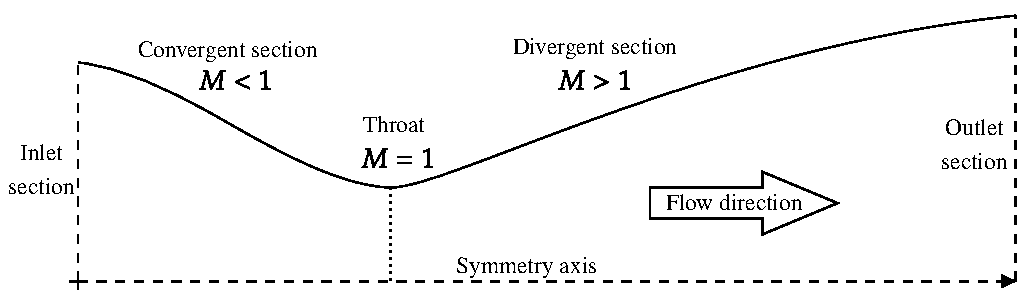
\includegraphics[width=\textwidth]{Figuras/cd_nozzle.pdf} 
    \caption{Schematic representation of a convergent-divergent (De Laval) nozzle. The top panel shows the physical contour, identifying the subsonic converging section, the throat where the flow becomes sonic ($M=1$), and the supersonic diverging section.}
    \label{fig:nozzle_representation}
\end{figure}

The operation of a De Laval nozzle is governed by the principles of isentropic compressible flow theory. As a pressurized gas enters the converging section at subsonic speed, its velocity increases while its pressure and temperature decrease. For a sufficiently low back pressure, the flow accelerates until it reaches sonic velocity (Mach = 1) precisely at the throat, the point of minimum cross-sectional area. This condition is known as choked flow \citep{sutton2010, zucrow1976,white2011}. Beyond the throat, in the diverging section, the flow continues to expand and accelerate into the supersonic regime. A graphical representation of these phenomena is provided in Figure \ref{fig:nozzle_qualitative}. The thrust produced is determined by the momentum of the exiting gas and driven by the pressure differential at the nozzle exit with respect to the inlet section, which shows up the critical importance of maximizing the exhaust velocity for efficient propulsion \citep{anderson2003}.


\begin{figure}[H]
    \centering
    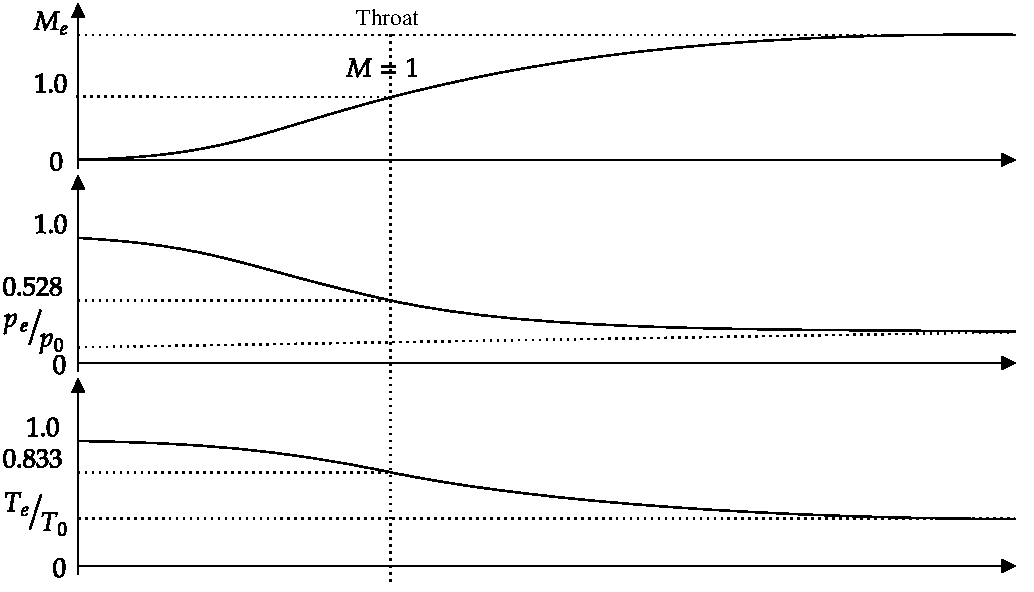
\includegraphics[width=\textwidth]{Figuras/cd_nozzle_qualitative.pdf} 
    \caption{Illustration of the qualitative behavior of key flow properties along the nozzle axis: pressure ($p$) and temperature ($T$) decrease, while Mach number ($M$) increase.}
    \label{fig:nozzle_qualitative}
\end{figure}

\section{Aerothermodynamic Design}

The operational condition within a convergent-divergent nozzle can become exceptionally severe, characterized by extreme temperatures and pressures that result in extreme thermomechanical stresses on the nozzle's wall structure \citep{sutton2010, back1964}. Consequently, a challenge in nozzle design is the management of heat transfer from the hot gas to the nozzle walls. This aerothermodynamic problem is critical to assure the structural integrity and operational reliability of the entire propulsion system . Uncontrolled wall temperatures can lead to material degradation, thermal fatigue, and catastrophic failure \citep{back1964}.

To mitigate these risks, modern high-performance nozzles often incorporate active cooling systems, such as circulating water through channels within the nozzle walls. This makes the design problem into one of conjugate heat transfer (CHT), where the heat transfer within the fluid (convection) is intricately coupled with the heat transfer within the solid structure (conduction), as depicted in Figure \ref{fig:cht_problem}. Accurately predicting the temperature distribution and heat flux at the fluid-solid interface is then not merely an academic exercise but a critical design requirement.

To simplify the complexity of coupled conjugate heat transfer problems, a common approach is to assume steady-state operation. This is a reasonable approximation for many practical applications where transient effects are negligible over the timescale of interest. Under this assumption, the fluid flow can be modeled using the steady-state Reynolds-Averaged Navier–Stokes (RANS) equations, along with appropriate turbulence models to account for the effects of turbulence on heat transfer. The heat transfer in the solid domain is typically modeled by the heat conduction equation, with boundary conditions defined by convective heat transfer from the fluid and any external cooling mechanisms. To further reduce computational cost, the coolant flow is not explicitly modeled. Instead, an average prescribed temperature can be imposed on the cooling surface of the outer nozzle wall, this simplifications are often acceptable for cases with high coolant flow rates \citep{Engblom2007}.

\begin{figure}[H]
    \centering
    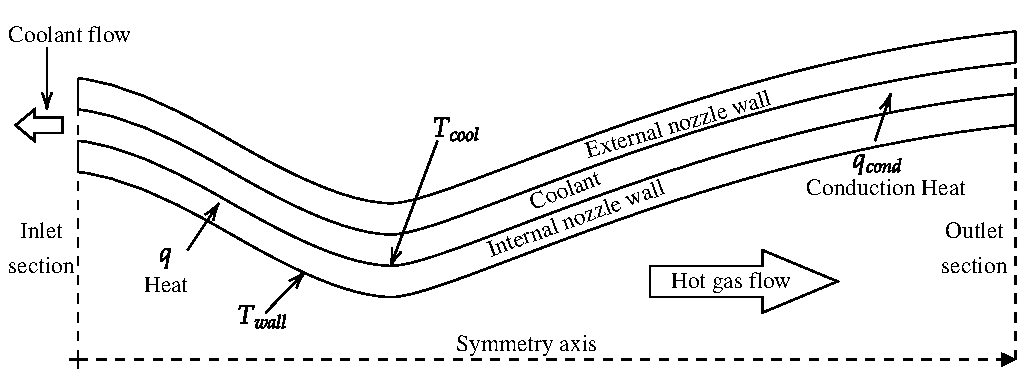
\includegraphics[width=\textwidth]{Figuras/cd_nozzle_cht.pdf}
    \caption{Conceptual diagram of the conjugate heat transfer (CHT) problem in a cooled nozzle wall. The figure shows the coupled physics: convective heat transfer ($q$) from the hot gas flow to the inner wall surface.}
    \label{fig:cht_problem}
\end{figure}

\section{The Computational Bootleneck: Accuracy vs. Cost}

The modeling of such complex CHT phenomena necessitates the use of high-fidelity (HF) computational fluid dynamics (CFD) simulations, which typically solve the Reynolds-Averaged Navier-Stokes (RANS) equations. These simulations are capable of capturing the essential physics of turbulence, viscosity, and heat transfer that govern the system's behavior \citep{wilcox1998}. However, the computational cost associated with these HF simulations can be huge, making them impractical for the mutli-query scenarios often faced in iterative engineering design cycles \citep{hesthaven2016, benner2015, quarteroni2016,hesthaven2016}.

In contrast, low-fidelity (LF) models, such as simplified quasi-one-dimensional (quasi-1D) Euler solvers, are orders of magnitude faster. While these models can capture the essential flow dynamics, like compressibility, their simplification assumptions, prevent them from predicting viscous effects such as boundary layer development and wall heat transfer \citep{moreira2023}. This creates a significant computational dilemma: the models that are fast enough are not accurate enough for the problem at hand, and the models that are accurate enough are far too slow for practical design cycles.

\section{Multifidelity Surrogate Models}

This work addresses the aforementioned computational dilemma by proposing a data-driven, multi-fidelity framework that combines the strengths of both HF and LF models. This approach is centered in the development of a Machine Learning based Reduced Order Model (ML-ROM), a computationally inexpensive surrogate that learns the relationship between the outputs of the HF and LF simulations \citep{moreira2023, hesthaven2016, benner2015}. This surrogate model acts like a sophisticated "black-box" approximator, trained on a pre-computed database of paired LF and HF solutions. The general workflow is depicted in Figure \ref{fig:rom_methodology}. Once trained, the ML-ROM can rapidly generate predictions with dimensinality of the HF model and competitive accuracy, but at a computational cost comparable, or even lower, than the LF model \citep{yu2019, forrester2008, bekemeyer2025}. This paradigm effectively breaks the trade-off between cost and accuracy, enabling the exploration of large design spaces.

\begin{figure}[H]
    \centering
    \begin{minipage}[c]{0.48\textwidth}
        \centering
        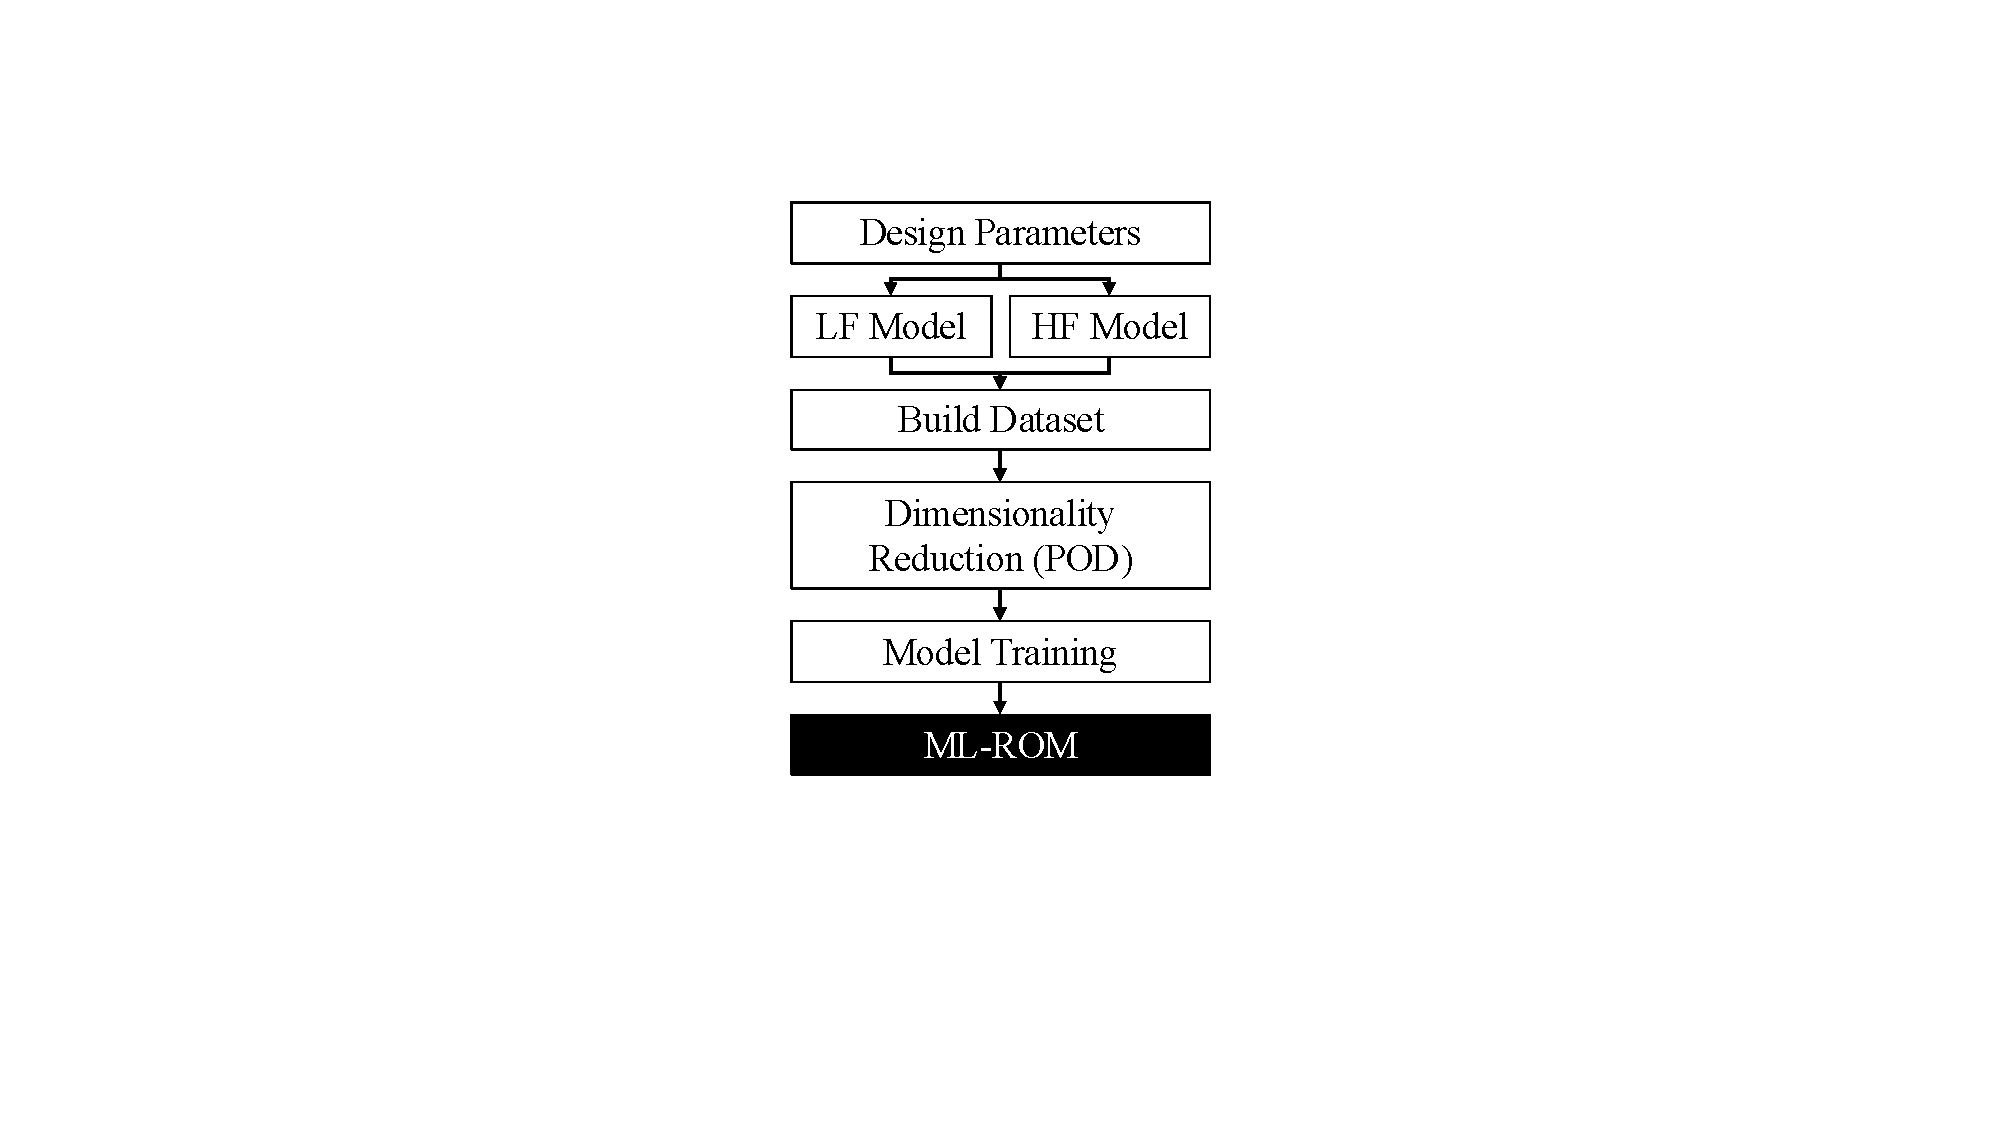
\includegraphics[width=0.5\textwidth]{Figuras/rom_pipeline_a.pdf}
        \subcaption{Offline training stage: generation of paired HF and LF snapshots, POD basis extraction, and surrogate model training.}
        \label{fig:rom_methodology_a}
    \end{minipage}
    \hfill
    \begin{minipage}[c]{0.48\textwidth}
        \centering
        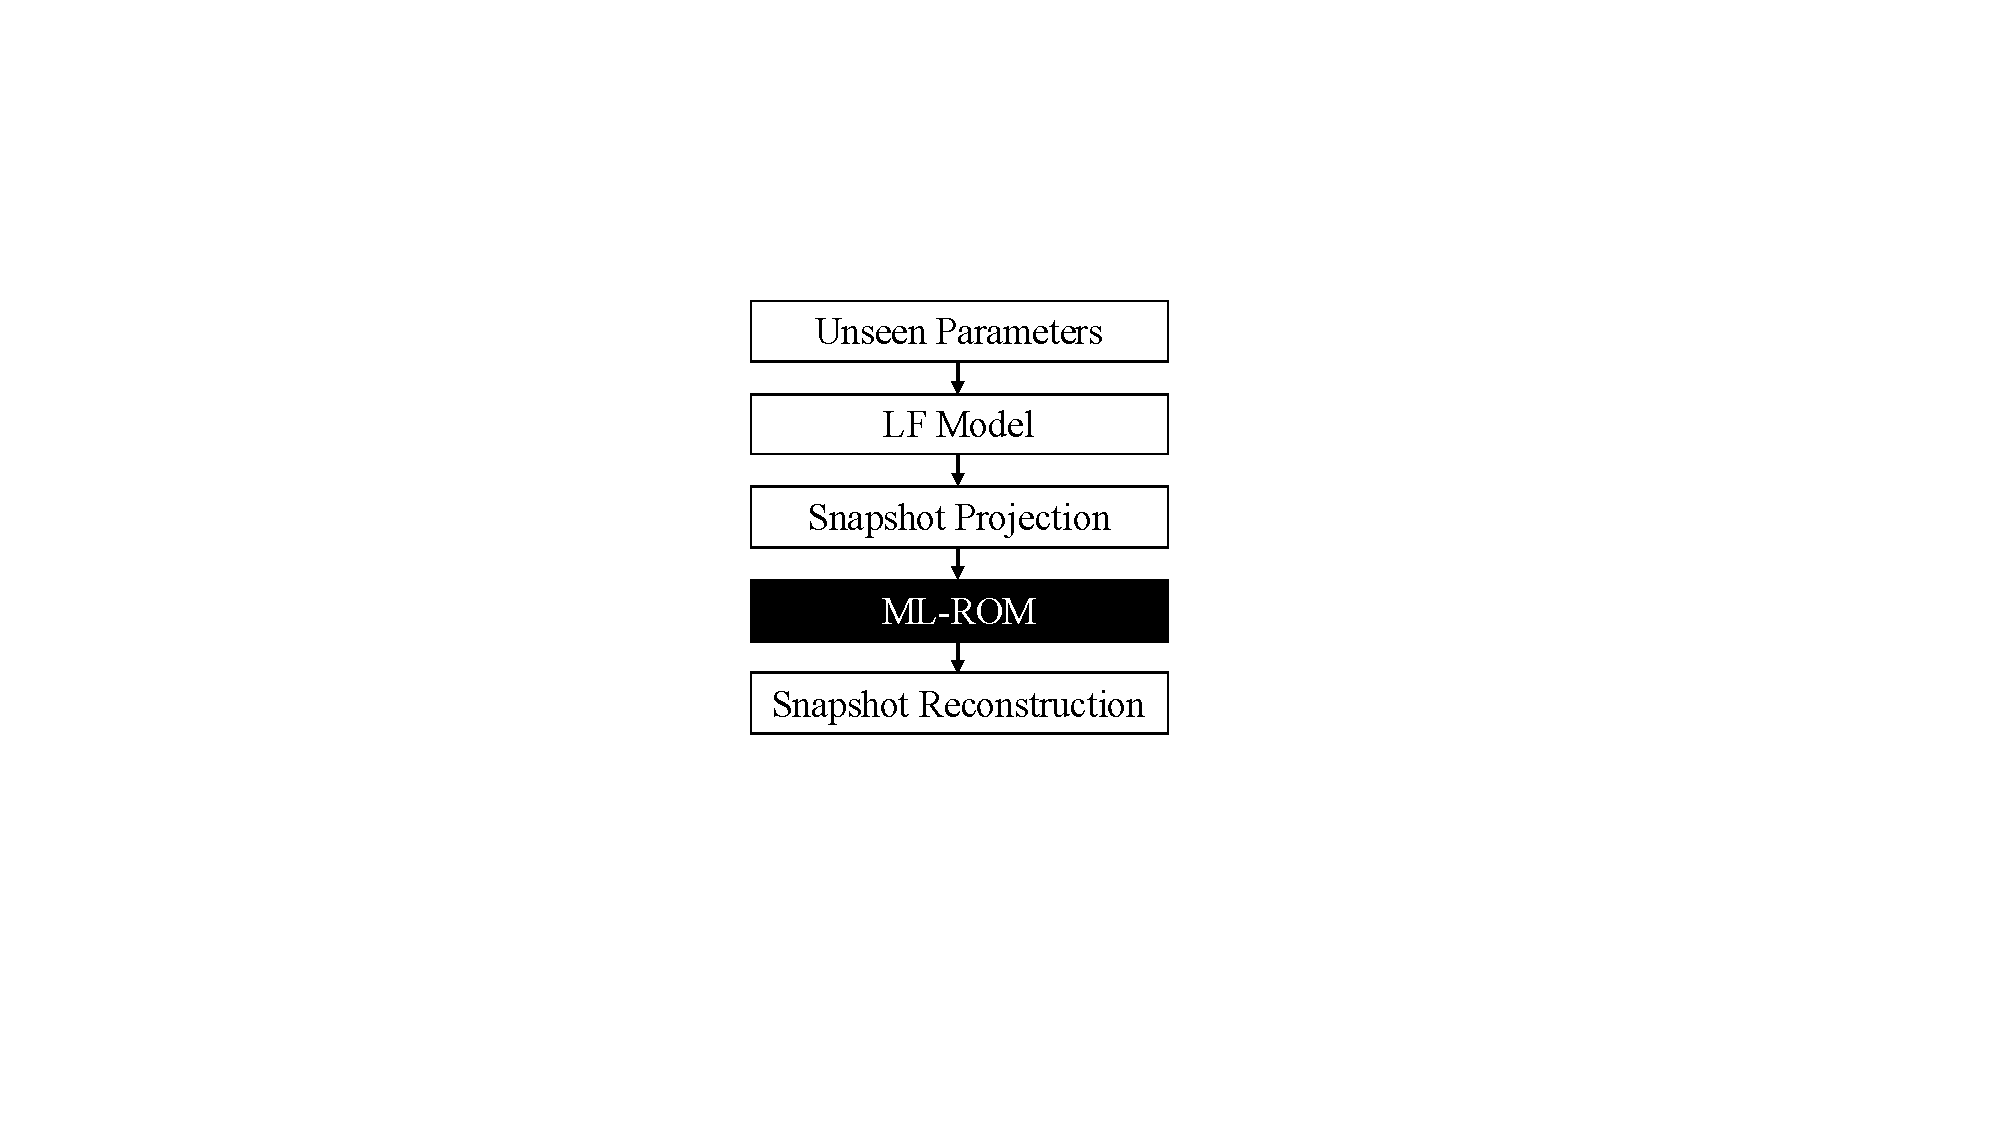
\includegraphics[width=0.5\textwidth]{Figuras/rom_pipeline_b.pdf}
        \subcaption{Online prediction stage: fast LF simulation, projection, surrogate prediction, and HF field reconstruction.}
        \label{fig:rom_methodology_b}
    \end{minipage}
    \caption{The data-driven ML-ROM methodology is divided into two stages. (a) The offline training stage is computationally expensive but performed only once. It involves generating paired high-fidelity (HF) and low-fidelity (LF) simulation snapshots, using Proper Orthogonal Decomposition (POD) to find low-dimensional bases, and training a surrogate model to map the LF coefficients to the HF coefficients. (b) The online prediction stage is computationally cheap and performed during inference on unseen parameters. It involves running a new fast LF simulation, projecting its result onto the LF basis, using the trained surrogate to predict the HF coefficients, and reconstructing the full HF flow field.}
    \label{fig:rom_methodology}
    \end{figure}

\section{Objectives and Contributions}

This work addresses the computational challenge in nozzle aerothermodynamic design by developing a multifidelity data-driven reduced-order model (ROM) able to account for viscous effects and recover 2D flow field solutions from simpler 1D inviscid model solutions. The dissertation was structured around the following key objectives:

\begin{itemize}
    \item \textbf{Implement a multi-fidelity simulation environment:} To develop, verify, and validate both a high-fidelity RANS-CHT model and a computationally inexpensive quasi-1D Euler model to serve as the providers for the data-driven framework.

    \item \textbf{Apply dimensionality reduction to the flow sutions dataset:} To employ Proper Orthogonal Decomposition (POD) to compress the high-dimensional simulation data into a low-dimensional latent space, capturing the most energetic flow features with minimal data loss.

    \item \textbf{Compare surrogate modeling techniques:} To train and evaluate two different machine learning approaches: the Artificial Neural Network (ANN) and the Kriging interpolator, for the task of mapping between the low and high fidelity latent spaces.
    
    \item \textbf{Quantify the framework's performance:} To validate the end-to-end ML-ROM accuracy and computational efficiency on unseen test data.
\end{itemize}

The successful completion of these objectives resulted in the following scientific and technological contributions:

\begin{itemize}
    \item \textbf{A Validated ML-ROM for Nozzle Aerothermodynamics:} The primary contribution is a complete, non-intrusive, data-driven framework capable of accurately reconstructing the 2D flow field and conjugate heat transfer in a cooled nozzle. This provides a practical tool for fast engineering design and optimization.

    \item \textbf{Insight on Surrogate Model Selection:} This work provides a finding for the engineering community: for simple problems with smooth, low-dimensional mappings and limited data, classical statistical methods like Kriging can be competitive and even greater then more complex machine learning architectures in both accuracy and efficiency.

    \item \textbf{Advancement in Computational Efficiency:} By achieving a computational speedup of over 38,000x with minimal loss of accuracy, the framework transforms previously intractable many-query analyses (e.g., design optimization, UQ) into feasible tasks.
\end{itemize}

\section{Dissertation Outline}

The subsequent chapters are structured as follows. Chapter \ref{chap:governing_equations} establishes the theoretical foundations of compressible flow, nozzle aerothermodynamics, and turbulence modeling. Chapter \ref{chap:governing_equations} details the multi-fidelity computational framework, including the setup, verification, and validation of the high and low-fidelity models. Chapter \ref{chap:computational_framework} presents the main data-driven methodology, explaining the principles of Reduced Order Modeling, Proper Orthogonal Decomposition, and the surrogate models employed. Chapter \ref{chap:results_discussion} provides an analysis of the framework's performance, comparing the accuracy and computational efficiency of the different approaches. Finally, Chapter \ref{chap:conclusions_future_work} synthesizes the findings, draws conclusions, and outlines directions for future research.

\chapter{Compressible Flow and Nozzle Aerothermodynamics}
\label{chap:governing_equations}

\section{Governing Equations of Fluid Dynamics}

\subsection{The Euler Equations}

The Euler equations form the mathematical basis for describing inviscid, compressible fluid flow. They represent the conservation of mass, momentum, and energy. For a quasi-one-dimensional flow through a duct with a varying cross-sectional area $S(x)$, these conservation laws can be expressed in the following conservative vector form, as presented in \citep{anderson2003}:
\begin{equation}
    \frac{\partial \mathbf{W}}{\partial t} + \frac{\partial \mathbf{F}}{\partial x} = \mathbf{Q}
    \label{eq:euler_1d}
\end{equation}
,where $\mathbf{W}$ is the vector of conserved variables, $\mathbf{F}$ is the flux vector, and $\mathbf{Q}$ is the source term vector. These vectors are defined as:

\begin{equation}
    \mathbf{W} = 
    \begin{pmatrix}
        \rho S \\
        \rho u S \\
        E_{tot}S
    \end{pmatrix},
    \quad
    \mathbf{F} = 
    \begin{pmatrix}
        \rho u S \\
        (\rho u^2 + p)S \\
        (E_{tot} + p)uS
    \end{pmatrix},
    \quad
    \mathbf{Q} = 
    \begin{pmatrix}
        0 \\
        p \frac{dS}{dx} \\
        0
    \end{pmatrix}
\end{equation}

In these expressions, $\rho$ is the fluid density, $u$ is the axial velocity, $p$ is the static pressure, and $E_{tot}$ is the total energy per unit volume, given by $E_{tot} = \rho(e + u^2/2)$, where $e$ is the specific internal energy. For a calorically perfect gas, the system is closed using the ideal gas law, $p = \rho R T$, and the relation $e = c_v T = p/((\gamma-1)\rho)$, where $\gamma$ is the ratio of specific heats.The source term $\mathbf{Q}$ arises from the dimensional reduction to a single spatial coordinate and accounts for the pressure forces exerted by the nozzle walls on the fluid as the area $S(x)$ changes. 

%The equations are solved numerically using an in-house finite volume solver. This solver employs appropriate flux-splitting schemes (e.g., Steger-Warming and AUSM) to handle the hyperbolic nature of the equations and accurately capture discontinuities like shock waves. To ensure a well-posed problem across different flow regimes, boundary conditions are implemented using the method of characteristics \citep{hirsch1988numerical, hirsch1990numerical}.



\subsection{The Reynolds-Averaged Navier-Stokes (RANS) Equations}
\label{sec:rans_equations}

The physical behavior of a viscous, heat-conducting, and compressible fluid is governed by the Navier-Stokes equations. These equations represent the conservation of mass, momentum, and energy, forming the complete mathematical description for the fluid dynamics simulations conducted in this work. For a comprehensive derivation of these fundamental principles from first principles, the reader is referred to foundational texts on the subject, such as the work by Versteeg and Malalasekera \citep{versteeg2007}.

In a conservative and differential form, as implemented within the SU2 software suite \citep{su2_theory}, the compressible Navier-Stokes equations can be expressed compactly as:

\begin{equation}
    \frac{\partial \mathbf{W}}{\partial t} + \nabla \cdot \mathbf{F}^c(\mathbf{W}) - \nabla \cdot \mathbf{F}^v(\mathbf{W}, \nabla \mathbf{W}) - \mathbf{S} = 0
    \label{eq:rans_compact}
\end{equation}

where $\mathbf{W}$ is the vector of conserved variables, $\mathbf{F}^c$ is the convective flux vector, $\mathbf{F}^v$ is the viscous flux vector, and $\mathbf{S}$ is a source term vector (assumed to be zero for this work). The vectors of conserved variables, convective fluxes, and viscous fluxes are defined, respectively, as:

\begin{equation}
\mathbf{W} = \begin{pmatrix} \rho \\ \rho \mathbf{v} \\ \rho E \end{pmatrix}, \quad
\mathbf{F}^c = \begin{pmatrix} \rho \mathbf{v} \\ \rho \mathbf{v} \otimes \mathbf{v} + p\tens{I} \\ (\rho E + p)\mathbf{v} \end{pmatrix}, \quad
\mathbf{F}^v = \begin{pmatrix} 0 \\ \boldsymbol{\tau} \\ \boldsymbol{\tau} \cdot \mathbf{v} + \mathbf{q} \end{pmatrix}
\end{equation}

In these vectors, $\rho$ is the fluid density, $\mathbf{v}$ is the velocity vector, $E$ is the total energy per unit mass, $p$ is the static pressure, and $\mathbf{I}$ is the identity tensor. The system is closed by the ideal gas law. The viscous stress tensor, $\boldsymbol{\tau}$, for a Newtonian fluid, and the heat flux vector, $\mathbf{q}$, based on Fourier's law of heat conduction, are given by:


\begin{equation}
\boldsymbol{\tau} = \mu \left( \nabla \mathbf{v} + (\nabla \mathbf{v})^T \right) - \frac{2}{3}\mu (\nabla \cdot \mathbf{v})\mathbf{I}
\end{equation}
\begin{equation}
\mathbf{q} = k \nabla T
\end{equation}

where $\mu$ is the dynamic viscosity, $k$ is the thermal conductivity, and $T$ is the temperature.

While the Navier-Stokes equations provide a complete description of fluid motion, their direct numerical simulation (DNS) for the high-Reynolds-number turbulent flows characteristic of aerospace applications is computationally prohibitive. The vast range of turbulent length and time scales would require a grid resolution and time-step size that far exceed current computational capabilities for practical engineering problems. To overcome this limitation, a modeling approach is necessary. This work employs the Reynolds-Averaged Navier-Stokes (RANS) methodology, which involves time-averaging the instantaneous Navier-Stokes equations. This process decomposes flow variables into a mean component and a fluctuating component. The non-linearity of the convective term in the momentum equations gives rise to a new term, the Reynolds stress tensor ($-\rho u_i' u_j'$), which represents the effect of turbulent fluctuations on the mean flow and creates a closure problem.

To close the system of RANS equations, the Reynolds stresses must be modeled. The Boussinesq hypothesis is invoked, which relates the Reynolds stresses to the mean rate of strain in a manner analogous to the relationship between viscous stresses and the strain rate in a Newtonian fluid. This is achieved by introducing a turbulent viscosity, or eddy viscosity ($\mu_t$), which models the momentum transport caused by turbulent eddies. Consequently, the effect of turbulence is accounted for by replacing the molecular dynamic viscosity ($\mu$) with an effective viscosity ($\mu_{\text{eff}} = \mu + \mu_t$). This allows the RANS equations to be solved in a form structurally identical to the original Navier-Stokes equations, with the turbulence model providing the value for $\mu_t$. In this study, the eddy viscosity is calculated using the two-equation Menter's Shear Stress Transport (SST) $k$-$\omega$ model \citep{menter1994}.

%The resulting system of RANS equations was solved for a two-dimensional computational domain using the open-source software suite SU2 \citep{su2_theory}. The spatial discretization of the governing equations was performed using a Finite Volume Method (FVM). Specifically, SU2 employs a median-dual, vertex-based scheme where the control volumes are constructed around the vertices of the primary grid, and fluxes are evaluated at the edges of these control volumes 
%\citep{su2_fvm_scheme}.



\section{Conjugate Heat Transfer and Solid Conduction}
\label{sec:cht_equations}

The comprehensive aerothermodynamic analysis of a cooled structure, such as a rocket nozzle wall, is fundamentally a Conjugate Heat Transfer (CHT) problem. CHT analysis involves the simultaneous solution of heat transfer in distinct but thermally coupled physical domains: the fluid domain, governed by the RANS equations, and the solid domain, governed by the heat conduction equation.

Within the solid domain, the governing equation for heat transfer is the heat conduction equation. As implemented in the SU2 suite \citep{su2_theory}, this equation is expressed in a general, differential form that can account for transient effects

\begin{equation}
\frac{\partial U_s}{\partial t} - \nabla \cdot \mathbf{F}^v(U_s, \nabla U_s) = 0
\label{eq:heat_conduction_transient}
\end{equation}
where the conservative variable $U_s$ and the diffusive flux vector $\mathbf{F}^v$ are defined as:
$$U_s = \rho_s c_{p,s} T_s$$
$$\mathbf{F}^v(U_s, \nabla U_s) = k_s \nabla T_s$$

Here, $T_s$ is the temperature field within the solid, while $\rho_s$, $c_{p,s}$, and $k_s$ are the density, specific heat capacity, and thermal conductivity of the solid material, respectively, which are assumed to be constant. For the steady-state problems considered in this work, the time-derivative term vanishes ($\partial U_s / \partial t = 0$), and the governing equation simplifies to the well-known Laplace equation for heat conduction:

\begin{equation}
\nabla \cdot (k_s \nabla T_s) = 0
\label{eq:heat_conduction_steady}
\end{equation}

This equation is solved numerically within the solid region by SU2's dedicated heat conduction solver. The solver discretizes the equation using a finite volume method (FVM) on a dual grid with vertex-based schemes, where the diffusive flux is evaluated at the midpoint of each control volume edge.

The critical aspect of a CHT simulation is the coupling at the fluid-solid interface. At this boundary, the physical conditions of temperature continuity and heat flux conservation must be enforced. Numerically, this is achieved through an iterative partitioned approach:

\begin{enumerate}
    \item The RANS solver computes the flow field and determines the convective heat flux from the hot gas to the wall.
    \item This heat flux is passed to the solid domain solver and applied as a boundary condition at the interface.
    \item The heat conduction solver solver calculates the resulting temperature distribution throughout the solid wall.
    \item The computed wall temperature at the interface is then passed back to the RANS solver as an updated thermal boundary condition for the fluid domain.
\end{enumerate}

This iterative exchange of boundary data between the fluid and solid solvers continues until the temperature and heat flux values at the interface converge to a stable, self-consistent solution, accurately reflecting the coupled physics of the problem.

\chapter{Computational Framework}
\label{chap:computational_framework}

\section{Low-Fidelity Simulation: The Quasi-1D Euler Solver}
\label{sec:lf_model}

\subsection{Implementation and Numerical Method}

The low-fidelity (LF) model is an in-house solver, developed in C++ leveraging the Eigen library for efficient array computations, and designed for maximum computational efficiency. The solver numerically integrates the quasi-1D Euler equations (Equation~\ref{eq:euler_1d}) on a structured, one-dimensional mesh to predict the core dynamics of the nozzle flow.

A Finite Volume Method is employed for the spatial discretization. To handle the convective terms, the Advection Upstream Splitting Method (AUSM) is used to compute the fluxes at the cell interfaces. This scheme is coupled with a second-order MUSCL (Monotonic Upwind Scheme for Conservation Laws) reconstruction to ensure sharp shock-capturing capabilities without introducing spurious numerical oscillations.

Time integration to a steady-state solution is performed using an explicit, fourth-order Runge-Kutta scheme. The stability of the time marching process is ensured by maintaining a constant Courant-Friedrichs-Lewy (CFL) number of 0.15. Furthermore, characteristic-based boundary conditions are implemented to correctly impose the stagnation properties at the inlet and the prescribed static pressure at the outlet \citep{hirsch1988numerical, hirsch1990numerical}.

\subsection{Numerical Verification}

To verify the implemented LF model, its results were compared against published numerical data from a standard nozzle test case presented by \cite{arina2004}. The geometry of the nozzle is defined by Equation \ref{eq:arinanozzle} within the domain $0 < x < L$, with the throat located at $x_t = 5.0$.

\begin{equation}
S(x)= \begin{cases}
2.5+3\left(\frac{x}{x_t}-1.5\right)\left(\frac{x}{x_t}\right)^2 & , \text { if } x \leqslant x_t \\
3.5-\frac{x}{x_t}\left[6-4.5 \frac{x}{x_t}+\left(\frac{x}{x_t}\right)^2\right] & , \text { if } x>x_t
\end{cases}
\label{eq:arinanozzle}
\end{equation}

The input parameters for the simulation include a stagnation pressure of $P_0 = 104,074 \text{ kPa}$ and a stagnation temperature of $T_0 = 291.3 \text{ K}$ at the inlet. At the outlet, a static pressure of $P_{\text{exit}} = 83,049 \text{ kPa}$ is prescribed. Air is modeled as an ideal gas with a specific gas constant $R = 287 \text{ J/kg}\cdot\text{K}$ and a ratio of specific heats $\gamma = 1.4$.

The comparison, shown in Figure~\ref{fig:lf_verification}, reveals excellent agreement between the in-house solver's predictions and the reference data. Both the pressure and density profiles along the nozzle are accurately reproduced, including the precise capture of the shock wave's position and strength. This verification confirms the LF model provides a reliable and accurate representation of the core, one-dimensional flow dynamics. The entire simulation for this verification case converges in under 2 seconds on a standard desktop CPU, validating its role as a computationally inexpensive model for the multi-fidelity framework.

\begin{figure}[H]
    \centering
    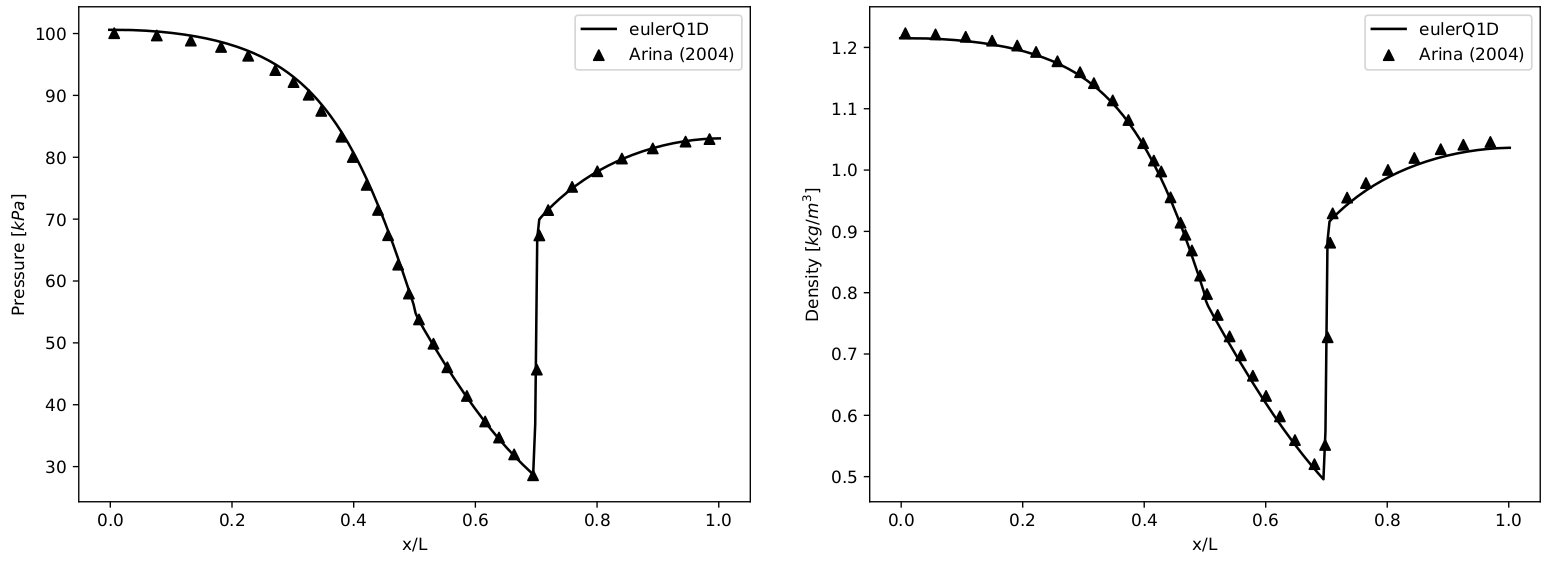
\includegraphics[width=\textwidth]{Figuras/arina_validation.png}
    \caption{Verification of the low-fidelity (LF) quasi-1D Euler solver. Comparison of the in-house solver's predictions against reference numerical data from \citep{arina2004} for a standard nozzle test case with a shock wave. (a) Pressure profile. (b) Density profile. The excellent agreement, including the shock position and strength, verifies the correctness of the LF model implementation.}
    \label{fig:lf_verification}
\end{figure}

% \section{Low-Fidelity Simulation: The Quasi-1D Euler Approach}

% The low-fidelity model is an in-house, quasi-one-dimensional Euler solver designed for maximum computational efficiency \citep{moreira2023}. It solves the conservation laws for an inviscid, ideal gas on a regular 1D mesh. The numerical scheme employs the finite volume method with Steger-Warming for spatial discretization and the AUSM method for flux evaluation. A fourth-order Runge-Kutta integrator is used for time marching to a steady-state solution \citep{moreira2023}.


% \subsection{Numerical Verification}

% To verify this simplified model, its results were compared against published numerical data from a standard nozzle test case presented by Arina (2004). The geometry of the nozzle is defined by Equation~\ref{eq:arinanozzle} within the domain $0 < x < L$, with the throat located at $x_t = 5.0$.

% \begin{equation}
% S(x)= \begin{cases}
% 2.5+3\left(\frac{x}{x_t}-1.5\right)\left(\frac{x}{x_t}\right)^2 & , \text { if } x \leqslant x_t \\
% 3.5-\frac{x}{x_t}\left[6-4.5 \frac{x}{x_t}+\left(\frac{x}{x_t}\right)^2\right] & , \text { if } x>x_t
% \end{cases}
% \label{eq:arinanozzle}
% \end{equation}

% The input parameters for the simulation include a stagnation pressure of $P_0 = 104,074 \text{ kPa}$ and a stagnation temperature of $T_0 = 291.3 \text{ K}$ at the inlet. At the outlet, a static pressure of $P_{exit} = 83,049 \text{ kPa}$ is prescribed. Air is modeled as an ideal gas with a specific gas constant $R = 287 \text{ J/kg}\cdot\text{K}$ and a ratio of specific heats $\gamma = 1.4$.

% The comparison, shown in Figure \ref{fig:lf_verification}, reveals excellent agreement between the in-house solver's predictions and the reference data from \cite{ARINA2004409}. Both the pressure and density profiles along the nozzle are accurately reproduced, including the precise capture of the shock wave's position and strength. This verification confirms that despite its inherent simplifications, the low-fidelity model provides a reliable and accurate representation of the core, one-dimensional flow dynamics \citep{moreira2023}.

% \begin{figure}[H]
%     \centering
%     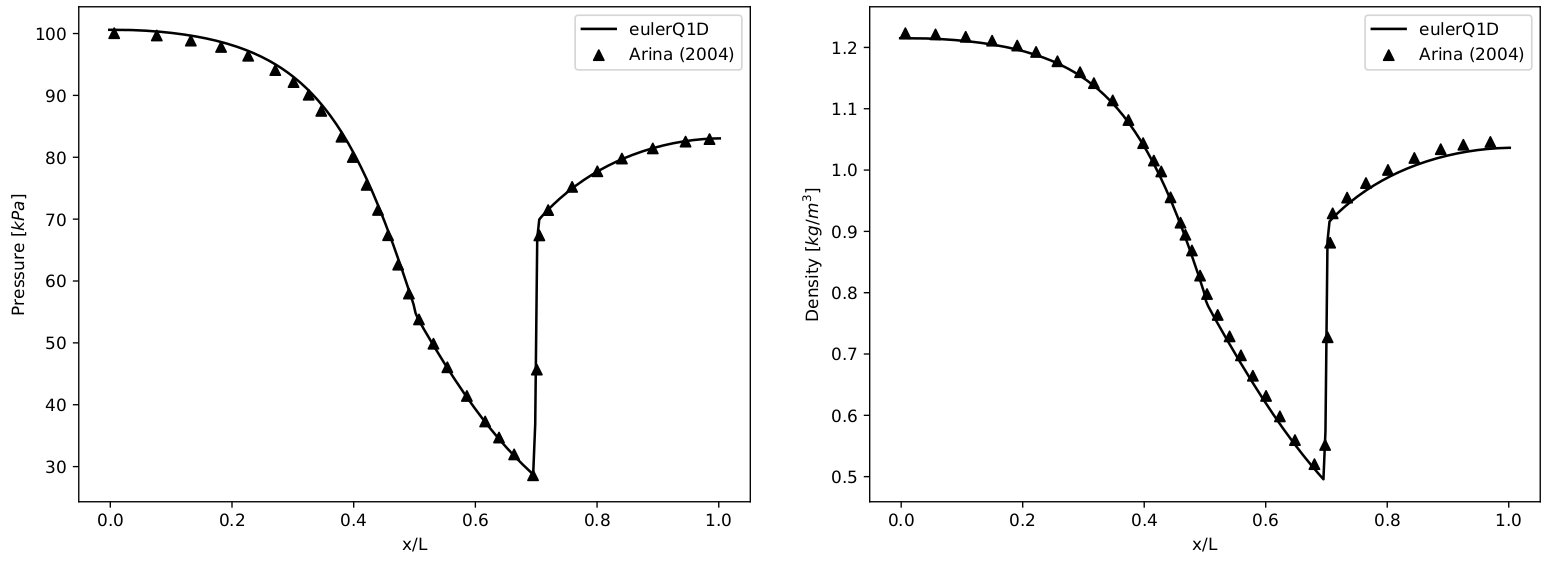
\includegraphics[width=\textwidth]{Figuras/arina_validation.png}
%     \caption{Verification of the low-fidelity (LF) quasi-1D Euler solver. Comparison of the in-house solver's predictions against reference numerical data from Arina (2004) for a standard nozzle test case with a shock wave. (a) Pressure profile. (b) Density profile. The excellent agreement, including the shock position and strength, verifies the correctness of the LF model implementation.}
%     \label{fig:lf_verification}
% \end{figure}

\section{High-Fidelity Simulation: The 2D RANS-CHT Approach}

\subsection{The SU2 CFD Suite}

The high-fidelity simulations were conducted using the SU2 software suite, an open-source platform developed for multiphysics analysis and design optimization. SU2 (Stanford University Unstructured) is a collection of C++ and Python-based tools designed to solve partial differential equations on unstructured meshes using state-of-the-art numerical methods \citep{economon2016}. Its robust capabilities for handling compressible flows, conjugate heat transfer, and a wide range of turbulence models make it a suitable choice for this research \citep{economon2016, palacios2022}.

\subsection{Model Setup}

The high-fidelity model was configured to solve the conjugate heat transfer problem in its entirety. Within the fluid domain, the Reynolds-Averaged Navier-Stokes (RANS) equations were solved using a finite volume method. The Menter's SST turbulence model was employed to close the equations, as detailed in section \ref{sec:rans_equations}. In the solid domain, representing the nozzle wall, the energy equation was solved to model heat conduction. To achieve a steady-state solution, the simulation utilized an implicit Euler integration method coupled with time marching until convergence was reached at the fluid-solid interface.

The boundary conditions were specified to represent the nozzle's physical operation. At the fluid inlet, total pressure ($p_{0in}$) and total temperature ($T_{0in}$) were defined as stagnation properties. The outlet was defined with a static pressure condition ($p_{\text{exit}}$). The nozzle's centerline was treated as a symmetry axis. A no-slip condition was applied at the inner nozzle wall, which also served as the coupled interface for the conjugate heat transfer (CHT) problem. On the outer surface of the solid wall, representing the cooling channel, a constant temperature of 300 K was imposed, a common simplification for high-efficiency cooling systems %\citep{engblom2007}.


\subsection{Numerical Verification: Grid Independence Study}

A critical step in any CFD analysis is verification, which ensures that the numerical solution is not an artifact of the computational grid. A grid independence study was performed using the Grid Convergence Index (GCI) method proposed by Roache (1994) to quantify the discretization error \citep{moreira2023}. Three structured grids of increasing refinement were generated, as detailed in Table \ref{tab:grid_independence_domains}.

\begin{table}[H]
\centering
\caption{Numerical domains for the grid independence study. The table details the number of nodes in the axial ($N_x$) and radial ($N_y$) directions, the total number of cells ($N_{cells}$), the grid refinement ratio ($r$), and the approximate near-wall grid spacing in wall units ($Y^{+}$) \citep{moreira2023}.}
\label{tab:grid_independence_domains}
\begin{tabular}{lccccc}
\toprule
 & $N_x$ & $N_y$ & $N_{cells}$ & $r$ & $Y^{+}$ \\
\midrule
\textbf{Grid 1} & 270 & 440 & 118091 & 1.3 & $\approx1$ \\
\textbf{Grid 2} & 210 & 330 & 68761 & 1.3 & $\approx2$ \\
\textbf{Grid 3} & 160 & 250 & 39591 & & $\approx3$ \\
\bottomrule
\end{tabular}
\end{table}

Figure \ref{fig:grid_choosen} illustrates the computational domains selected by the GCI analysis. The grids were designed to ensure that the near-wall region was adequately resolved, with the wall spacing ($Y^{+}$) kept below 3, which is generally acceptable for RANS simulations \citep{moreira2023}.

\begin{figure}[H]
    \centering
    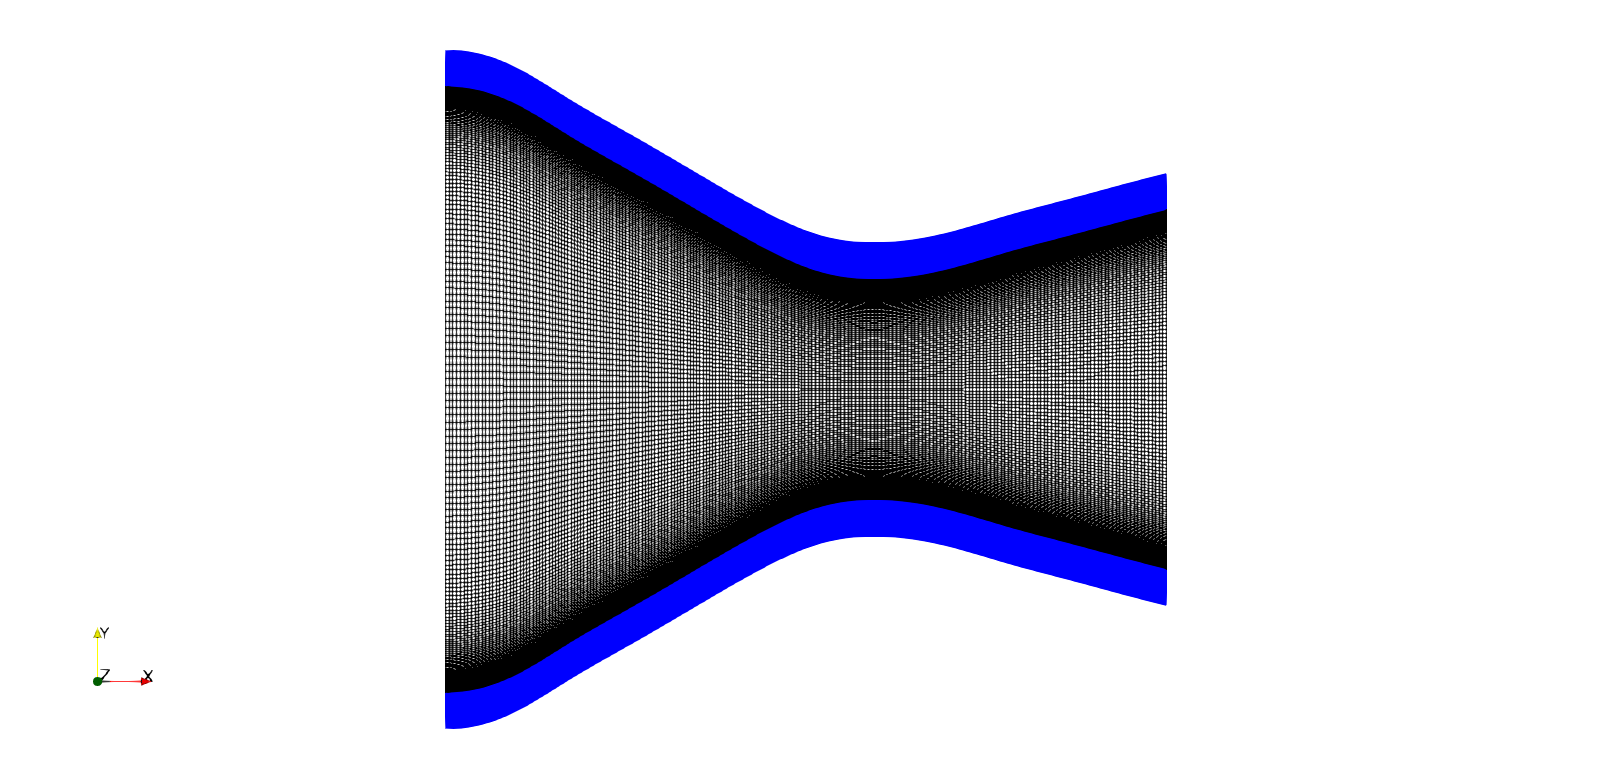
\includegraphics[width=\textwidth]{Figuras/grid_choosen.png}
    \caption{Computational domains used in the grid independence study. The figure shows the three grids with increasing refinement, highlighting the near-wall region resolution.}
    \label{fig:grid_choosen}
\end{figure}

The GCI was calculated for key output quantities: average heat flux along the wall ($q$), pressure along the centerline ($p$), and temperature at the wall ($T$). The results, summarized in Table \ref{tab:grid_independence_results}, show that the solutions exhibit monotonic and asymptotic convergence, as indicated by the positive order of convergence ($p_{GCI}$) and small GCI values. An asymptotic ratio ($GCI_{asymptotic}$) close to 1 signifies that the solution is in the asymptotic range of convergence and is effectively grid-independent. Based on this rigorous analysis, Grid 2 was selected for all subsequent high-fidelity simulations, as it provided a reliable solution with a manageable cell count. This verification process is fundamental to the entire study, as it establishes a credible and converged high-fidelity baseline against which the reduced-order models are ultimately judged.

\begin{table}[H]
\centering
\caption{Results for the grid independence study for average heat flux ($q$), pressure ($p$), and wall temperature ($T$). The analysis confirms asymptotic convergence, justifying the selection of Grid 2 \citep{moreira2023}.}
\label{tab:grid_independence_results}
\begin{tabular}{lcccccc}
\toprule
 & $q$ $[W/m^2]$ & $N_{cells}$ & $r$ & GCI & $GCI_{asymptotic}$ & $p_{GCI}$ \\
\midrule
\textbf{Grid 1} & $519 \times 10^3$ & 118091 & 1.3 & 6.95\% & & \\
\textbf{Grid 2} & $502 \times 10^3$ & 68761 & 1.3 & 11.40\% & 1.034 & 1.71 \\
\textbf{Grid 3} & $475 \times 10^3$ & 39591 & & & & \\
\midrule
 & $p$ [kPa] & $N_{cells}$ & $r$ & GCI & $GCI_{asymptotic}$ & $p_{GCI}$ \\
\midrule
\textbf{Grid 1} & $737 \times 10^3$ & 118091 & 1.3 & 0.23\% & & \\
\textbf{Grid 2} & $736 \times 10^3$ & 68761 & 1.3 & 0.30\% & 1.001 & 1.02 \\
\textbf{Grid 3} & $736 \times 10^3$ & 39591 & & & & \\
\midrule
 & $T$ [K] & $N_{cells}$ & $r$ & GCI & $GCI_{asymptotic}$ & $p_{GCI}$ \\
\midrule
\textbf{Grid 1} & 518 & 118091 & 1.3 & 0.17\% & & \\
\textbf{Grid 2} & 520 & 68761 & 1.3 & 0.47\% & 0.998 & 3.73 \\
\textbf{Grid 3} & 523 & 39591 & & & & \\
\bottomrule
\end{tabular}% 
\end{table}


\subsection{Numerical Validation with Experimental Data}

Following verification, the high-fidelity model was validated by comparing its predictions against experimental data for test case no. 313 from \citep{back1964}. This validation process faced certain challenges due to incomplete information in the reference study, such as the exact composition of the nozzle wall, which was assumed to be AISI 302 stainless steel. Furthermore, the boundary condition for the outer cooling wall was simplified to a constant temperature of 300 K. Despite these limitations, the validation showed promising results, as seen in Figure \ref{fig:hf_validation}. The predicted pressure distribution along the nozzle centerline demonstrated good agreement with the experimental measurements. While the predicted wall temperature showed a slight deviation, likely attributable to the simplified boundary conditions and material property assumptions, the overall agreement was sufficient to establish confidence in the high-fidelity model's ability to capture the essential physics of the problem.


\begin{figure}[H]
    \centering
    \begin{minipage}[c]{0.9\textwidth}
        \centering
        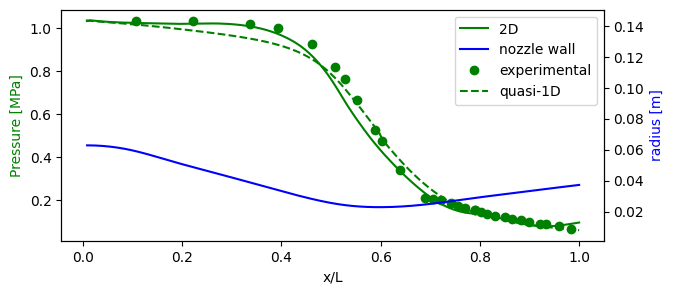
\includegraphics[width=\textwidth]{Figuras/hf_validation_pressure.png}
        \subcaption{Validation of centerline pressure distribution: comparison between SU2 simulation and experimental data.}
        \label{fig:hf_validation_pressure}
    \end{minipage}
    \vspace{1em}
    \begin{minipage}[c]{0.9\textwidth}
        \centering
        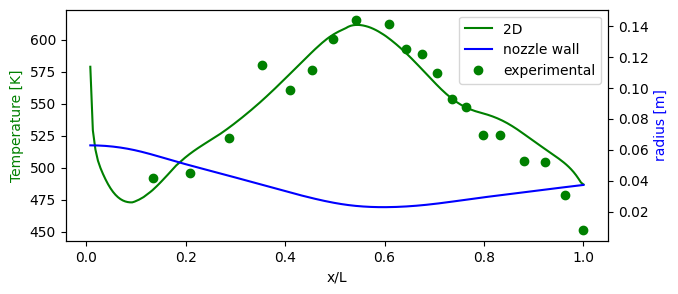
\includegraphics[width=\textwidth]{Figuras/hf_validation_temperature.png}
        \subcaption{Validation of wall temperature distribution: comparison between SU2 simulation and experimental data.}
        \label{fig:hf_validation_temperature}
    \end{minipage}
    \caption{Comparison of high-fidelity SU2 simulation results with experimental data from \citep{back1964} for test case no. 313. (a) Centerline pressure distribution. (b) Wall temperature distribution.}
    \label{fig:hf_validation}
\end{figure}


\section{Parametric Data Generation for Model Training}

To train the data-driven surrogate models, a comprehensive dataset mapping the low-fidelity inputs to the high-fidelity outputs was required. This dataset was generated by running 181 paired simulations, where each pair consisted of one LF and one HF simulation for the same set of boundary conditions. The key parameter varied across these simulations was the inlet total temperature ($T_{0in}$), which was sampled across a range of 285 K to 1115 K.

While the inlet total temperature was varied, other key boundary conditions were held constant across all 181 simulations to isolate its effect. Specifically, the inlet total pressure ($P_{0in}$) was fixed at 1191.0 kPa and the outlet static pressure ($P_{\text{exit}}$) was set to 101.0 kPa.

Each simulation result constitutes a "snapshot" of the flow field. Specifically, a high-fidelity (HF) snapshot is a single vector containing the complete 2D field data, while a low-fidelity (LF) snapshot consists of the flattened 1D data from the Euler solver. The collection of these paired snapshots forms the final dataset used for the subsequent dimensionality reduction and model training stages.

For each simulation $j$, the high-fidelity snapshot vector $\mathbf{x}_{h,j} \in \mathbb{R}^{m_h}$ is constructed by concatenating the flattened vectors of pressure ($\mathbf{p}_h$), temperature ($\mathbf{T}_h$), and Mach number ($\mathbf{M}_h$) from all $N_{nodes}$ grid points, along with the wall heat flux ($\mathbf{q}_w$) at the $N_{wall}$ wall points:
\begin{equation}
    \mathbf{x}_{h,j} = 
    \begin{bmatrix}
        \mathbf{p}_h \\
        \mathbf{T}_h \\
        \mathbf{M}_h \\
        \mathbf{q}_w
    \end{bmatrix}_j
    , \quad \text{where } m_h = 3 \times N_{nodes} + N_{wall}.
\end{equation}
Similarly, the corresponding low-fidelity snapshot vector $\mathbf{x}_{l,j} \in \mathbb{R}^{m_l}$ is composed of the flattened 1D data for pressure ($\mathbf{p}_l$), temperature ($\mathbf{T}_l$), and Mach number ($\mathbf{M}_l$) from the $N_{1D}$ points of the Euler solver's mesh:
\begin{equation}
    \mathbf{x}_{l,j} = 
    \begin{bmatrix}
        \mathbf{p}_l \\
        \mathbf{T}_l \\
        \mathbf{M}_l
    \end{bmatrix}_j
    , \quad \text{where } m_l = 3 \times N_{1D}.
\end{equation}


To ensure efficient and uniform exploration of this parameter space, Latin Hypercube Sampling (LHS) was employed. LHS is a statistical method for Design of Experiments (DoE) that generates a more representative sample of the parameter space compared to simple random sampling, making it a standard and effective practice for generating training data for surrogate models \citep{yu2019}. The resulting dataset of 181 snapshot pairs was then partitioned into three subsets for the machine learning workflow: 145 pairs for training the models, 18 for validation during the training process to prevent overfitting, and a final 18 pairs held out as a blind test set to evaluate the final performance of the trained models. A summary of the dataset is provided in Table \ref{tab:dataset_summary}.

\begin{table}[H]
\centering
\caption{Summary of the dataset generation and partitioning for machine learning model development.}
\label{tab:dataset_summary}
\begin{tabular}{lcccc}
\toprule
\textbf{Purpose} & \textbf{\# of Samples} & \textbf{Sampling Method} & \textbf{Parameter Varied} & \textbf{Range} \\
\midrule
Training & 145 & LHS &  $T_{0in}$ & 285 K - 1115 K \\
Validation & 18 & LHS & $T_{0in}$ & 285 K - 1115 K \\
Testing & 18 & LHS &  $T_{0in}$ & 285 K - 1115 K \\
\midrule
\textbf{Total} & \textbf{181} & & & \\
\bottomrule
\end{tabular}
\end{table}


\chapter{Data-Driven Flow Reconstruction via Reduced Order Modeling}
\label{chap:rom_framework}

\section{Reduced Order Modeling (ROM)}

Reduced Order Modeling is a paradigm designed to address the computational bottleneck inherent in high-fidelity simulations. ROMs create computationally inexpensive, low-dimensional surrogate models that approximate the behavior of a full-order, complex system \citep{brunton2019, stabile2021}. These models are particularly valuable in many-query contexts like optimization, control, and uncertainty quantification, where repeated evaluations of the full model are infeasible. ROMs can be broadly categorized into two classes: intrusive and non-intrusive. Intrusive methods, such as Galerkin projection, require modification of the governing equation solvers. In contrast, non-intrusive methods are purely data-driven, treating the full-order model as a black box and learning the input-output relationship from simulation data \citep{hesthaven2016, benner2015}. The framework developed in this dissertation falls into the non-intrusive category.

\section{Proper Orthogonal Decomposition (POD)}

A foundational step in building an effective ROM is dimensionality reduction. Proper Orthogonal Decomposition (POD) is a powerful mathematical technique for extracting a low-dimensional basis that optimally captures the variance within a high-dimensional dataset \citep{berkooz1993, sirovich1987, holmes2012}. Mathematically, POD is equivalent to Principal Component Analysis (PCA) and is implemented via the Singular Value Decomposition (SVD) of the data matrix. The method decomposes a complex, spatiotemporal field into a set of orthogonal spatial modes (the POD modes) and corresponding temporal coefficients. These modes are hierarchical; the first mode captures the most energy (or variance) in the data, the second captures the most of the remaining energy, and so on. This property allows for an extremely efficient, low-rank approximation of the original data by retaining only the first few most energetic modes \citep{rowley2017, taira2017}. The core of the method is the SVD of a snapshot matrix $\mathbf{X}$, which is detailed in the following section. A full mathematical formulation of POD is provided in Appendix B.

\subsection{The Snapshot Method}

The specific implementation of POD used in this study is the snapshot method. The process begins by assembling the individual snapshot vectors, which were defined in the previous chapter, into high-fidelity and low-fidelity snapshot matrices. Each of the $n=181$ snapshot vectors from the simulations becomes a column in its respective matrix, $\mathbf{X}_h \in \mathbb{R}^{m_h \times n}$ and $\mathbf{X}_l \in \mathbb{R}^{m_l \times n}$. This column-wise assembly is represented as:
\begin{equation}
    \mathbf{X}_h = 
    \begin{bmatrix}
        | & | & & | \\
        \mathbf{x}_{h,1} & \mathbf{x}_{h,2} & \dots & \mathbf{x}_{h,n} \\
        | & | & & |
    \end{bmatrix}
    , \quad
    \mathbf{X}_l = 
    \begin{bmatrix}
        | & | & & | \\
        \mathbf{x}_{l,1} & \mathbf{x}_{l,2} & \dots & \mathbf{x}_{l,n} \\
        | & | & & |
    \end{bmatrix}
    \label{eq:snapshot_matrix}
\end{equation}
where $m_h$ and $m_l$ are the total number of degrees of freedom for a single high- and low-fidelity snapshot, respectively. These matrices contain the complete dataset and serve as the direct input for the Singular Value Decomposition (SVD).

The SVD is then performed on these matrices. For a generic snapshot matrix $\mathbf{X}$, the SVD is given by:
\begin{equation}
\mathbf{X} = \mathbf{U} \mathbf{\Sigma} \mathbf{V}^T
\end{equation}
where $\mathbf{U} \in \mathbb{R}^{m \times m}$ is an orthogonal matrix whose columns are the left singular vectors (the POD spatial modes), $\mathbf{\Sigma} \in \mathbb{R}^{m \times n}$ is a diagonal matrix of singular values $\sigma_i$, and $\mathbf{V} \in \mathbb{R}^{n \times n}$ is an orthogonal matrix whose columns are the right singular vectors (related to the temporal coefficients).

By projecting the high-dimensional snapshot data onto a small number of these modes (a truncated basis $\mathbf{\Psi}_r = [\mathbf{u}_1, \dots, \mathbf{u}_r]$), one obtains a set of low-dimensional coefficients that serve as a compact representation of the full system state. The approximation of a snapshot $\mathbf{x}_j$ and the calculation of its coefficient vector $\mathbf{a}_j$ are given by:
\begin{equation}
\mathbf{x}_j \approx \mathbf{\Psi}_r \mathbf{a}_j
\end{equation}
\begin{equation}
\mathbf{a}_j = \mathbf{\Psi}_r^T \mathbf{x}_j
\end{equation}

\subsection{Application and Efficacy}

The application of POD to the nozzle flow dataset yielded a remarkable degree of dimensionality reduction. The high-fidelity state, originally described by 208,110 degrees of freedom (the number of grid points times the number of variables), was accurately represented using only 3 POD modes. The effectiveness of this compression is visualized in Figure \ref{fig:pod_results}. The energy spectrum shows a rapid decay, indicating that the vast majority of the system's variance is captured by the first few modes. The projection error associated with this truncation was exceptionally low, with an average global relative error in the temperature field of just 0.0006\% and a maximum error for a sample case of only 0.0133\% \citep{moreira2023}. This demonstrates the extraordinary efficiency of POD in compressing the vast amount of information contained in the CFD solutions into a highly compact, latent variable representation with negligible loss of information.

\begin{figure}[H]
    \centering
    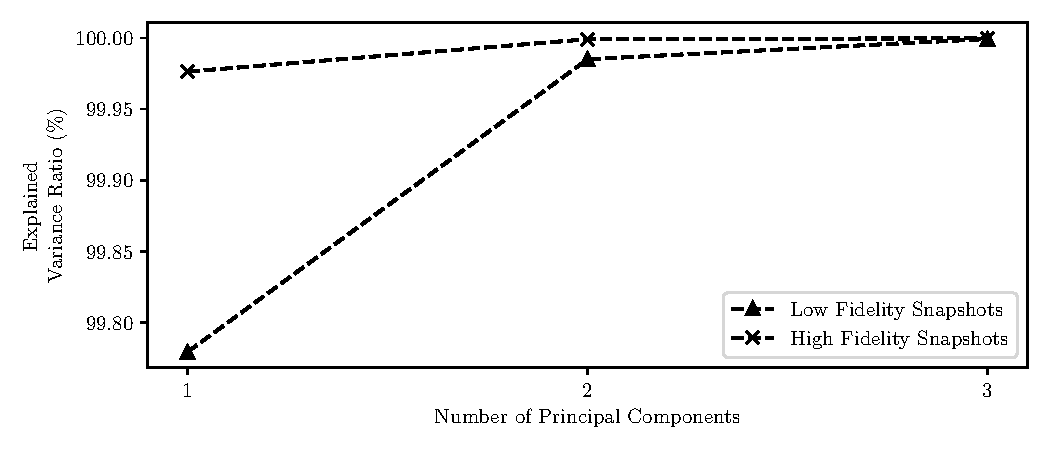
\includegraphics[width=\textwidth]{../latex_src/Figuras/POD_energy.pdf}
    \caption{Efficacy of Proper Orthogonal Decomposition (POD). (a) Normalized energy spectrum, showing the rapid decay of singular values, which indicates that the first few modes capture most of the system's energy. (b) Visualization of the first three dominant spatial POD modes for the temperature field, representing the fundamental patterns of temperature variation across the dataset.}
    \label{fig:pod_results}
\end{figure}

This powerful compression is the key enabler for the entire surrogate modeling framework. The original problem—mapping a 633-dimensional low-fidelity state vector to a 208,110-dimensional high-fidelity state vector—is a high-dimensional regression task that would be intractable for any machine learning model without an enormous dataset. POD transforms this problem. It acts as an expert feature extractor, identifying the fundamental building blocks (the modes) of the flow. The complex task of learning the spatially distributed physics is thus converted into a much simpler one: learning the mapping between the 10 coefficients of the low-fidelity model and the 10 coefficients of the high-fidelity model. In this synergistic partnership, POD performs the heavy lifting of identifying the relevant physical structures, while the surrogate model learns the relatively simple correlation between their amplitudes. This synergy is the cornerstone of the framework's success.

\section{Surrogate Modeling for Latent Space Mapping}

Once the dimensionality of the problem has been reduced via POD, a surrogate model is required to learn the nonlinear mapping from the low-fidelity latent space to the high-fidelity latent space. This study compares two distinct approaches for this task: an Artificial Neural Network and a Kriging interpolator.

The goal is to construct a function, $f_{\text{surrogate}}$, that approximates the relationship between the low-fidelity (LF) and high-fidelity (HF) POD coefficients. Given a training dataset of $N_{\text{train}}$ paired coefficients, $\{ (\mathbf{a}_{l,j}, \mathbf{a}_{h,j}) \}_{j=1}^{N_{\text{train}}}$, the surrogate model aims to learn the mapping:

\begin{equation}
    \mathbf{a}_h \approx \hat{\mathbf{a}}_h = f_{\text{surrogate}}(\mathbf{a}_l)
    \label{eq:surrogate_mapping}
\end{equation}

where $\mathbf{a}_l \in \mathbb{R}^{d_l}$ is the vector of LF coefficients, $\mathbf{a}_h \in \mathbb{R}^{d_h}$ is the vector of true HF coefficients, and $\hat{\mathbf{a}}_h$ is the prediction from the surrogate model. This study compares two distinct approaches for this task: an Artificial Neural Network and a Kriging interpolator.


\subsection{The Artificial Neural Network (ANN) Approximator}

Artificial Neural Networks are powerful computational models inspired by biological neural systems, renowned for their ability to act as universal function approximators \citep{hornik1989}. The specific architecture used here is a dense Multilayer Perceptron (MLP), which consists of an input layer, multiple hidden layers of interconnected "neurons," and an output layer. Each connection has an associated weight, and each neuron applies a nonlinear activation function to its input. The output $o_j$ of a single neuron is calculated as:

\begin{equation}
o_j = f \left( \sum_{i} w_{ij} x_i + b_j \right)
\end{equation}

where $w_{ij}$ are the weights, $x_i$ are the inputs from the previous layer, $b_j$ is a bias term, and $f$ is a nonlinear activation function. The network "learns" by adjusting these weights and biases through a process called back-propagation, which uses gradient descent to minimize a loss function (e.g., Mean Squared Error) between the network's predictions and the true data \citep{yu2019}.

The entire MLP represents a complex, nested function, $f_{\text{ANN}}$, parameterized by the set of all weights $\mathbf{W}$ and biases $\mathbf{b}$. For a given input vector of LF coefficients $\mathbf{a}_l$, the network produces a prediction for the HF coefficients $\hat{\mathbf{a}}_h$:

\begin{equation}
    \hat{\mathbf{a}}_h = f_{\text{ANN}}(\mathbf{a}_l; \mathbf{W}, \mathbf{b})
\end{equation}

The network "learns" by adjusting the parameters $\mathbf{W}$ and $\mathbf{b}$ through a process called back-propagation, which uses gradient descent to minimize a loss function. In this work, the Mean Squared Error (MSE) between the network's predictions and the true data is minimized:

\begin{equation}
    \mathcal{L}(\mathbf{W}, \mathbf{b}) = \frac{1}{N_{\text{train}}} \sum_{j=1}^{N_{\text{train}}} \| \mathbf{a}_{h,j} - f_{\text{ANN}}(\mathbf{a}_{l,j}; \mathbf{W}, \mathbf{b}) \|_2^2
\end{equation}

The implementation in this work utilized the TensorFlow library to construct a dense MLP with the architecture illustrated in Figure~\ref{fig:ann_architecture}: an input layer with 3 neurons (for the 3 LF POD coefficients), 10 hidden layers each containing 10 neurons, and an output layer with 3 neurons (for the 3 HF POD coefficients). The hyperbolic tangent ('tanh') was used as the activation function for the hidden layers, and the ADAM optimizer was employed for efficient training. The training history, shown in Figure~\ref{fig:ann_loss}, displays a rapid decrease in both the training and validation loss functions, indicating effective learning of the mapping between the latent spaces without significant overfitting.

\begin{figure}[H]
    \centering
    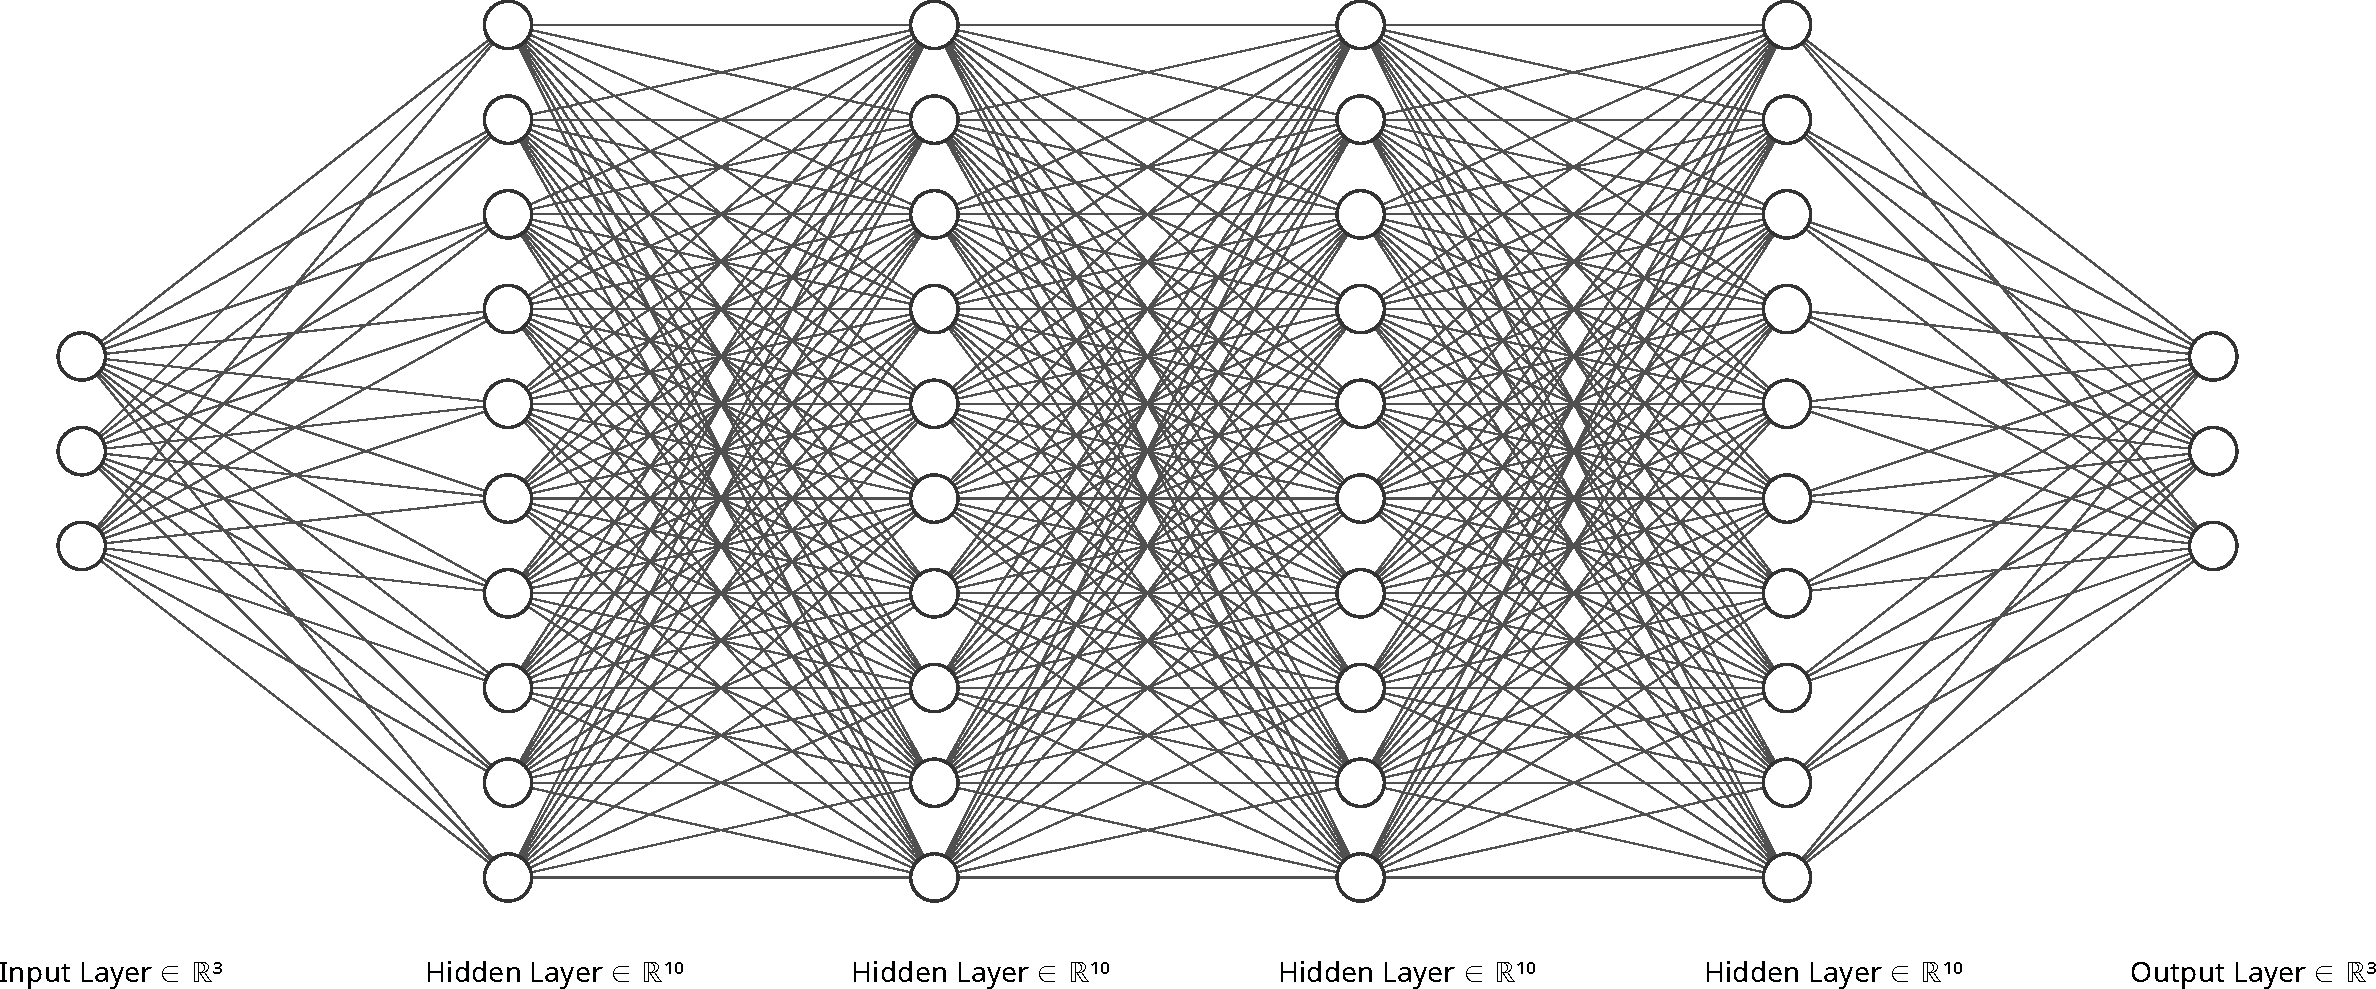
\includegraphics[width=\textwidth]{Figuras/nn.pdf}
    \caption{Artificial Neural Network (ANN) model architecture. Schematic of the Multilayer Perceptron (MLP) used, showing the input layer (3 LF coefficients), ten hidden layers, and the output layer (3 HF coefficients).}
    \label{fig:ann_architecture}
\end{figure}

\begin{figure}[H]
    \centering
    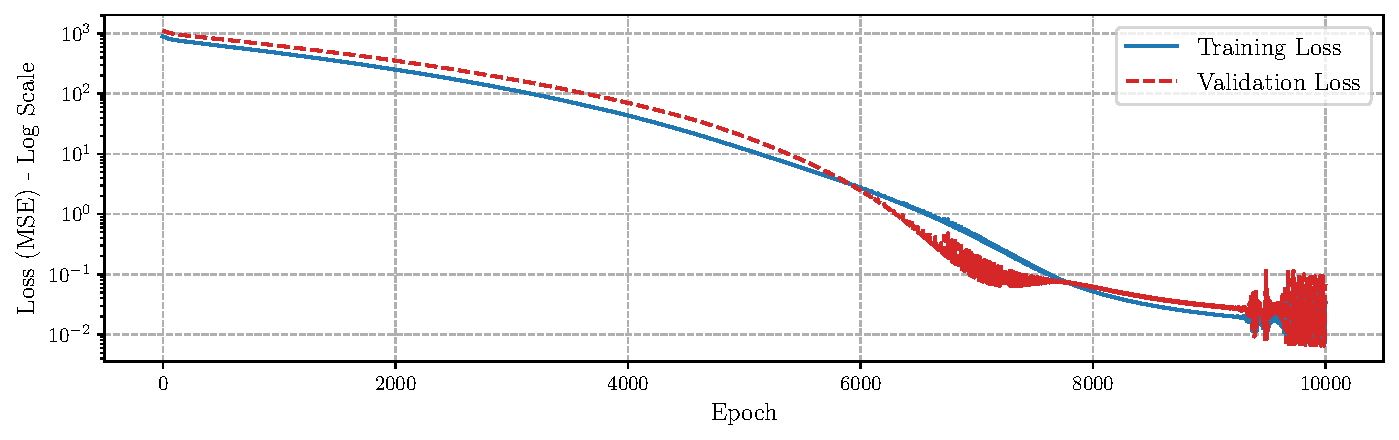
\includegraphics[width=\textwidth]{Figuras/nn_loss.pdf}
    \caption{Learning curve from the ANN training process. Mean Squared Error (MSE) versus training epochs for both the training and validation datasets. The convergence of both curves indicates successful training.}
    \label{fig:ann_loss}
\end{figure}

\subsection{The Kriging Interpolator}

Kriging, also known as Gaussian Process Regression, is a sophisticated statistical interpolation method that has its roots in geostatistics \citep{rasmussen2006, sacks1989}. It frames the interpolation problem from a Bayesian perspective, modeling the unknown function as a realization of a Gaussian process. A prediction at a new point is calculated as a weighted average of the known training data points. Crucially, these weights are not based on simple distance but are determined by a statistical model of spatial correlation (a covariance function or variogram) that is learned from the data itself \citep{jones1998, ng2018}. The Ordinary Kriging predictor for a value at a new point $x_*$ is given by:

\begin{equation}
\hat{f}(x_*) = \hat{\mu} + \mathbf{k}_*^T \mathbf{K}^{-1} (\mathbf{y} - \hat{\mu}\mathbf{1})
\end{equation}

where $\hat{\mu}$ is the estimated mean, $\mathbf{y}$ is the vector of observed training values, $\mathbf{K}$ is the covariance matrix of the training points, and $\mathbf{k}_*$ is the vector of covariances between the training points and the new point. A key advantage of Kriging is that, in addition to providing a prediction (the mean of the posterior distribution), it also provides a measure of the prediction uncertainty (the variance), which can be invaluable for engineering analysis.

Since standard Kriging is a single-output method, a multi-output prediction for the vector $\hat{\mathbf{a}}_h = [\hat{a}_{h,1}, \dots, \hat{a}_{h,d_h}]^T$ is achieved by constructing an independent Kriging model, $f_{\text{Kriging}, i}$, for each of the $d_h$ components of the HF coefficient vector. Each model is trained on the full vector of LF coefficients $\mathbf{a}_l$ to predict its corresponding scalar output component $a_{h,i}$:
\begin{equation}
    \hat{a}_{h,i} = f_{\text{Kriging}, i}(\mathbf{a}_l), \quad \text{for } i=1, \dots, d_h
\end{equation}

The implementation in this study employed ordinary Kriging with an exponential covariance model, assuming no underlying mean bias in the data. The model was trained using the same 145 snapshots from the dataset to learn the correlation structure of the latent space mapping.


\chapter{Analysis of Model Performance and Computational Efficiency}
\label{chap:results_discussion}

\section{Flow Field Reconstruction Accuracy}

The ultimate test of the Reduced Order Models is their ability to accurately reconstruct the full high-fidelity flow field from a new, unseen low-fidelity input. The reconstruction process follows a four-step algorithm:

This reconstruction process follows a four-step algorithm, as detailed below.

\begin{enumerate}
    \item \textbf{Generate a Low-Fidelity Snapshot:}
    For a new set of input parameters, a low-fidelity (LF) simulation is run to obtain the corresponding solution vector, or "snapshot," $\mathbf{x}_l$.

    \item \textbf{Project onto the Low-Fidelity Basis:}
    The new snapshot $\mathbf{x}_l$ is projected onto the pre-computed LF basis, $\mathbf{\Psi}_l$, to obtain its low-dimensional representation (the coefficient vector), $\mathbf{a}_l$.
    \begin{equation}
        \mathbf{a}_l = \mathbf{\Psi}_l^T \mathbf{x}_l
    \end{equation}

    \item \textbf{Map to the High-Fidelity Latent Space:}
    The trained surrogate model, $f_{\text{surrogate}}$, is used to map the low-fidelity coefficients, $\mathbf{a}_l$, to the predicted high-fidelity coefficients, $\hat{\mathbf{a}}_h$.
    \begin{equation}
        \hat{\mathbf{a}}_h = f_{\text{surrogate}}(\mathbf{a}_l)
    \end{equation}

    \item \textbf{Reconstruct the High-Fidelity Flow Field:}
    The full high-fidelity flow field, $\hat{\mathbf{x}}_h$, is reconstructed by combining the predicted HF coefficients, $\hat{\mathbf{a}}_h$, with the pre-computed high-fidelity basis vectors, $\mathbf{\Psi}_h$.
    \begin{equation}
        \hat{\mathbf{x}}_h \approx \mathbf{\Psi}_h \hat{\mathbf{a}}_h
    \end{equation}
\end{enumerate}

% \begin{figure}[H]
%     \centering
%     %\includegraphics[width=0.8\textwidth]{placeholder.png}
%     \caption{Flowchart of the online prediction and reconstruction stage. A new input parameter prompts a fast low-fidelity (LF) simulation. The resulting LF snapshot is projected onto its POD basis to obtain low-dimensional coefficients. The trained surrogate model (ANN or Kriging) maps these to predicted high-fidelity (HF) coefficients, which are then used with the HF POD basis to reconstruct the full HF flow field.}
%     \label{fig:online_reconstruction}
% \end{figure}

\subsection{Neural Network Reconstruction}

The Neural Network-based ROM demonstrated high accuracy. For a representative test case with an inlet total temperature of 927 K, the reconstructed fields were qualitatively very similar to the ground truth full-order model (FOM) results, as shown in Figures \ref{fig:nn_reconstruction_temperature}--\ref{fig:nn_reconstruction_mach}. The maximum absulute relative error obtained on all test dataset occur for the wall heat flux was of only 5.97\%, making most of predicitons almost indistinguishable from the high-fidelity simulation results, as show in figure \ref{fig:nn_reconstruction_heat_flux}, confirming the model's ability to accurately predict the critical quantities of interest.

\begin{figure}[H]
    \centering
    \begin{subfigure}[b]{0.32\textwidth}
        \centering
        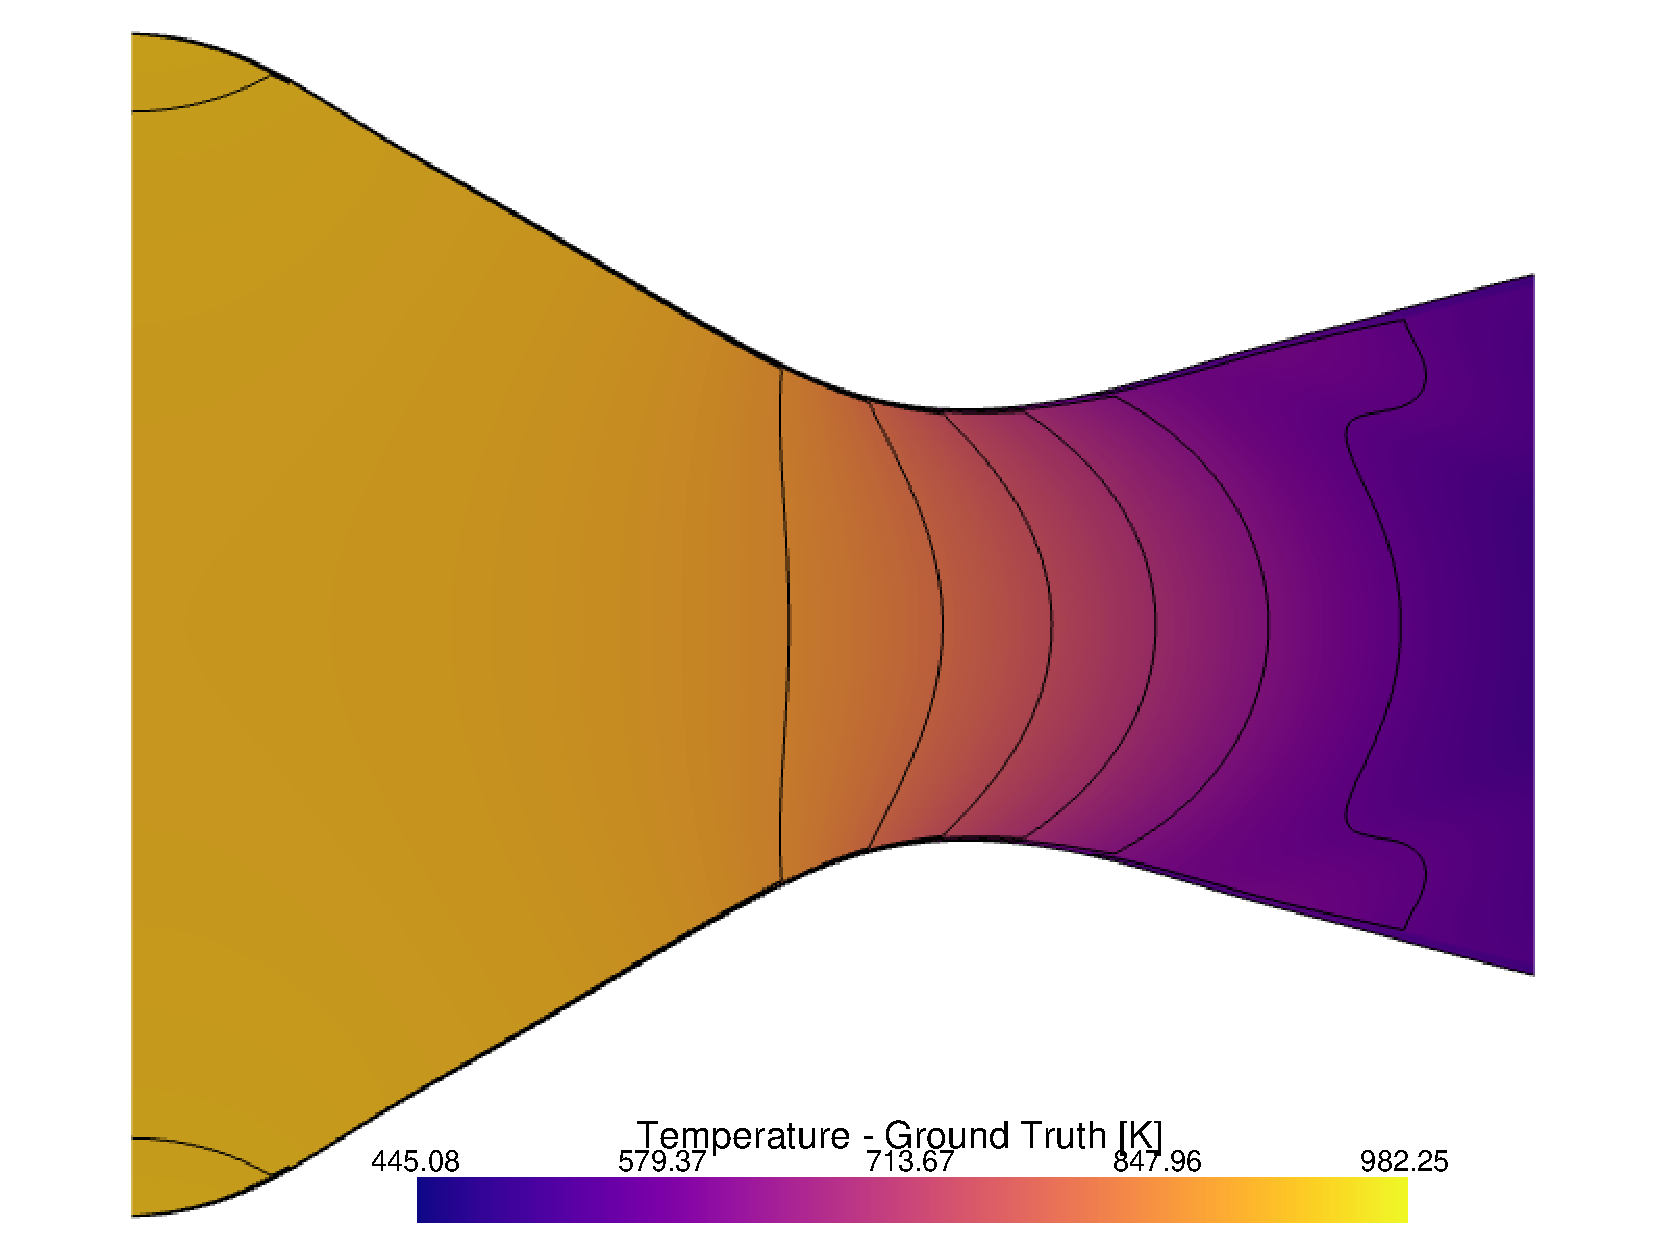
\includegraphics[width=\textwidth]{Figuras/nn_ground_truth_temperature.pdf}
        \caption{FOM}
    \end{subfigure}
    \hfill
    \begin{subfigure}[b]{0.32\textwidth}
        \centering
        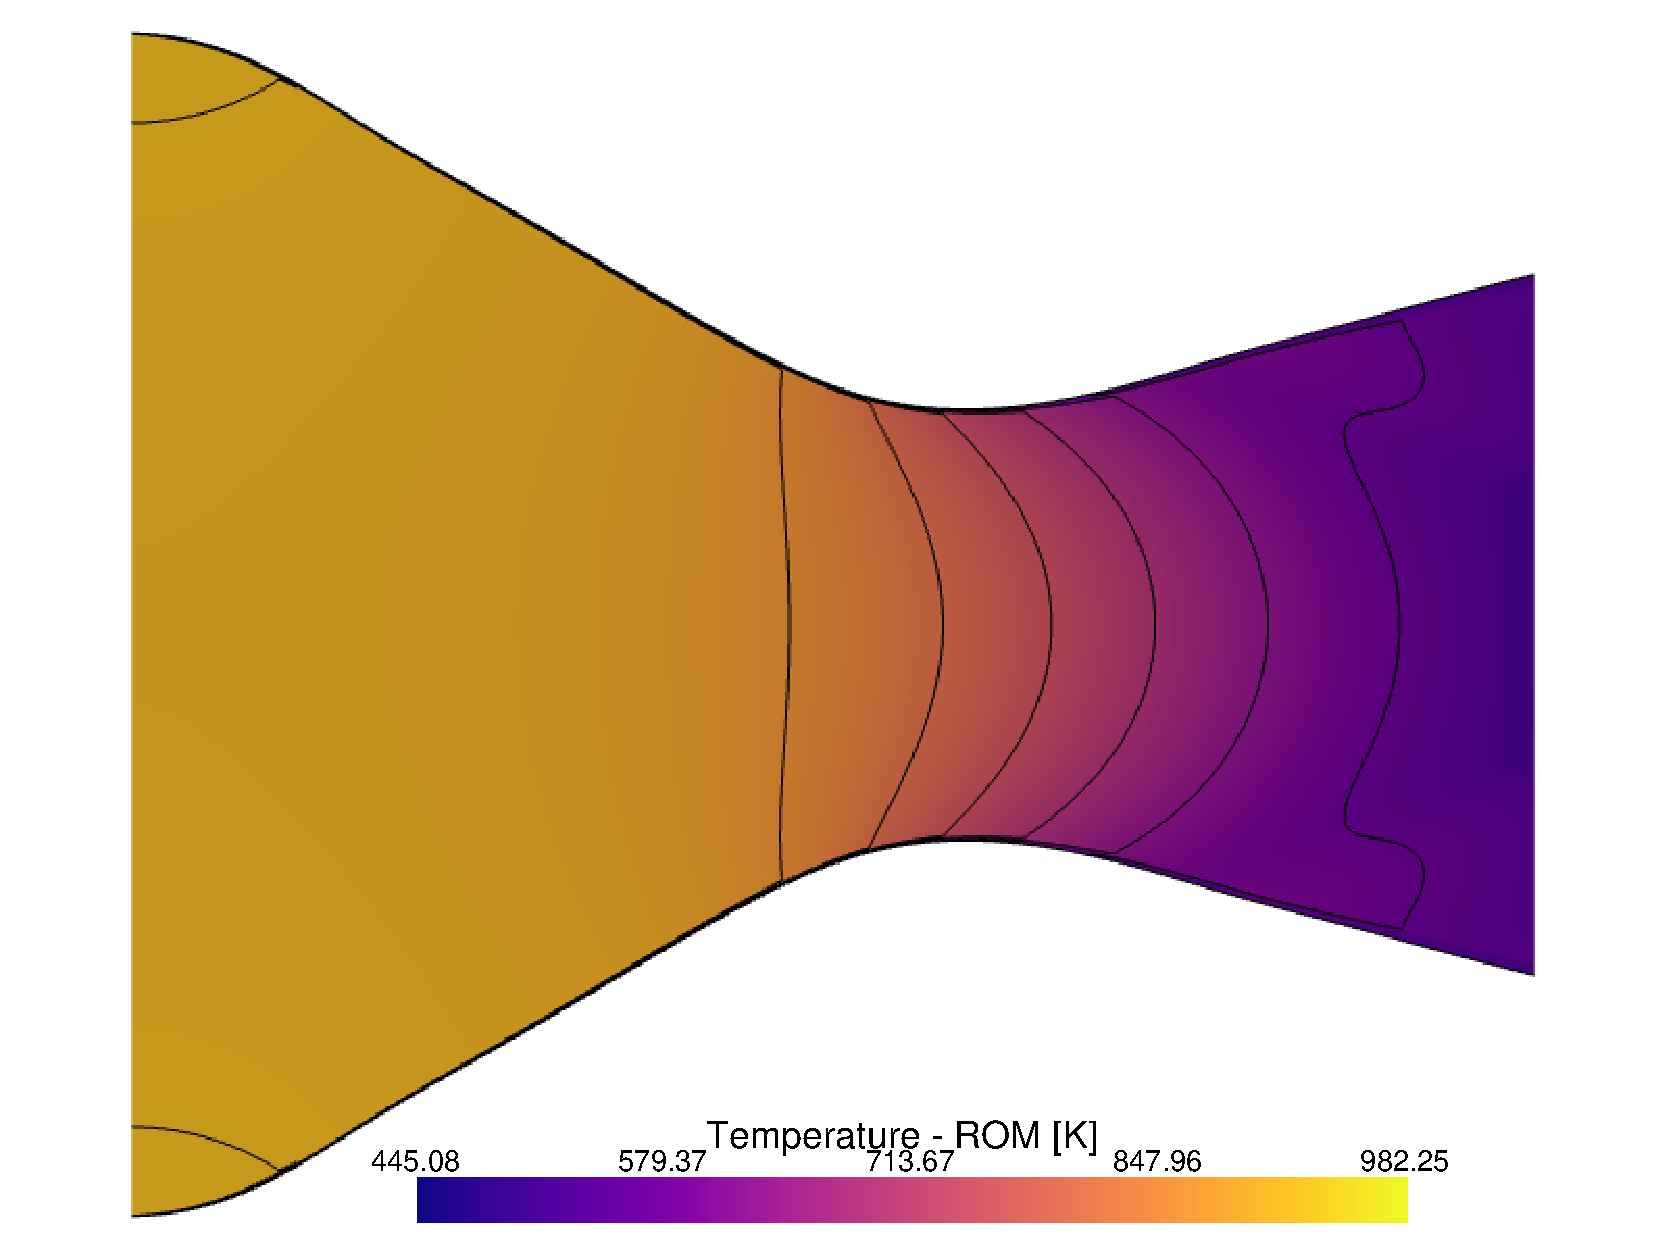
\includegraphics[width=\textwidth]{Figuras/nn_prediction_temperature.pdf}
        \caption{ANN-ROM}
    \end{subfigure}
    \hfill
    \begin{subfigure}[b]{0.32\textwidth}
        \centering
        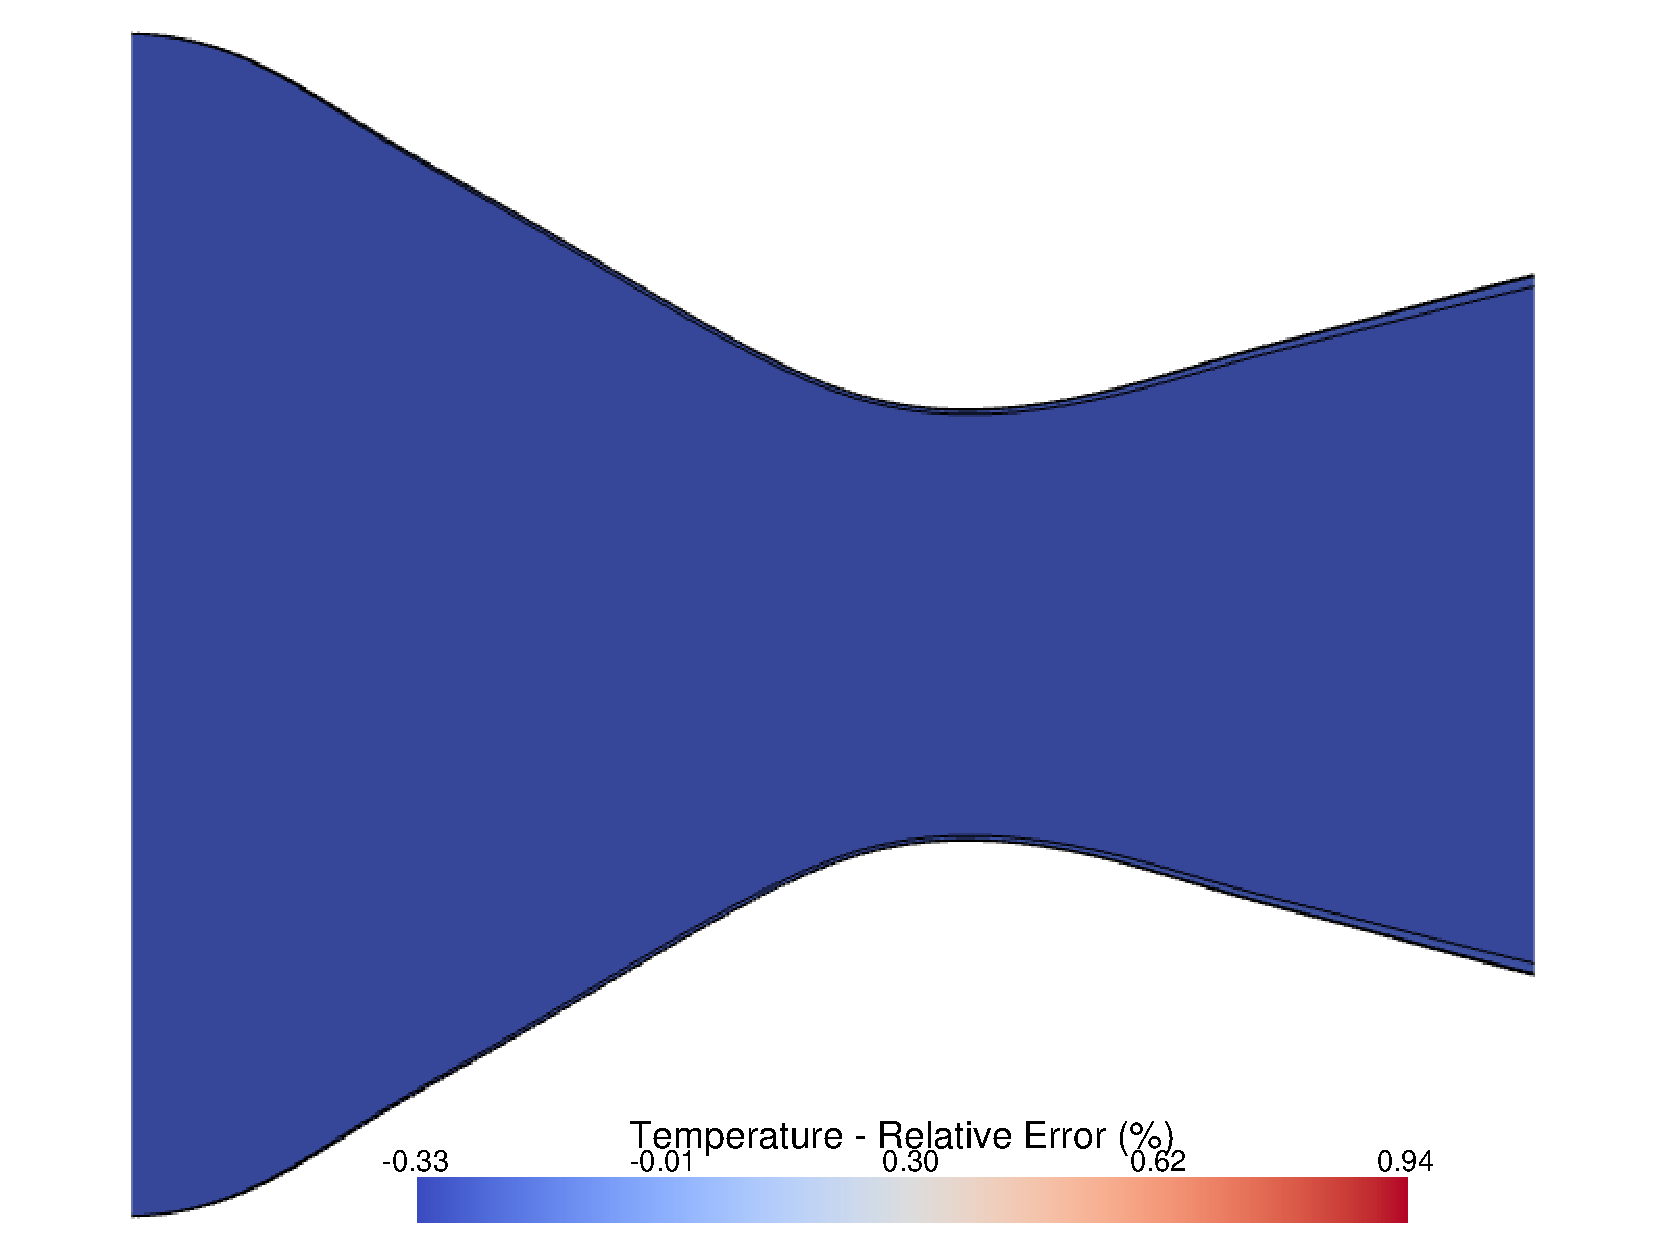
\includegraphics[width=\textwidth]{Figuras/nn_error_temperature.pdf}
        \caption{Error}
    \end{subfigure}
    \caption{Temperature field: (a) ground truth (FOM), (b) ANN-ROM prediction, (c) absolute error.}
    \label{fig:nn_reconstruction_temperature}
\end{figure}

\begin{figure}[H]
    \centering
    \begin{subfigure}[b]{0.32\textwidth}
        \centering
        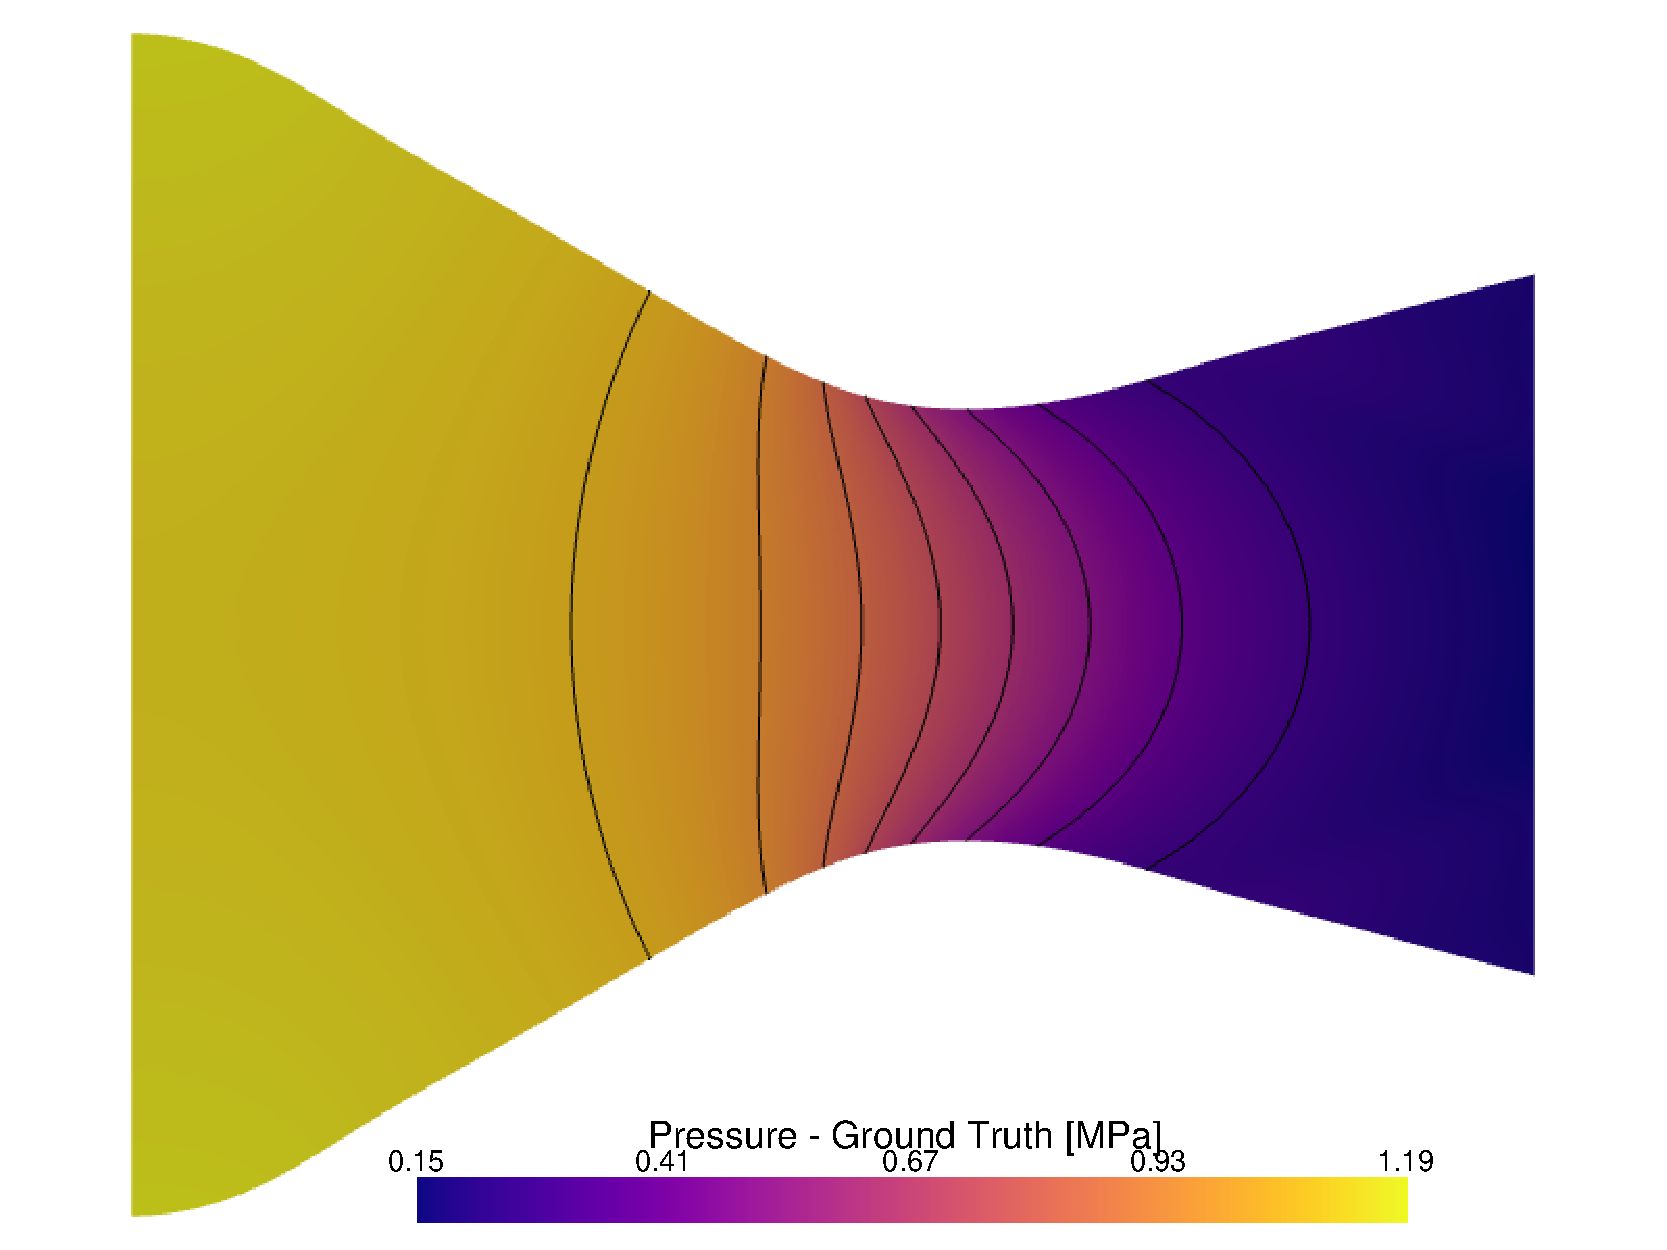
\includegraphics[width=\textwidth]{Figuras/nn_ground_truth_pressure.pdf}
        \caption{FOM}
    \end{subfigure}
    \hfill
    \begin{subfigure}[b]{0.32\textwidth}
        \centering
        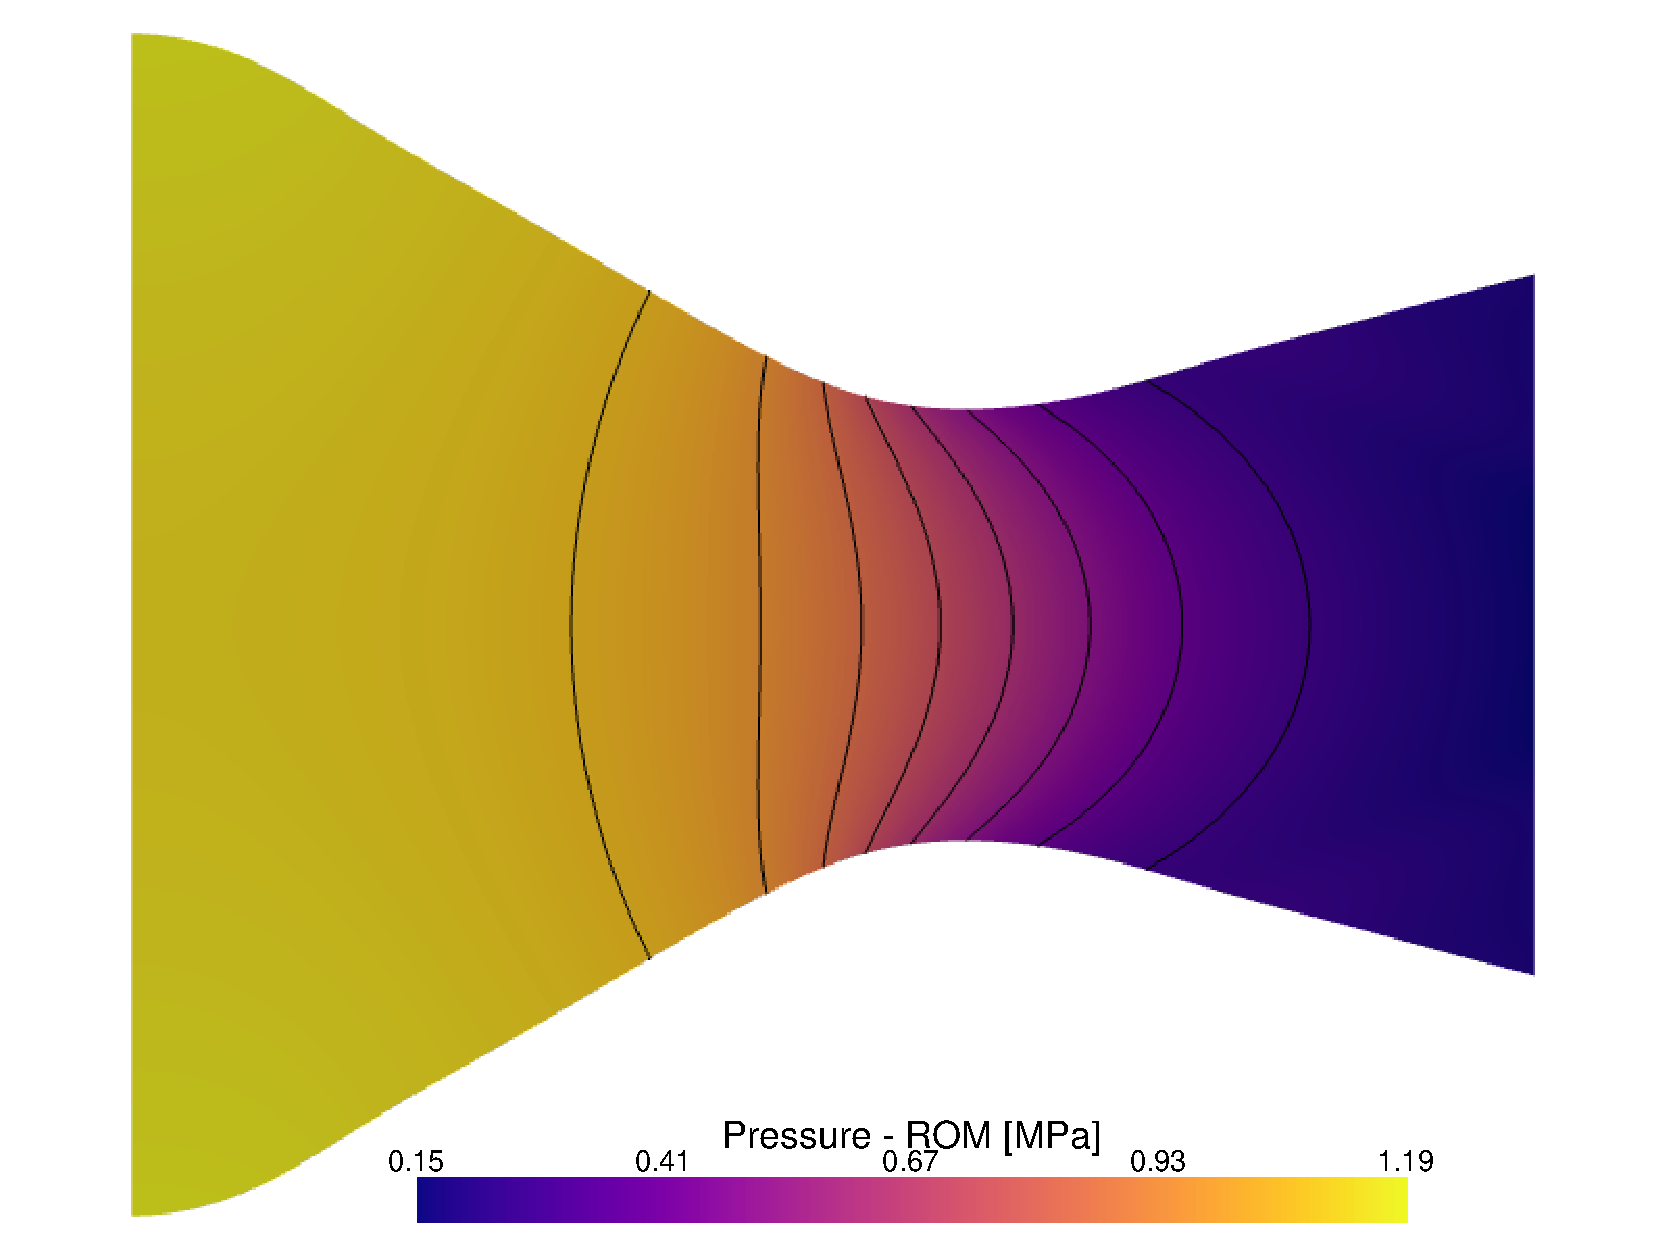
\includegraphics[width=\textwidth]{Figuras/nn_prediction_pressure.pdf}
        \caption{ANN-ROM}
    \end{subfigure}
    \hfill
    \begin{subfigure}[b]{0.32\textwidth}
        \centering
        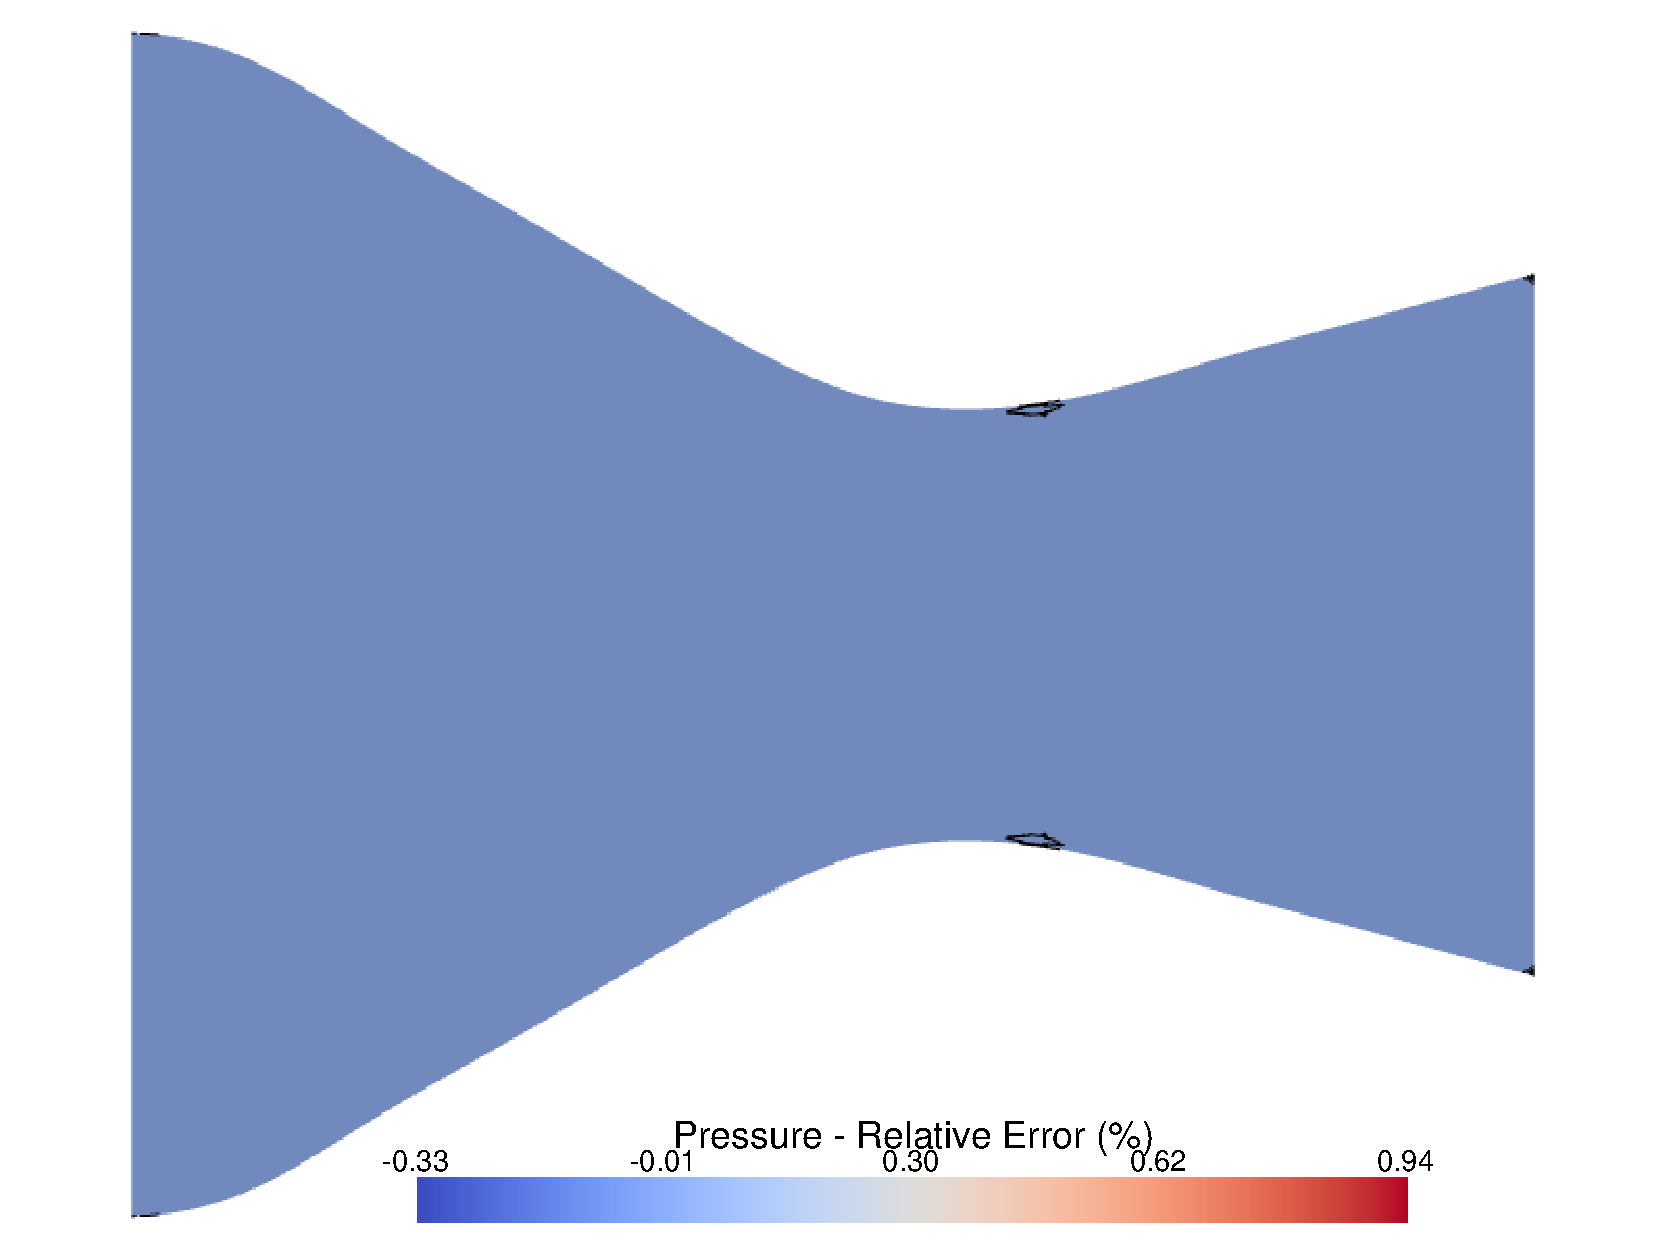
\includegraphics[width=\textwidth]{Figuras/nn_error_pressure.pdf}
        \caption{Error}
    \end{subfigure}
    \caption{Pressure field: (a) ground truth (FOM), (b) ANN-ROM prediction, (c) absolute error.}
    \label{fig:nn_reconstruction_pressure}
\end{figure}

\begin{figure}[H]
    \centering
    \begin{subfigure}[b]{0.32\textwidth}
        \centering
        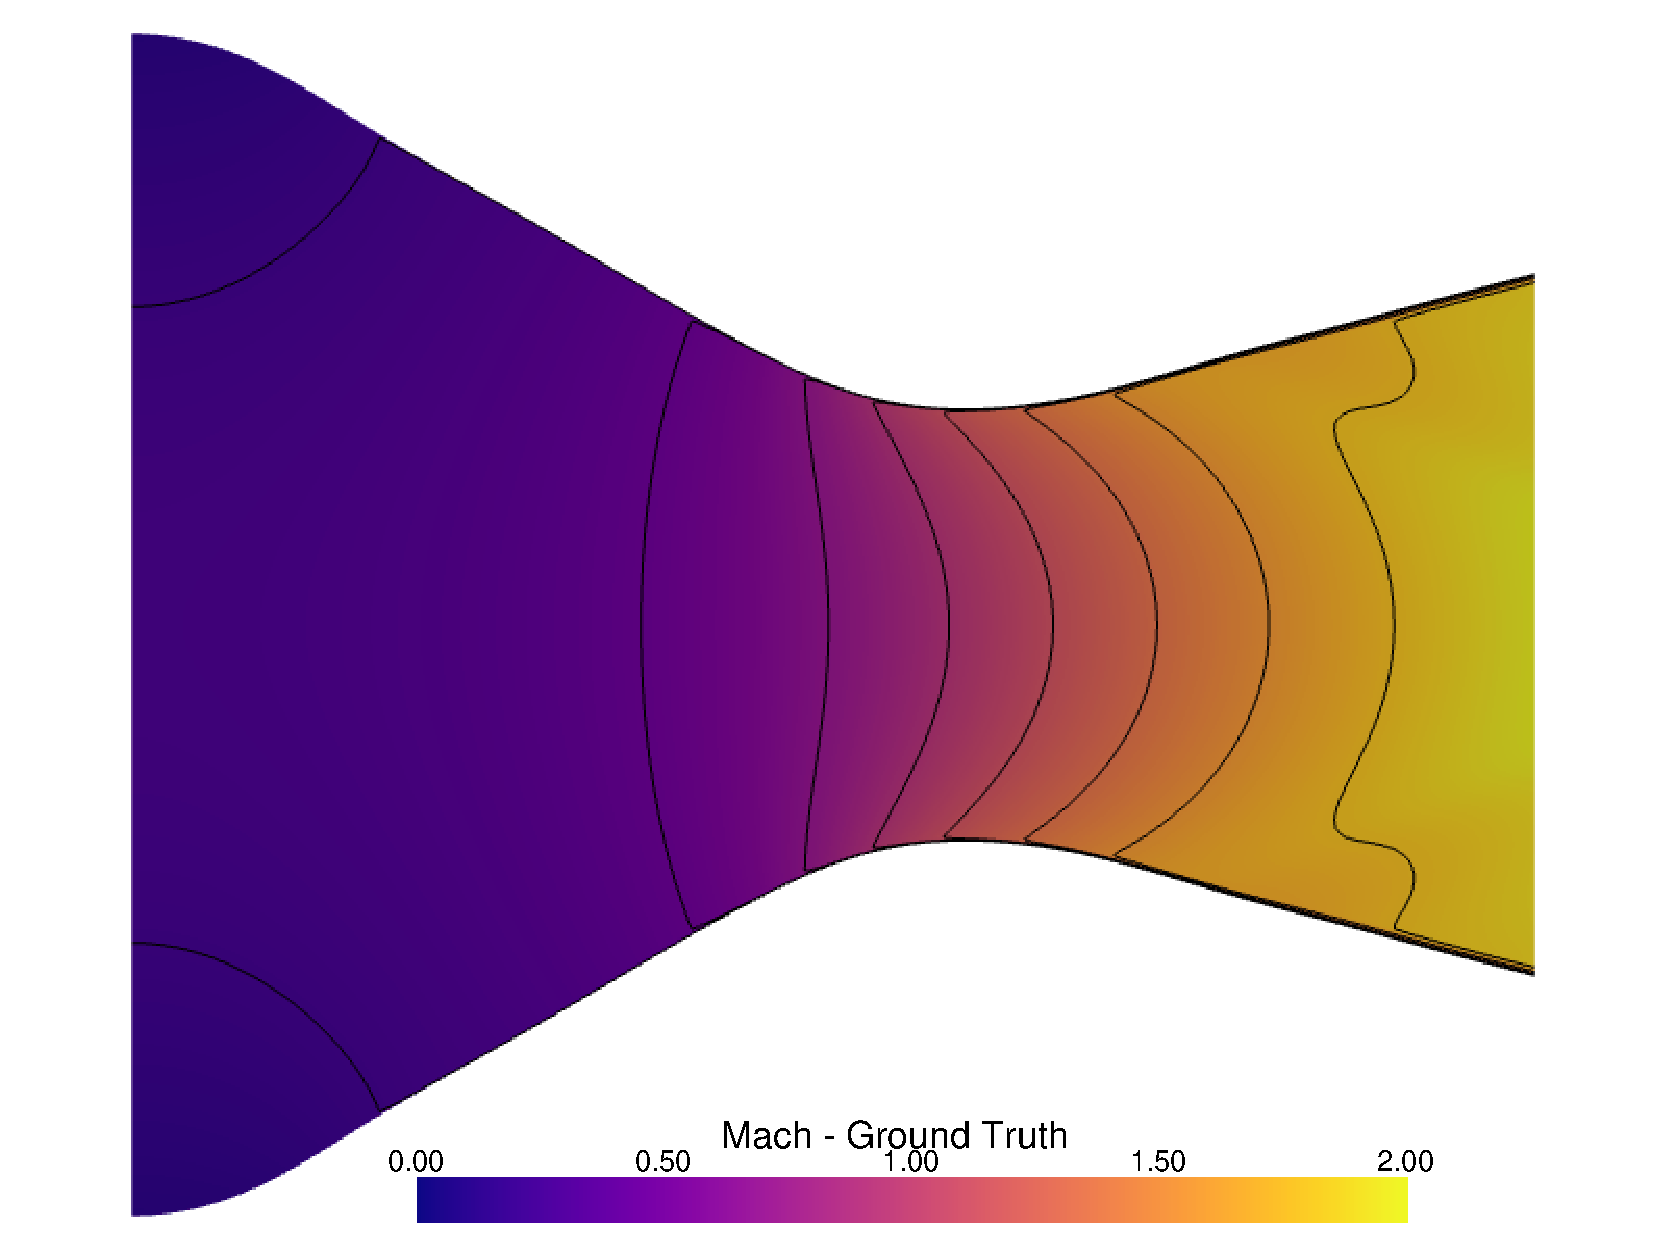
\includegraphics[width=\textwidth]{Figuras/nn_ground_truth_mach.pdf}
        \caption{FOM}
    \end{subfigure}
    \hfill
    \begin{subfigure}[b]{0.32\textwidth}
        \centering
        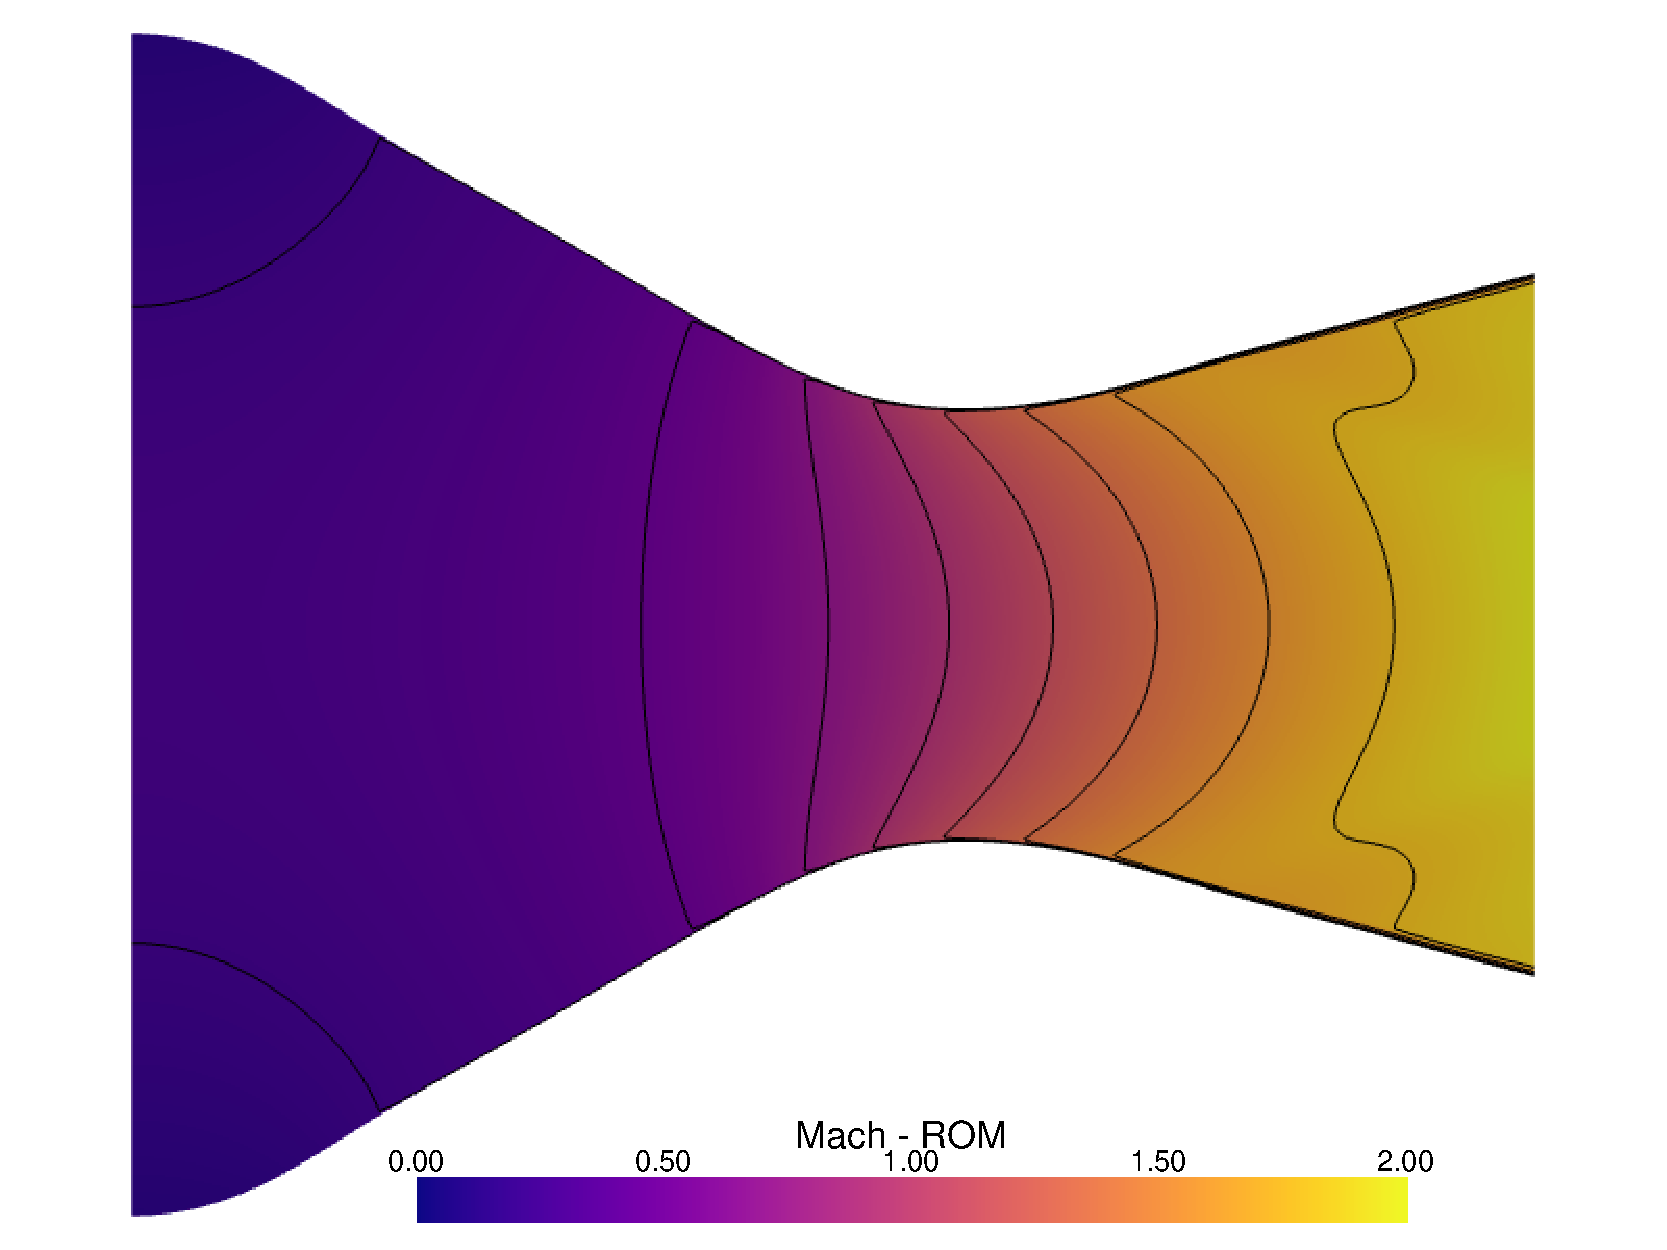
\includegraphics[width=\textwidth]{Figuras/nn_prediction_mach.pdf}
        \caption{ANN-ROM}
    \end{subfigure}
    \hfill
    \begin{subfigure}[b]{0.32\textwidth}
        \centering
        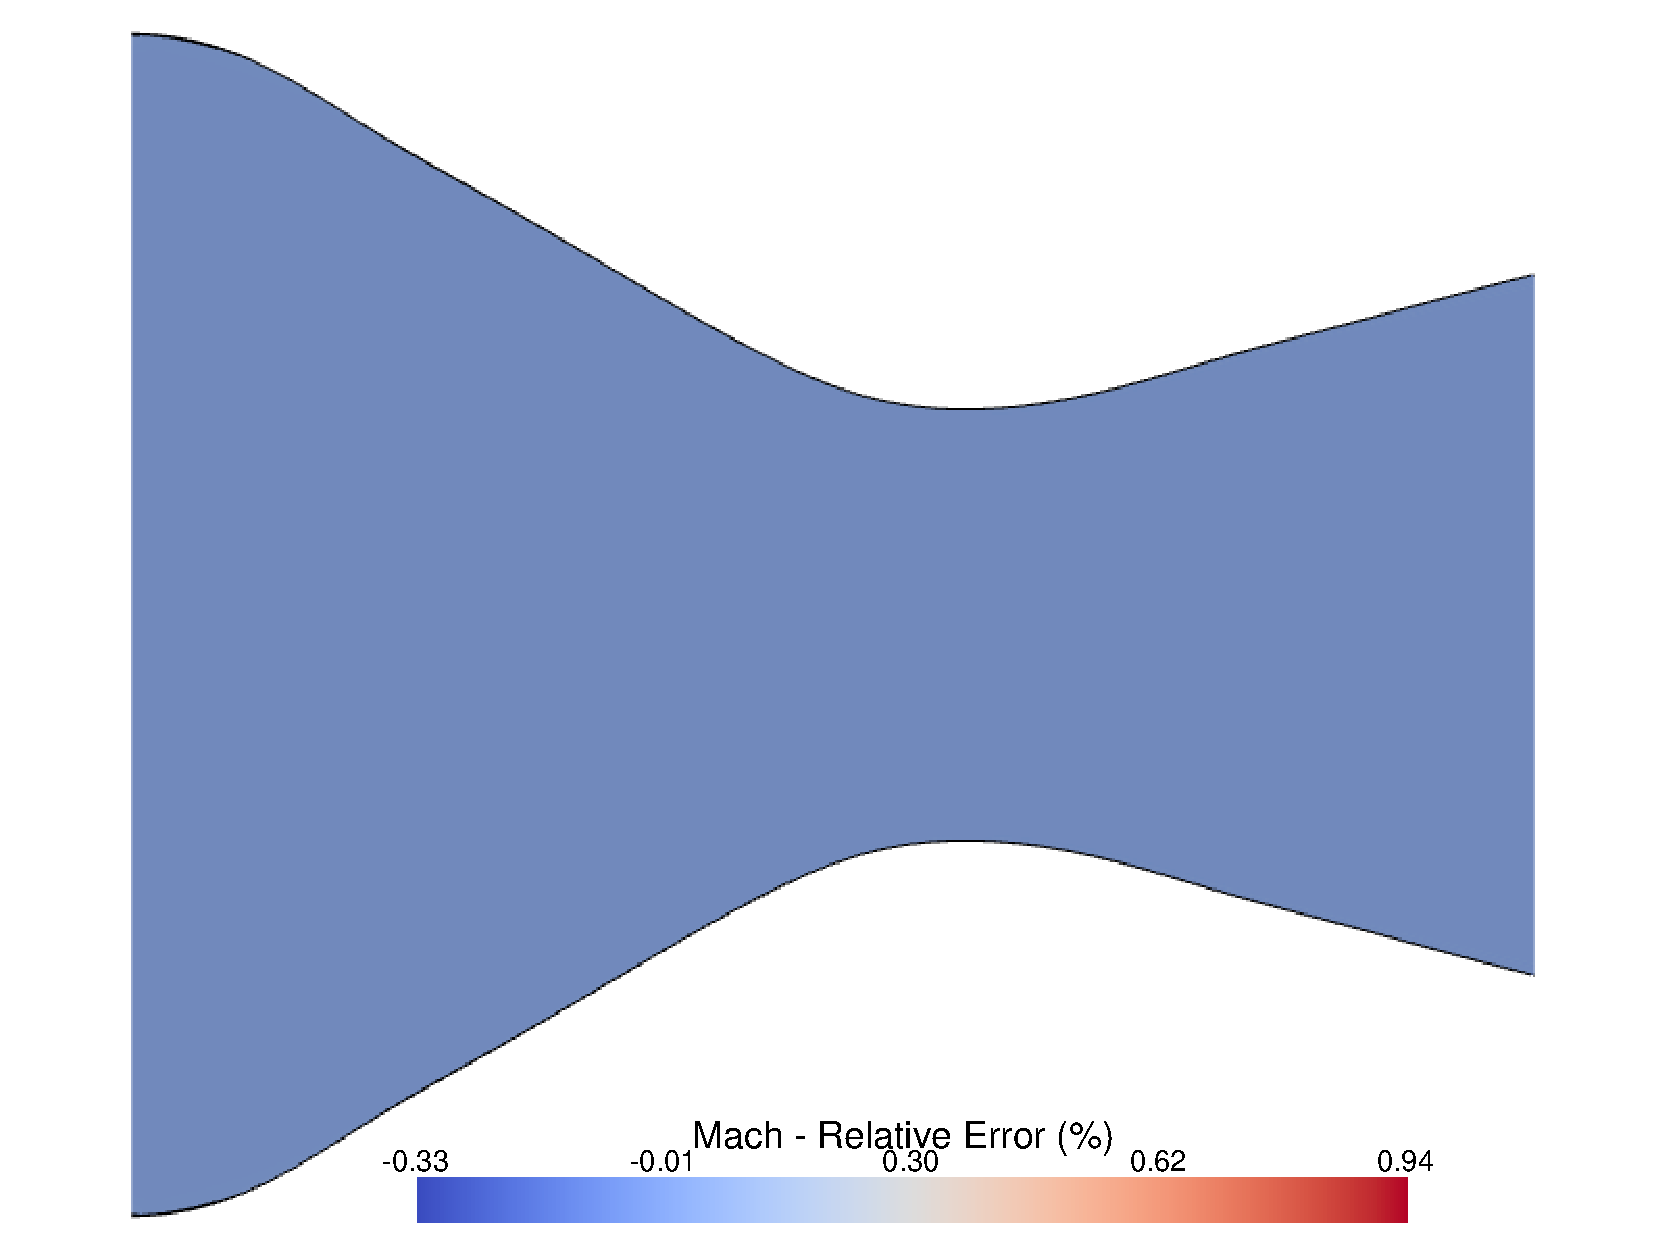
\includegraphics[width=\textwidth]{Figuras/nn_error_mach.pdf}
        \caption{Error}
    \end{subfigure}
    \caption{Mach number field: (a) ground truth (FOM), (b) ANN-ROM prediction, (c) absolute error.}
    \label{fig:nn_reconstruction_mach}
\end{figure}

\begin{figure}[H]
    \centering
    \includegraphics[width=\textwidth]{Figuras/nn_heat_flux.pdf}
    \caption{Comparison of wall heat flux between the FOM and ANN-ROM.}
    \label{fig:nn_reconstruction_heat_flux}
\end{figure}

The Kriging-based ROM achieved even higher accuracy than the neural network approach. For the same representative test case, the reconstructed fields were visually indistinguishable from the ground truth full-order model (FOM) results, as shown in Figures \ref{fig:kriging_reconstruction_temperature}--\ref{fig:kriging_reconstruction_mach}. The maximum absulute relative error obtained on all test dataset also occur for the wall heat flux was of only 5.6\%, slightly lower then ANN conterpart. For most of cases, the predicted wall heat flux distribution was also virtually identical to the high-fidelity simulation, confirming the Kriging model's exceptional predictive capability as show on Figure \ref{fig:kriging_reconstruction_heat_flux}.

\begin{figure}[H]
    \centering
    \begin{subfigure}[b]{0.32\textwidth}
        \centering
        \includegraphics[width=\textwidth]{Figuras/kriging_ground_truth_temperature.pdf}
        \caption{FOM}
    \end{subfigure}
    \hfill
    \begin{subfigure}[b]{0.32\textwidth}
        \centering
        \includegraphics[width=\textwidth]{Figuras/kriging_prediction_temperature.pdf}
        \caption{Kriging-ROM}
    \end{subfigure}
    \hfill
    \begin{subfigure}[b]{0.32\textwidth}
        \centering
        \includegraphics[width=\textwidth]{Figuras/kriging_error_temperature.pdf}
        \caption{Error}
    \end{subfigure}
    \caption{Temperature field: (a) ground truth (FOM), (b) Kriging-ROM prediction, (c) absolute error.}
    \label{fig:kriging_reconstruction_temperature}
\end{figure}

\begin{figure}[H]
    \centering
    \begin{subfigure}[b]{0.32\textwidth}
        \centering
        \includegraphics[width=\textwidth]{Figuras/kriging_ground_truth_pressure.pdf}
        \caption{FOM}
    \end{subfigure}
    \hfill
    \begin{subfigure}[b]{0.32\textwidth}
        \centering
        \includegraphics[width=\textwidth]{Figuras/kriging_prediction_pressure.pdf}
        \caption{Kriging-ROM}
    \end{subfigure}
    \hfill
    \begin{subfigure}[b]{0.32\textwidth}
        \centering
        \includegraphics[width=\textwidth]{Figuras/kriging_error_pressure.pdf}
        \caption{Error}
    \end{subfigure}
    \caption{Pressure field: (a) ground truth (FOM), (b) Kriging-ROM prediction, (c) absolute error.}
    \label{fig:kriging_reconstruction_pressure}
\end{figure}

\begin{figure}[H]
    \centering
    \begin{subfigure}[b]{0.32\textwidth}
        \centering
        \includegraphics[width=\textwidth]{Figuras/kriging_ground_truth_mach.pdf}
        \caption{FOM}
    \end{subfigure}
    \hfill
    \begin{subfigure}[b]{0.32\textwidth}
        \centering
        \includegraphics[width=\textwidth]{Figuras/kriging_prediction_mach.pdf}
        \caption{Kriging-ROM}
    \end{subfigure}
    \hfill
    \begin{subfigure}[b]{0.32\textwidth}
        \centering
        \includegraphics[width=\textwidth]{Figuras/kriging_error_mach.pdf}
        \caption{Error}
    \end{subfigure}
    \caption{Mach number field: (a) ground truth (FOM), (b) Kriging-ROM prediction, (c) absolute error.}
    \label{fig:kriging_reconstruction_mach}
\end{figure}

\begin{figure}[H]
    \centering
    \includegraphics[width=\textwidth]{Figuras/kriging_heat_flux.pdf}
    \caption{Comparison of wall heat flux between the FOM and Kriging-ROM.}
    \label{fig:kriging_reconstruction_heat_flux}
\end{figure}

\section{A Comparative Assessment of Surrogate Modeling Techniques}

A central contribution of this research is the direct, quantitative comparison between the modern machine learning approach (ANN) and the established statistical method (Kriging). The performance of both models, along with the baseline simulations, is synthesized in Table \ref{tab:cost_accuracy_comparison}.

\begin{table}[H]
\centering
\caption{Computational cost and accuracy comparison for Kriging and Neural Network (NN) metamodels. Best results are in \textbf{bold} and worst results in \textit{italics}.}
\label{tab:cost_accuracy_comparison}
\resizebox{\textwidth}{!}{%
\begin{tabular}{l c c c c c c c c c c}
\toprule
& CPU time [s] & \makecell{Speedup \\ w.r.t. \\ High-Fidelity} &
 \multicolumn{2}{c}{Pressure} &
 \multicolumn{2}{c}{Temperature} &
 \multicolumn{2}{c}{Mach} &
 \multicolumn{2}{c}{Heat Flux} \\
& & &
 NRMSE & MaxRelError &
 NRMSE & MaxRelError &
 NRMSE & MaxRelError &
 NRMSE & MaxRelError \\
\midrule
\textbf{High-fidelity model} & 1.53$\times 10^{3}$ & - & - & - & - & - & - & - & - & - \\
\textbf{Low-fidelity model}  & 1.02$\times 10^{0}$ & 1.50$\times 10^{3}$ & - & - & - & - & - & - & - & - \\
\textbf{NN training} & 3.17$\times 10^{2}$ & - &
 \textit{2.08$\times 10^{-6}$} & \textit{2.48$\times 10^{-2}$} &
 \textit{2.12$\times 10^{-3}$} & \textit{5.70$\times 10^{-1}$} &
 \textit{5.77$\times 10^{-5}$} & \textit{1.06$\times 10^{0}$} &
 \textit{1.28$\times 10^{-3}$} & \textit{5.97$\times 10^{0}$} \\
\textbf{Kriging training} & \textbf{5.70$\times 10^{0}$} & - &
 \textbf{1.89$\times 10^{-6}$} & \textbf{2.43$\times 10^{-2}$} &
 \textbf{5.50$\times 10^{-5}$} & \textbf{3.95$\times 10^{-1}$} &
 \textbf{4.24$\times 10^{-5}$} & \textbf{9.96$\times 10^{-1}$} &
 \textbf{3.07$\times 10^{-4}$} & \textbf{5.60$\times 10^{0}$} \\
\textbf{Single NN evaluation} & 2.30$\times 10^{-1}$ & 6.66$\times 10^{3}$ & - & - & - & - & - & - & - & - \\
\textbf{Single Kriging evaluation} & \textbf{4.00$\times 10^{-2}$} & \textbf{3.83$\times 10^{4}$} & - & - & - & - & - & - & - & - \\
\bottomrule
\end{tabular}%
}
\end{table}




The results clearly show that while both ROMs provide massive speedups, the Kriging model is superior in every metric: it is faster to train, faster to evaluate, and slightly more accurate. This counter-intuitive result, where a "classic" statistical method outperforms a more "modern" neural network, warrants deeper analysis. The reason for Kriging's superior performance likely lies in the specific nature of this engineering problem: a relatively small training dataset (145 points) is used to learn a smooth, low-dimensional mapping (10 input variables to 10 output variables). Artificial Neural Networks are highly flexible models with a large number of free parameters (weights and biases). While this flexibility is a great strength for complex, high-dimensional problems with vast amounts of data, it can be a weakness with smaller datasets, where the network may struggle to generalize perfectly. Kriging, in contrast, is a method specifically designed for interpolation from sparse data \citep{jones1998, ng2018}. Its underlying statistical assumptions—that the function is a realization of a Gaussian process with a certain spatial correlation—provide a strong "inductive bias". This bias constrains the model, guiding it to find the best linear unbiased predictor based on the correlations observed in the limited training data \citep{rasmussen2006, sacks1989}. For this particular problem, Kriging's statistically-grounded approach proved to be a more efficient and robust strategy for interpolation than the more flexible but less constrained neural network. This finding serves as an important reminder for the engineering community: the application of complex deep learning models is not always the optimal path, and mature statistical techniques should be carefully considered, as they may be more appropriate and effective for the problem at hand.

\section{Evaluation of Computational Gains and Engineering Impact}

The practical implications of this research are profound. The Kriging-based ROM achieves a speedup of over 38,000 times compared to the high-fidelity simulation, reducing a computation that takes over 25 minutes to just 0.04 seconds, with negligible loss in accuracy \citep{moreira2023}. This dramatic acceleration transforms the landscape of what is possible in nozzle design and analysis.

Previously infeasible studies are now brought within reach. For instance, a comprehensive multi-objective design optimization, which might require tens of thousands of function evaluations to explore trade-offs between performance and structural integrity, can now be performed in hours instead of years \citep{deb2002, toffol2018}. Full-scale uncertainty quantification, propagating uncertainties in manufacturing tolerances or operational conditions through the model to predict the reliability of the design, becomes a tractable problem \citep{ng2018, lemaitre2010}. Furthermore, the near-instantaneous prediction speed opens the door to applications in inverse design (determining the nozzle shape required to produce a desired flow field) and even real-time control systems for advanced propulsion concepts \citep{moreira2023, hesthaven2016}.

\chapter{Synthesis, Conclusions, and Future Directions}
\label{chap:conclusions_future_work}

\section{Synthesis of Findings}

This dissertation has successfully detailed the development and validation of a multi-fidelity, data-driven framework capable of accelerating the aerothermodynamic analysis of convergent-divergent nozzles by orders of magnitude. The key achievements of this work can be synthesized as follows:
\begin{itemize}
    \item A robust multi-fidelity simulation workflow was established, coupling a high-fidelity 2D RANS-CHT solver (SU2) with a computationally inexpensive quasi-1D Euler solver. Both models were rigorously verified and validated.
    \item Proper Orthogonal Decomposition was shown to be exceptionally effective at dimensionality reduction, compressing the high-dimensional state of the flow field into a compact latent space of only 10 variables with minimal information loss.
    \item Two distinct machine learning-based surrogate models—an Artificial Neural Network and a Kriging interpolator—were successfully implemented and trained to map the low-fidelity latent space to the high-fidelity latent space.
    \item Quantitative analysis demonstrated that the resulting Reduced Order Models can reconstruct the high-fidelity flow field and critical wall heat transfer quantities with high accuracy, achieving a computational speedup of up to 38,000 times over the full-order model.
\end{itemize}

\section{Concluding Remarks}

The central conclusion of this work is twofold. First, it confirms that data-driven, non-intrusive Reduced Order Models provide a powerful and effective strategy for bridging the fidelity gap in the computational analysis of complex engineering systems like rocket nozzles. They successfully leverage the speed of simple models and the accuracy of complex ones, breaking the traditional compromise between computational cost and predictive fidelity. Second, and perhaps more significantly, this study demonstrates that for engineering problems characterized by smooth, low-dimensional mappings and limited data availability, established statistical methods like Kriging can outperform more complex, modern deep learning architectures in terms of accuracy, training cost, and evaluation speed. This highlights the critical importance of selecting a modeling technique that is appropriate for the specific structure and scale of the problem at hand.

\section{Future Directions and Broader Impact}

While this study has established a successful framework, several promising avenues for future research exist that could extend its capabilities and impact.

\begin{itemize}
    \item \textbf{Geometric Variations:} The current model is parameterized only by an inlet boundary condition. A significant extension would be to incorporate variations in the nozzle geometry itself, such as the contour shape or throat radius. This would require a more sophisticated parameterization of the geometry (e.g., using B-splines or Class Shape Function Transformations) and a substantially larger training dataset to cover the expanded design space \citep{bekemeyer2025, samareh2001}.
    \item \textbf{Extension to 3D:} Applying this methodology to full three-dimensional nozzle simulations is the next logical step toward industrial relevance. This presents significant challenges, as the computational cost of the HF model and the sheer size of the data snapshots increase by orders of magnitude, demanding more advanced data handling and potentially more sophisticated ROM techniques \citep{carlberg2018}.
    \item \textbf{Advanced ROM Techniques:} Future work could explore more advanced data-driven methods. For non-linear dimensionality reduction, deep autoencoders could be investigated as an alternative to the linear basis of POD \citep{erichson2020, kutz2017}. For unsteady flows, where transient behavior is important, methods like Dynamic Mode Decomposition (DMD) could be employed to capture the temporal dynamics of the system \citep{hesthaven2016, rowley2017}.
    \item \textbf{Integration into Optimization Loops:} The validated Kriging-based ROM is an ideal candidate for integration into a formal design optimization framework. It could be coupled with a multi-objective genetic algorithm, such as NSGA-II, to perform rapid optimization of the nozzle shape or its cooling channel design to maximize performance while respecting thermal constraints \citep{deb2002}.
    \item \textbf{Uncertainty Quantification:} The Kriging model's inherent ability to provide a prediction variance should be fully exploited. This would enable a comprehensive Uncertainty Quantification (UQ) analysis, allowing designers to understand how uncertainties in input parameters (e.g., material properties, operating conditions) propagate to uncertainties in key performance metrics, leading to more robust designs \citep{yu2019, ng2018, lemaitre2010}.
\end{itemize}

The impact of this research contributes to the ongoing shift in engineering design towards a "digital twin" paradigm. By creating fast and accurate virtual representations of physical assets, these data-driven models enable continuous monitoring, real-time optimization, and predictive maintenance, paving the way for the next generation of intelligent and efficient aerospace systems \citep{glaessgen2012digital, rasheed2020}.



\newpage
\bibliographystyle{Bibliografia/abnt2023}
\bibliography{Bibliografia/library}

\end{document}
% ----------------------------------------------------------
%% End of file `Relatorio_TCC_Mestrado_Base_x_y_autor.tex'.
